\documentclass[11pt,a4paper]{article}

\usepackage[margin=1in]{geometry}
\usepackage[T1]{fontenc}
\usepackage{lmodern}
\usepackage{amsmath,amssymb,amsthm}
\usepackage{mathtools}
\usepackage[protrusion=true,expansion=false]{microtype}
\usepackage{hyperref}
\usepackage{booktabs}
\usepackage{tabularx}
\usepackage{graphicx}
\usepackage{xcolor}
\usepackage{enumitem}
\usepackage{caption}
\usepackage{tikz}
\usepackage{pgfplots}
\pgfplotsset{compat=1.18}
\usetikzlibrary{positioning,arrows.meta,fit,backgrounds,calc,shapes.geometric,decorations.pathreplacing,patterns}
\usepgfplotslibrary{groupplots}
% Categorical palette (fixed order) and neutrals for every figure.
\definecolor{cA}{HTML}{2A78D6}  % blue: representation / arithmetic
\definecolor{cB}{HTML}{EB6834}  % orange: instruction (hardware feature)
\definecolor{cC}{HTML}{1BAF7A}  % aqua: memory / layout
\definecolor{cD}{HTML}{EDA100}  % yellow: launch geometry
\definecolor{cE}{HTML}{6250D6}  % violet
\definecolor{inkS}{HTML}{52514E}
\definecolor{gridc}{HTML}{D9D8D3}
\definecolor{boxfill}{HTML}{F4F3EF}
\pgfplotsset{every axis/.append style={axis line style={inkS},tick style={inkS},
  major grid style={gridc},label style={font=\small},tick label style={font=\footnotesize},
  legend style={font=\footnotesize,draw=none,fill=none}}}
\usepackage[numbers,sort&compress]{natbib}
\usepackage{url}
\usepackage{xurl}

\hypersetup{
  pdftitle={Accelerating Pollard Rho with GPU Field Arithmetic on NVIDIA Blackwell},
  pdfauthor={Anonymous},
  colorlinks=true,
  linkcolor=blue!50!black,
  citecolor=blue!50!black,
  urlcolor=blue!50!black,
}

\newtheorem{theorem}{Theorem}[section]
\newtheorem{lemma}[theorem]{Lemma}
\newtheorem{proposition}[theorem]{Proposition}
\theoremstyle{definition}
\newtheorem{definition}[theorem]{Definition}
\newtheorem{remark}[theorem]{Remark}

\newcommand{\FF}{\mathbb{F}}
\newcommand{\ZZ}{\mathbb{Z}}
\newcommand{\QQ}{\mathbb{Q}}
\newcommand{\HW}{\operatorname{HW}}
\renewcommand{\gcd}{\operatorname{gcd}}
\newcommand{\Bs}{\,\text{billion iterations/s}}
\newcommand{\thisrepo}{\texttt{crypto}}
\newcommand{\sibling}{\texttt{cryptanalysis}}
% Evidence records (Appendix B). \evcite{\evref{key}, §x; \evref{key2}}
% prints [E3, §x; E7]; each record is numbered in order of first citation.
\newcounter{evrec}
\newcommand{\evlabel}[2]{\refstepcounter{evrec}\label{ev:#1}E\theevrec}
\newcommand{\evref}[1]{\hyperref[ev:#1]{E\ref*{ev:#1}}}
\newcommand{\evcite}[1]{[#1]}

\title{Accelerating Pollard Rho with GPU Field Arithmetic\\
       on NVIDIA Blackwell}
% Anonymized for double-blind submission.  Author block restored
% for camera-ready / preprint release; see README.md.
\author{Anonymous}
\date{}

\begin{document}
\maketitle
\emergencystretch=2em

\begin{abstract}
\input{abstract.txt}
\end{abstract}

\tableofcontents
\clearpage

\section{Introduction}
\label{sec:intro}

In 1997 Certicom published a list of elliptic-curve discrete
logarithm challenges~\cite{certicom1997}. Three of them, ECC2K-95,
ECC2K-108 and ECC2K-130, use the Koblitz curve $y^2+xy=x^3+1$ over
$\FF_{2^{97}}$, $\FF_{2^{109}}$ and $\FF_{2^{131}}$ and ask for the $k$
with $Q=[k]P$. Harley's group solved ECC2K-95 in 1998~\cite{harley1998}
and ECC2K-108 in 2000. ECC2K-130 is still open. In 2009 a consortium of
twenty authors published the arithmetic, the iteration function and
per-platform throughput for an attack on
it~\cite{bailey2009,bailey2009sharcs,bos2010cell,fan2010fpga}, and
estimated the work at $2^{60.9}$ iterations. That attack was never
completed.

This paper is about what Pollard rho costs on the current generation
of NVIDIA hardware, and ECC2K-130 is the yardstick. In 2009 the
fastest GPU in the consortium's plan had no carry-less multiplier and
a binary-field product had to be built bit by bit from AND and XOR
(Section~\ref{sec:history}). Today CUDA~13.3 exposes a carry-less
multiply-add, \texttt{clmad}, in PTX; on this walk a Blackwell SM retires
integer logic at about twice an Ada SM's per-clock rate; and three-input logic, funnel
shifts and byte permutes all issue at full rate. We rebuilt the
ECC2K-130 attack from scratch around that hardware and measured, step
by step, how far each change moves the rate. On one RTX~PRO~6000
Blackwell the campaign's walk runs at $14.64$ billion iterations per
second in its audited build and $15.88$ in the best later build, about
$230$ times the best published GTX~295 kernel of
2010~\cite{bernstein2010gpu}, so the whole $2^{60.9}$ budget is now
about five GPU-years (Section~\ref{sec:history-compare}).

We also wanted to know which of those gains belong to binary fields
and which belong to rho on GPUs in general. So we carried the same
optimisations to Pollard rho on NIST P-256 and P-384, on the same card.
Most of the levers transferred; their relative sizes did not.

We tried to hold the work to the standard the first attempt's reports
set, and in places to a stricter one: every rate is paired against an
adjacent control on the same machine, every target was written down
before we tuned toward it, and every claim cites the evidence record
that backs it. None of this improves on the
generic-group bound, and we do not pretend otherwise. What we report is
the cost of one step on GPUs, CPUs and an FPGA; the number of steps,
measured on small curves of the same family and extrapolated; and a
campaign that has walked $2^{56.7}$ of the $2^{60.9}$ iterations, most of
it before its cloud fleet was taken away.

All rates in this paper are in billions of iterations per second on
one device unless a row says otherwise. An iteration is one complete
step of one walk, including its share of the batched inversion, the
distinguished-point test and the restart path.

\paragraph{Contributions.}
\begin{itemize}[leftmargin=1.2em,itemsep=0.3em]
\item A side-by-side account of ECC2K-130 rates on 2009--2010 hardware
  and on current GPUs, in one unit (Section~\ref{sec:history}).
\item Background on the instructions this arithmetic relies on, from
  Fermi's \texttt{PRMT} to the PTX~9.3 \texttt{clmad}, and on x86, Arm and
  RISC-V from \texttt{PCLMULQDQ} to AVX-512, SVE2 and Zvbc
  (Section~\ref{sec:isa}).
\item A measured description of what current NVIDIA hardware changes
  for rho: the PTX~9.3 \texttt{clmad} instruction, its rate on three
  dies (from $1.69$ lanes per SM-clock on the RTX~PRO~6000 to $29.9$ on
  the H100), and why the same source change can win on one Blackwell
  part and lose on another (Section~\ref{sec:blackwell}).
\item Diagrams of the kernel itself (thread layout, the step's data
  flow, the carry-less product, the memory layout) and a breakdown of
  where the speedup came from by kind of change. None of it changed the
  algorithm (Section~\ref{sec:what-changed}).
\item A GPU ledger of sixteen paired optimisation steps, taking one
  RTX~PRO~6000 from $0.85$ to $14.64$ billion iterations per second for
  the campaign build, with later $\sigma$-walk builds at $15.44$ and
  $15.88$, a roofline, a floor derived from the carry-less unit before
  tuning that rules out $28$ on one card, and every candidate we built
  and rejected (Section~\ref{sec:gpu}).
\item A clear separation of the $\sigma$-walk from the table walk. The
  table walk's $20.08$ was measured under a cycle rule later found to
  exit cycles inconsistently; the exact rule runs at $8.24$ today, so
  the $\sigma$-walk is the fastest correct walk we have
  (Section~\ref{sec:sigma-vs-table}).
\item Measurements on twelve GPUs from Turing to Blackwell, per card,
  per SM and per dollar (Section~\ref{sec:survey}).
\item The same ladder applied to Pollard rho on NIST P-256 and P-384 on
  the RTX~PRO~6000: $1.52\times$ and $2.61\times$ over the first working
  build, to $1.632$ and $0.548$ billion iterations per second
  (Section~\ref{sec:nist}).
\item Supporting work: a code generator that builds every field routine
  from one checked model of $\FF_{2^{131}}$
  (Sections~\ref{sec:curve} and \ref{sec:arith}); walk constants
  measured rather than assumed, $2^{60.91}$--$2^{60.92}$ iterations for
  the campaign's walk (Section~\ref{sec:walk}); bitsliced CPU clients
  (Section~\ref{sec:cpu}); an inventory of the repositories' other GPU
  kernels (Section~\ref{sec:othergpu}); an FPGA engine at $8.25$ billion
  iterations per second on one AWS F2 (Section~\ref{sec:fpga}); and the
  campaign at $486$~M points and $2^{56.68}$ iterations
  (Section~\ref{sec:campaign}).
\item CPU measurements by instruction set: AVX2, AVX-512's ternary
  logic, and NEON with \texttt{BSL} and \texttt{EOR3}
  (Section~\ref{sec:cpu}).
\item Upper bounds per platform: about $24$--$26$ billion iterations per
  second for any one-addition walk on one RTX~PRO~6000, a $1.55\times$
  logic cut for $30$ on a B200, $9.3$ for the F2 FPGA, and $4.6$--$12.2$ for
  the NIST walk, with what each would mean for the cost of a solve
  (Section~\ref{sec:bounds}).
\item The time to a solve on every measured device and fleet size,
  including rho's spread and the detection delay of the
  distinguished-point cutoff. Five RTX~PRO~6000s solve ECC2K-130 in
  about a year, 56 in a month, 290 in a week, and a thousand in about
  three days. In 2010, a one-year solve needed 1{,}066 GTX~295 cards. The
  same model puts P-256 at about $6\cdot10^{21}$ card-years
  (Section~\ref{sec:solvetime}).
\item A list of open questions and next optimisations, each with what
  would settle it (Section~\ref{sec:open}).
\end{itemize}

\paragraph{Reporting methodology.} One rule from the repository
governs every section, so we state it once here. A change is measured
as a ratio to a boundary that was written down before the change was
attempted. That boundary is either a \emph{floor}, a counting,
generic-group or hardware argument the method cannot cross, or a
\emph{reference}, the best existing method on the same instance in the
same unit. Every cost the method incurs goes inside the ratio:
precomputation, verification, the inversion a batch shares, and the
work still in flight when a collision lands. A number that prices only
one phase is a stage diagnostic, never a speed. We then classify each
change by what moved. An \emph{advance} lowers the ratio to the floor.
\emph{Engineering} lowers the cost while the ratio to the floor stays
flat. \emph{Relabelling} lowers a headline while the total cost rises.
\emph{Accounting} changes a number without changing the algorithm.
Every row in this paper falls into one of the last three. The same
rule, applied across Pollard rho, baby-step giant-step and kangaroo,
is the subject of a companion draft in the
\texttt{cryptanalysis} repository~\cite{ecdlppaper}, though this paper does not depend
on it. The mistake we tried hardest to avoid is quoting a rate without
its paired control, its hardware and its launch geometry, and
Sections~\ref{sec:ledger} and \ref{sec:campaign-interval} each record
a case where an earlier draft in the repository made exactly that
mistake.

\paragraph{Availability.} Everything needed to read, check and rerun
this work is in one public repository, \texttt{rho-blackwell}~\cite{rhoblackwell},
\url{https://github.com/aburan28/rho-blackwell}: the paper source, the ECC2K-130 GPU and CPU clients, the
NIST P-256/P-384 rho kernel, the benchmark data behind every figure, a
copy of every evidence record, and a Dockerfile for an image that builds
the client and starts walking ECC2K-130 by default
(Appendix~\ref{app:repro}). The image has not yet been built and run on
a GPU. Every measured number in the paper cites an evidence record,
written [E$n$]; Appendix~\ref{app:evidence} lists them, and the
repository holds a copy of each under its number. The records were
produced in three development repositories (\texttt{crypto},
\texttt{cryptanalysis} and the research ledger
\texttt{crypto-autoresearcher}); the repository's evidence map names the
original file of each, and the campaign's published status snapshots are
among them~\evcite{\evref{feed}}.

\paragraph{Use of AI.} Much of the engineering behind this paper was
carried out with AI coding agents (Claude Code, OpenAI Codex and Cursor)
working in the development repositories under the authors' direction.
Agents wrote much of the GPU, CPU and FPGA code, ran benchmark and
profiling jobs on rented hardware, and wrote many of the notes that
became the evidence records. In the main development repository, $389$ of the
$761$ commits from 2026-09-18 to the time of writing ($51\%$) were made
by an agent or carry an agent co-author line. The research ledger
\texttt{crypto-autoresearcher} is itself a multi-agent system, with
separate roles for proposing, approving, executing, validating and
challenging an experiment. The text of this paper was drafted and
revised with an AI assistant from those records. What stands between
agent output and a number in this paper is the protocol, not trust in
the agent: every adopted kernel re-walks its device reports against the
host reference and recovers planted logarithms, every speed claim is a
paired comparison against a rule written down before the run
(Section~\ref{sec:gates}), and every number cites the record it came
from. Errors caught by these checks or in review are reported where they
matter: the corrected distinguished-point interval
(Section~\ref{sec:campaign-interval}), the static SASS counter
(Section~\ref{sec:floor}), the two first-run NIST bugs
(Section~\ref{sec:nist}) and cycle rule v2
(Section~\ref{sec:sigma-vs-table}). The authors are responsible for every
claim.

\paragraph{Scope and limitations.} We have not recovered a logarithm on
the challenge curve, and we do not expect one from the corpus
collected so far; collection is currently paused. We quote no rate for
hardware we did not measure. The L40S collection rate, the RTX~PRO~4500
collection rate under the bridge map and the G7e instance family are
unmeasured, and we say so where they come up. The table walk's
$20.08$ and $19.40$ were measured under superseded cycle rules and are
rates for the arithmetic, not for a correct walk. Projections, such as
the $7.2$--$7.4$~billion iterations/s fused build on the 4500, the table walk's
$0.81$--$0.86$ relative cost per solve, and the 136- and 144-engine F2
images, are labelled as projections wherever they appear. The NIST
rates in Section~\ref{sec:nist} are throughput on a walk that will not
finish, and say nothing about the security of those curves.

\section{History}
\label{sec:history}

The 2009 attack is the baseline every number in this paper should be
read against. Bailey et al.\ fixed the iteration function, the
distinguished-point rule and the $2^{60.9}$ budget, and measured one
step on every platform they could get: Core~2 and Phenom CPUs, the
Cell processor in a PlayStation~3, the NVIDIA GTX~295, Spartan-3
FPGAs, and a synthesised ASIC~\cite{bailey2009}. Follow-up papers
then tuned the Cell~\cite{bos2010cell}, the GPU~\cite{bernstein2010gpu}
and the FPGA~\cite{fan2010fpga} clients, and Niederhagen's thesis
collects the final figures~\cite{niederhagen2012thesis}.
Table~\ref{tab:history} restates them in this paper's unit.

\begin{table}[t]
\centering
\footnotesize
\setlength{\tabcolsep}{3pt}
\caption{ECC2K-130 rates reported in 2009--2012, all for the
  Bailey et al.\ iteration function, converted to billions of
  iterations per second per chip. ``Reported'' is the source's own
  figure; the converted value is ours where the source gives cycles
  per iteration (cores $\times$ clock / cycles). GTX~295 figures are
  per card, which carries two GPU dies. The last column is the number
  of chips the source says (or its rate implies) would perform
  $2^{60.9}$ iterations in one year.}
\label{tab:history}
\begin{tabular}{@{}lllrrr@{}}
\toprule
year & platform & reported & billion it/s & chips, 1 yr & source \\
\midrule
2009 & Core 2 Q6850, 4 cores, 3.0~GHz & 534 cycles/it per core & 0.0225 & 3{,}039 & \cite{bailey2009} \\
2009 & Phenom 9550, 4 cores, 2.2~GHz & 637 cycles/it per core & 0.0138 & --- & \cite{bailey2009} \\
2009 & Cell (PS3, 6 SPEs + PPE) & 27.67 M it/s & 0.0277 & 2{,}466 & \cite{bailey2009} \\
2009 & GTX 295 (two GT200b dies) & 25.12 M it/s & 0.0251 & 2{,}716 & \cite{bailey2009} \\
2009 & Spartan-3 XC3S5000, 20 engines & 33.67 M it/s & 0.0337 & 2{,}026 & \cite{bailey2009} \\
2009 & ASIC, 90~nm (synthesis est.) & 800 M it/s & 0.800 & 85 & \cite{bailey2009} \\
2010 & Spartan-3 XC3S5000 & 111 M it/s & 0.111 & --- & \cite{fan2010fpga} \\
2010 & GTX 295, final kernel & 1{,}164 cycles/it per MP & 0.064 & 1{,}066 & \cite{bernstein2010gpu,niederhagen2012thesis} \\
2012 & Cell (PS3, 6 SPEs) & 741.79 cycles/it per SPE & 0.0259 & 2{,}636 & \cite{niederhagen2012thesis} \\
\bottomrule
\end{tabular}
\end{table}

A few details matter when comparing. The GTX~295 is two GPUs on one
card, so its $25.12$ and $64$~million iterations per second are per
card; per die they are half. The INDOCRYPT paper prints ``63 million''
for the final kernel, while its own cycle count gives $64.0$, which is
also what the thesis and the two-year device count
use~\cite{bernstein2010gpu,niederhagen2012thesis}. The 2009 FPGA figure
was partly estimated (only the multiplier of the chosen design was
implemented), the ASIC is a synthesis result rather than silicon, and
the $111$~million figure for the 2010 FPGA design is as cited by later
work, since we could not obtain the primary text. The 85-ASIC count
comes from the project's status page, which Bailey et al.'s ``less than
100 dedicated ASICs'' matches.

\begin{figure}[t]
\centering
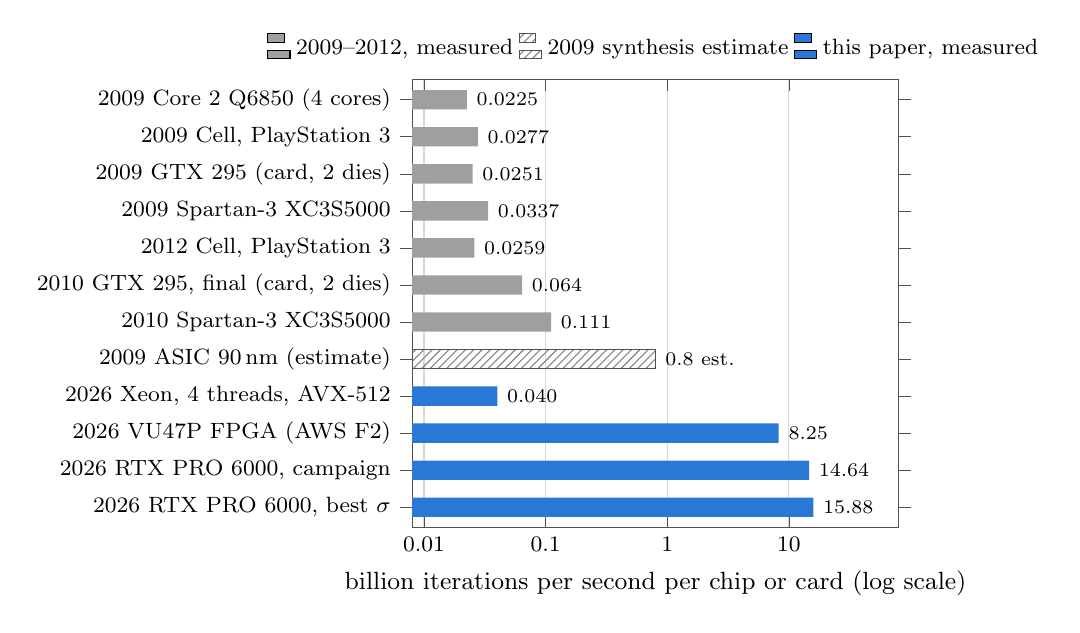
\begin{tikzpicture}
\begin{axis}[
  xbar, xmode=log, log basis x=10, log origin=infty,
  width=0.64\textwidth, height=0.6\textwidth,
  bar width=7pt, bar shift=0pt,
  xmin=0.008, xmax=80,
  xtick={0.01,0.1,1,10}, xticklabels={0.01,0.1,1,10},
  xlabel={billion iterations per second per chip or card (log scale)},
  symbolic y coords={core2,cell09,gtx09,sthreea,cell12,gtx10,sthreeb,asic,xeon,vu47p,pro6000c,pro6000b},
  ytick={core2,cell09,gtx09,sthreea,cell12,gtx10,sthreeb,asic,xeon,vu47p,pro6000c,pro6000b},
  yticklabels={
    {2009 Core 2 Q6850 (4 cores)},
    {2009 Cell, PlayStation 3},
    {2009 GTX 295 (card, 2 dies)},
    {2009 Spartan-3 XC3S5000},
    {2012 Cell, PlayStation 3},
    {2010 GTX 295, final (card, 2 dies)},
    {2010 Spartan-3 XC3S5000},
    {2009 ASIC 90\,nm (estimate)},
    {2026 Xeon, 4 threads, AVX-512},
    {2026 VU47P FPGA (AWS F2)},
    {2026 RTX PRO 6000, campaign},
    {2026 RTX PRO 6000, best $\sigma$},
  },
  y dir=reverse,
  xmajorgrids,
  enlarge y limits=0.05,
  nodes near coords,
  nodes near coords style={font=\scriptsize,color=black,anchor=west},
  point meta=explicit symbolic,
  legend style={at={(0.5,1.02)},anchor=south},
  legend columns=3,
  legend cell align=left,
]
\addplot[fill=inkS!55,draw=none] coordinates {
  (0.0225,core2) [0.0225] (0.0277,cell09) [0.0277] (0.0251,gtx09) [0.0251]
  (0.0337,sthreea) [0.0337] (0.0259,cell12) [0.0259] (0.064,gtx10) [0.064]
  (0.111,sthreeb) [0.111]};
\addlegendentry{2009--2012, measured}
\addplot[fill=white,draw=inkS,pattern=north east lines,pattern color=inkS!70] coordinates {(0.8,asic) [0.8 est.]};
\addlegendentry{2009 synthesis estimate}
\addplot[fill=cA,draw=none] coordinates {
  (0.040,xeon) [0.040] (8.25,vu47p) [8.25] (14.64,pro6000c) [14.64] (15.88,pro6000b) [15.88]};
\addlegendentry{this paper, measured}
\end{axis}
\end{tikzpicture}
\caption{ECC2K-130 rates, 2009--2012 against today, on one log scale
  (Tables~\ref{tab:history} and~\ref{tab:history-compare}). Each bar is
  one chip except the two GTX~295 bars, which are one card carrying two
  GPU dies, as their sources report them; per die they are half. One RTX~PRO~6000
  does the work of about 229 of the 2010 cards.}
\label{fig:history}
\end{figure}


\subsection{Comparison with today}
\label{sec:history-compare}

Table~\ref{tab:history-compare} sets the best 2009--2012 figure for
each platform class next to what we measured. All rows walk the same
classes of the same curve with the same $2^{60.9}$ budget; the 2009
walk and our campaign walk are the same map, and only the arithmetic
and the hardware differ.

\begin{table}[t]
\centering
\footnotesize
\caption{Best published rate per platform class against this paper's
  measurements, billions of iterations per second per chip. Ratios
  are ours. One year of $2^{60.9}$ iterations needs about $68.2$ billion
  iterations per second.}
\label{tab:history-compare}
\begin{tabular}{@{}llrlrr@{}}
\toprule
class & then & billion it/s & now & billion it/s & ratio \\
\midrule
GPU, per card & GTX 295 (2010) & 0.064 & RTX PRO 6000, campaign & 14.64 & $229\times$ \\
 & & & RTX PRO 6000, best $\sigma$ & 15.88 & $248\times$ \\
GPU, per die & GT200b (2010) & 0.032 & RTX PRO 6000 & 14.64 & $458\times$ \\
FPGA & Spartan-3 XC3S5000 (2010) & 0.111 & VU47P (AWS F2) & 8.25 & $74\times$ \\
ASIC & 90~nm estimate (2009) & 0.800 & --- & --- & --- \\
CPU, per core & Core 2, 3.0~GHz (2009) & 0.0056 & Xeon 2.1~GHz, AVX-512 & 0.0126 & $2.2\times$ \\
\bottomrule
\end{tabular}
\end{table}

The GPU row is the headline. One RTX~PRO~6000 running the campaign
build does the work of about 229 GTX~295 cards, and at that rate the
whole $2^{60.9}$ budget is about $4.7$ GPU-years instead of the 1{,}066
card-years of 2012. Of that factor, part is simply a bigger and faster
chip: 188 SMs at about $2.4$~GHz against 60 multiprocessors at
$1.24$~GHz is about $6\times$ more SM-clocks per second. The rest, roughly
$38\times$ per SM-clock, is the arithmetic: a native carry-less product
instead of a bitsliced one, three-input logic, a packed representation
with the Frobenius as a permutation network, and a batch shape tuned
against measured pipe rates. Figure~\ref{fig:gains} splits that factor, and Sections~\ref{sec:arith}
through~\ref{sec:gpu} take it apart step by step.

The FPGA gain is smaller, about $74\times$ from a 2010 Spartan-3 to a
current VU47P, and on cost per solve the F2 is level with the GPU
(Section~\ref{sec:fpga-vs-gpu}). The CPU gain per core is only about
$2\times$: the CPU client is the same bitsliced design as in 2009, and
it is the GPU that changed. The one platform class we have not
revisited is the ASIC. A 2009 synthesis estimate of $0.8$ billion
iterations per second per chip at 90~nm already needed fewer than a
hundred chips for a one-year solve; a modern node would need far
fewer, but that is a manufacturing question and outside this paper.

\section{Curve and field}
\label{sec:curve}

ECC2K-130 is the Certicom challenge~\cite{certicom1997}
\[
  E:\ y^2 + xy = x^3 + 1 \qquad\text{over }\FF_{2^{131}},
\]
a Koblitz curve~\cite{koblitz1992} defined over $\FF_2$, whose group
order is $4\cdot\ell$ with
\[
  \ell = 680564733841876926932320129493409985129,
\]
a 129-bit prime~\evcite{\evref{client}, ``The problems''}. The
challenge gives points $P$ and $Q$ of order $\ell$ and asks for $k$
with $Q=[k]P$. It has been open since 1997. The 2009 consortium
estimated the work at $2^{60.9}$ iterations of a
Frobenius-equivariant walk~\cite{bailey2009}, and
Section~\ref{sec:walk-constant} measures our walk at
$2^{60.91}$--$2^{60.92}$.

We did not take the curve on trust. $E(\FF_2)$ has four points, so
the Frobenius trace is $t=-1$, and the Koblitz recursion
$s_m = t\,s_{m-1} - 2 s_{m-2}$ gives $\#E(\FF_{2^{131}}) = 2^{131}+1-s_{131}
= 4\ell$. The \texttt{cryptanalysis} library's test suite checks the two facts that
pin down \emph{this} curve, on random points multiplied by the
cofactor: $\sigma^2+\sigma+2=0$, where $\sigma(x,y)=(x^2,y^2)$ is the
Frobenius, and $\ell\cdot
R=\mathcal{O}$~\evcite{\evref{cmodel}; \evref{cmodel}}.
Converting the published challenge point out of the normal basis gives
back Certicom's polynomial-basis hex, \texttt{05 1C99BFA6 F18DE467
C80C23B9 8C7994AA}~\evcite{\evref{client}, ``Validation''}.

\subsection{Normal basis}
\label{sec:onb}

Because $2\cdot131+1=263$ is prime and $2$ has order $131$ modulo
$263$, $\FF_{2^{131}}$ has a type-II optimal normal basis. Taking
$\zeta$ to be a primitive $263$rd root of unity, the basis is
$\gamma_i = \zeta^i + \zeta^{-i}$ for $i=1,\ldots,131$, and an element
is a 131-bit vector. Every design in this paper, on every platform,
leans on three consequences of that choice~\evcite{\evref{client}, ``Field representation''}.

\begin{center}
\small
\begin{tabular}{@{}p{0.42\textwidth}p{0.48\textwidth}@{}}
\toprule
fact & consequence \\
\midrule
$\gamma_i\gamma_j = \gamma_{i+j} + \gamma_{i-j}$
  (indices folded by $\gamma_{263-k}=\gamma_k$, $\gamma_0=0$)
  & a product is a cyclic convolution of two symmetric 263-bit
    vectors or, after a Bernstein--Lange change of basis, a
    polynomial product with no reduction step \\
$\gamma_i^2 = \gamma_{2i \bmod 263}$
  & squaring is the index permutation $i\mapsto\mathrm{fold}(2i)$,
    which is free in unrolled code and just wiring on an FPGA, so
    every Frobenius power $\sigma^k$ costs nothing \\
the Hamming weight of the vector is invariant under $\sigma$ and under
  negation $-(x,y)=(x,x+y)$
  & the iteration's branch selector and the distinguished-point test
    are functions on $\langle\sigma,-1\rangle$-classes that read the
    vector the hardware already holds \\
\bottomrule
\end{tabular}
\end{center}

\subsection{Reference model}
\label{sec:golden}

The code generator models the field as symmetric vectors over
$\ZZ/263\ZZ$ modulo the all-ones vector, with multiplication as
cyclic convolution. That model is complete and simple enough to verify by inspection, and
every generated routine is checked against it on 64 random inputs
before it is written out~\evcite{\evref{codegen}; \evref{codegen}}.
The bitsliced multiply, square, inverse, $\sigma^7$ and Hamming weight
are also tested differentially against a reference implementation
that shares no code with them. We check that the iteration function
commutes with Frobenius and with negation, that the collision solver
recovers a planted logarithm, and that the distinguished-point
comparison is right for every weight and cutoff. In all,
\texttt{make test} runs 52 such checks across
$\mathrm{GF}(2^{23})$, $\mathrm{GF}(2^{41})$, $\mathrm{GF}(2^{83})$ and
$\mathrm{GF}(2^{131})$~\evcite{\evref{client}, ``Validation''}.

The same model is the oracle for every other platform. The VHDL
engine's reference script imports it directly and uses it to prove the
basis-change maps, the multiplier route, $\sigma^j$, the inversion
chain and a full step before it emits test vectors
(Section~\ref{sec:fpga})~\evcite{\evref{hdl}}. The \texttt{cryptanalysis}
library's C model of the same field and curve
\evcite{\evref{cmodel}} was written separately
and re-walks every GPU report that library imports. When the two
models agree on a record, they agree on the exact 131-bit vector in
the same permuted basis, not merely up to a change of
basis~\cite{ecdlppaper}.

Longer runs exercise the reporting path rather than the algebra. On
$\mathrm{GF}(2^{83})$, $12.6$~M iterations produced 172 distinguished
points, within $30\%$ of the predicted rate, and the reference
recomputed 60 of them from their seeds without a mismatch, including
walks that had been restarted. On the challenge curve itself, with the
cutoff loosened from 34 to 50 so that points actually appear, $3.1$~M
iterations produced $12{,}368$ reports, and the 25 we recomputed all
matched exactly~\evcite{\evref{client}, ``Validation''}.

\subsection{ECC2K-95}
\label{sec:ecc2k95}

ECC2K-95 is the retired Certicom challenge on the same curve equation
over $\FF_{2^{97}} = \FF_2[t]/(t^{97}+t^6+1)$, with group order $4\ell$
for the 95-bit prime $\ell = 39614081257132074233778707191$. Harley and
collaborators solved it in 1998~\cite{harley1998}. Since $2\cdot97+1=195$
is composite there is no type-II optimal normal basis, so the client
runs a polynomial-basis backend and computes the orbit-invariant
weight through one generated linear map into a normal basis, which is
how Harley's own client did it~\evcite{\evref{client}, ``ECC2K-130 and ECC2K-95''}.

We recovered the parameters from Harley's surviving client source.
The generator refuses to emit the curve unless both points lie on it,
both have order $\ell$, and the published answer
\[
  k = 37837308472231540269443981458
\]
satisfies $[k]P=Q$. The expected work is about $2^{44}$ iterations.
Harley's group measured $2.16\cdot10^{13}$, against the
$1.79\cdot10^{13}$ that this walk predicts from
$\sqrt{\pi\ell/(4m)}$~\evcite{\evref{client}, ``The problems''}. Per
iteration the polynomial-basis field is about $1.9\times$ cheaper than
$\mathrm{GF}(2^{131})$ in the normal basis (roughly $32{,}000$ against
$60{,}000$ bitsliced instructions). That makes ECC2K-95 a job of a few
GPU-hours where ECC2K-130 takes GPU-centuries, which is exactly what an
end-to-end test of the whole pipeline needs: the same machinery at a
scale that finishes~\evcite{\evref{client}, ``ECC2K-95''}. The
repository's separate ECC2K-95 CUDA kernel has so far run only under
CPU emulation, where it recovers 21-bit and 40-bit toy logarithms at
$0.94\times$ and $1.32\times$ its own prediction; we do not use it for
any throughput claim~\evcite{\evref{ecc2k95}}.

\section{Walks}
\label{sec:walk}

Pollard's rho~\cite{pollard1978}, in the parallel collision-search
form of van Oorschot and Wiener~\cite{vanoorschot1999}, runs many
pseudo-random trails through the group, reports the distinguished
points they pass, and solves the logarithm when two trails meet. On a
Koblitz curve the Frobenius $\sigma$ and negation generate a group of
$2m=262$ automorphisms acting on $\langle P\rangle$. A walk defined on
the orbits of that group needs $\sqrt{262}\approx16.2$ times fewer
steps~\cite{wienerzuccherato1998,glv2000,duursma1999}. With
$N=(\ell-1)/262$ classes, the expected number of classes visited
before a collision is $\sqrt{\pi N/2}$, which here is
$2^{60.809}$~\evcite{\evref{walkconst}, §1}. Every walk in this
paper is a map on those classes. They differ in how they respect the
class action and in what each step costs.

\subsection{$\sigma$-walk}
\label{sec:walk-sigma}

The campaign uses the map of Bailey et al.~\cite{bailey2009}:
\begin{align*}
  j &= 3 + \bigl((\HW(x_R) \gg 1) \bmod 8\bigr) \in [3,10],\\
  R' &= \sigma^j(R) + R,\\
  \text{distinguished} &\iff \HW(x_R)\le w,
\end{align*}
with $w=34$ by default in the client and $w=32$ in the live campaign.
Because the weight is a class invariant, $f(\sigma R)=\sigma f(R)$ and
$f(-R)=-f(R)$, so the map descends to classes without ever computing a
canonical representative inside the loop. The division by two in the
selector matters more than it looks: $x$-coordinates of subgroup
points always have even weight, so a selector on the raw weight would
only ever use four of the eight branches~\evcite{\evref{ecc2k95}}.

One step is one affine addition, with the inversion shared across a
batch (Section~\ref{sec:arith}). In the normal basis $\sigma^j$ is an
index permutation and costs nothing. As a scalar, the step is
$R\mapsto[1+s^j]R$, where $s$ is the root of $s^2+s+2=0$ that $\sigma$
realises on $\langle P\rangle$. Selecting $\sigma^j$ needs no branch:
it is three conditional squarings, each a single \texttt{LOP3} per
word, and $j$ itself is never materialised~\evcite{\evref{client}, ``Iteration function''}.

The walk tracks no coefficients. A walk is identified by its seed, and
a report is the pair (seed, canonical endpoint), 32 bytes in all. The
start point is $R_0 = Q + \sum_i c_i\,\sigma^i(P)$, where $c$ is a
128-bit string from a PRF of the seed. It is computed with the same
arithmetic and merged into finished lanes under a mask. Tracking a
linear combination inside the loop would cost a 129-bit modular
multiplication per step, which this walk cannot afford. Instead,
collision resolution re-walks both trails and counts how often each
branch $1+s^j$ was applied. That gives
$\text{endpoint} = [\mu](\alpha_0 P + Q)$ with $\mu=\prod_j(1+s^j)^{n_j}$;
the solver matches the two endpoints up to Frobenius and negation and
solves for $k$ modulo $\ell$~\evcite{\evref{client}, ``Distinguished points and restarts''}.
The $\sigma$-walk has no fruitless cycles: no product
$\prod_j(1+s^j)^{n_j}$ equals $\pm s^a$, so a trail can never come back
to its own class~\evcite{\evref{walkconst}, §5}.

The client can optionally carry the eight branch counters as it goes
(\texttt{WITNESS=1}). Because $\mu$ is a commuting product, that is
just eight counters and nothing is multiplied per step. The payoff is
that a third party can check a report with one scalar multiplication
$[\mu]R_0$, 196 point operations, instead of re-walking the
$2^{25.27}$ steps that a weight-34 report represents, an asymmetry of
about $2^{17.7}$. On the bitsliced CPU walk this costs $6.0\%$, the
median of three paired rounds ($40.026$ to $37.762$~million iterations/s, a $5.7\%$
drop in rate, against $33.8\%$ predicted; an earlier revision measured
$4.2\%$ on a pre-merge tree). On the packed GPU walk the rate fell
$34.7\%$, from $14.003$ to $9.150$~billion iterations/s. That figure is stated in the
note, but only its job script was frozen with the
record. Either way it is far above the
$2\%$ the note had set as its threshold for abandoning a 16-bit
counter layout that was never built, so the campaign builds pin
\texttt{WITNESS=0} and the record stays at 32
bytes~\evcite{\evref{witness}; \evref{ops}}.
A later fused kernel narrows the packed cost ($9.347867$ to
$11.800903$~billion iterations/s in witness-carrying mode) but does not close
it~\evcite{\evref{sigmafused}}.

\subsection{Table walk}
\label{sec:walk-table}

On a GPU, the $\sigma$-walk pays for $\sigma^j$ in the basis
conversions around it (Section~\ref{sec:arith-packed}). An $r$-adding
walk on the same classes avoids that cost:
\begin{align*}
  h(R) &= (\HW(x)/2) \bmod 8,\\
  k(R) &= \Bigl(\textstyle\sum_e L(e)\,x_e\Bigr)\cdot \HW(x)^{-1} \bmod 131,\\
  \varepsilon(R) &= \text{bit $p(R)$ of } y,\\
  R' &= R + (-1)^{\varepsilon}\,\sigma^{k}(T_h),
\end{align*}
where $T_h=[a_h]P+[b_h]Q$ and the $131\times8$-point table lives in
shared memory ($37.7$~KB, or $48.5$~KB per block with the selection
tables). Since $k$ shifts by one under $\sigma$ and $\varepsilon$ flips
under negation, the walk descends to classes. Each step is one affine
addition with a table operand whose Frobenius power is a lookup
rather than a conversion~\evcite{\evref{iterfn}, §4 and §6.1}.

Unlike the $\sigma$-walk, an adding walk on classes does have
fruitless cycles~\cite{bls2011}. Two kinds show up here: four-step
patterns in which the table points' Frobenius powers satisfy a
relation coming from $\tau^2+\tau+2=0$, and six-step pairwise patterns.
The first cycle rule let 24 four-step and 4 six-step patterns through.
Observed against predicted counts were $1{,}145$ against $1{,}312$
($0.87\pm0.03$) for the $\tau$-relation class and 126 against 166 for
the pairwise class~\evcite{\evref{walkconst}, §5}. At the
campaign's trail length of $2^{28.41}$ steps, a model built on those
measured rates predicts that the cycles trap $53.7\%$ of trails, a
loss of $7.1$--$8.6\times$ with the $2^{30}$ iteration
guard~\evcite{\evref{walkconst}, §6}. A revised rule (v2) brings
residual trapping down to $2.0\cdot10^{-5}$ of trails, at a
$1.0048\times$ iteration cost from merge parting. A third revision (v3,
Section~\ref{sec:walk-cycles}) replaces the history-dependent exits
with a raw-cycle anchor~\evcite{\evref{walkconst}, §11.1}.

\subsection{Bridge map}
\label{sec:walk-bridge}

On the power-capped RTX~PRO~4500 a third map turns out to pay. Its
common transition is $R' = R + \sigma(R)$, which is the scalar $[1+s]$.
On this curve $x(R+\sigma R)=x+1/x$, the square root of $x([2]R)$, so
the walk can keep an $x$-only state. That scalar on its own generates
a subgroup of index 12, so the map takes a sparse bridge
$R' = R + \sigma^3(R)$ (index 109 on its own) whenever
$\HW(x) \bmod 72 = 14$. Together the two transitions generate the full
group, which the earlier $[2]/[3]$ map had failed to do by an index of
two (we called it ``the scalar subgroup defect'')~\evcite{\evref{client}, ``ECC2K-130 and ECC2K-95''}.
We froze a study of $2{,}000$ trials on $\mathrm{GF}(2^{23})$, where the
modulus-72 bridge predicate selects exactly what the earlier modulus-32
one did (weight 14 only). It gives mean charged work of
$1.006696\times$ that of the map selected at the time, so the new map's
throughput gain (Section~\ref{sec:g7}) is not given back in extra
iterations. The map also passes an independent $2{,}048$-point affine
checkpoint~\evcite{\evref{bridge}}.

\subsection{Walk constant}
\label{sec:walk-constant}

Throughput is only half of what determines how long a solve takes.
The other half is how many iterations the walk needs, which for a
non-random map differs from the random-mapping $\sqrt{\pi N/2}$ by a
constant $c$. We measure $c$ as iterations divided by a random
mapping's iterations on the class set, on small Koblitz curves of the
same family. The device walk and a host emulation are measured
separately, with an $r$-adding control using 256 branches alongside~\evcite{\evref{walkconst}, §4}.

\begin{table}[t]
\centering
\small
\caption{Walk constant $c$ on toy Koblitz curves, ECC2K-130 branch
  distribution ($H=8$). Floor $c=1$. The adding-walk control with 256
  branches measures $1.0002\pm0.0012$ at $n=23$. The injective-branch
  model $1/\sqrt{1-\sum p^2}$ predicts $1.070$ for the $\sigma$-walk
  at $n=131$.}
\label{tab:walkconst}
\begin{tabular}{@{}rlll@{}}
\toprule
$n$ & measured on & table walk & $\sigma$-walk \\
\midrule
23 & host emulation & $1.0037\pm0.0012$ & $1.0995\pm0.0013$ \\
23 & device & $1.0076\pm0.0037$ & $1.0948\pm0.0040$ \\
31 & host emulation & $1.0035$ & $1.0964$ \\
37 & host emulation ($W=16$) & $1.0036$ & $1.0949$ \\
41 & host emulation & $1.0125\pm0.0059$ & $1.0910\pm0.0064$ \\
41 & device & $1.0051\pm0.0299$ & $1.0997\pm0.0336$ \\
59 & host emulation & $0.9949$ & $1.0817$ \\
\midrule
\multicolumn{2}{@{}l}{pooled / extrapolated to $n=131$} & $1.0035\pm0.0006$ & $[1.070,\,1.082]$ \\
\bottomrule
\end{tabular}
\end{table}

The $\sigma$-walk is one-to-one on each branch, so it pays the
injective-branch penalty $1/\sqrt{1-\sum_j p_j^2}$. With the weight
distribution at $n=131$ ($\sum p_j^2=0.127$) that penalty is $1.070$.
The measurements in Table~\ref{tab:walkconst} drift from $1.0995$ at
$n=23$ toward it, and extrapolate to $[1.070,1.082]$ at $n=131$. The
table walk is not injective per branch and sits at $1.0035\pm0.0006$
pooled, so the ratio $c_t/c_\sigma$ is $0.928$--$0.938$. The expected
work for the campaign's $\sigma$-walk is therefore
\[
  2^{60.809}\times[1.070,\,1.082] = 2^{60.91}\text{--}2^{60.92}
\]
iterations. Under the original $2^{30}$ restart guard it would be a
further $1.185\times$ ($2^{61.15}$--$2^{61.17}$): a guard at three trail
lengths cuts the longest $4.9\%$ of trails and so throws away $15.6\%$
of the steps (again a model on the measured rates). Bailey et al.'s
$2^{60.9}$ holds up~\evcite{\evref{walkconst}, §6}. The guard has
since been raised to $2^{32}$, twelve trail lengths at weight 32,
which discards only $0.007\%$ of steps ($1.00007\times$)~\evcite{\evref{maxiters}}.

As a direct check, on $\mathrm{GF}(2^{41})$ with 128 walks, cutoff 13
and 64 planted logarithms, the $\sigma$-walk needed
$164{,}200\pm9{,}900$ iterations per solve and the table walk
$157{,}800\pm7{,}500$, a ratio of $0.96\pm0.07$. The bare prediction is
$102{,}600$; the difference is roughly $1.5\times$ of harness overhead
from the distinguished-point tail~\evcite{\evref{iterfn}, §6.2}.

\subsection{Cost per solve}
\label{sec:walk-cycles}

Put rate and constant together and the table walk looks very
different. Its throughput advantage (Section~\ref{sec:tablewalk}) is
$1.09$--$1.15\times$ and its walk constant is $0.93\times$. But its
as-built cycle rule is modelled to trap half of all campaign-length
trails, so the as-built kernel's cost per solve was $4.85$--$6.26\times$
that of the $\sigma$-walk. With rule v2 the projection improves to
$0.81$--$0.86\times$, and the switch deadline, the fraction of the
campaign after which switching no longer pays, is $15$--$22\%$. That
projection is untested: the note declares the paired rate measurement
for the v2 kernel that would test it, and it has not been
run~\evcite{\evref{walkconst}, §11}. So the campaign still walks
the $\sigma$-map, and the $20$~billion iterations/s table-walk rows in
Section~\ref{sec:tablewalk} are rates, not costs per solve.

Rule v2 itself refused all $19{,}200$ $\tau$-cycles in a dedicated
test, passed a $4{,}096$-point host probe without a mismatch, solved
$8/8$ planted logarithms, and its scatter check against the predicted
cycle counts gives $\chi^2=8.79$ on 15 degrees of freedom (the v1 rule
gives $23.30$)~\evcite{\evref{walkconst}, §11.1 and §11.6.1}. Rule
v3 then replaced the history-dependent exits with a raw-cycle probe of
at most eight steps and a least-key anchor exit. It is checked by
regression tests on a raw two-cycle found on the challenge curve and
on synthetic entry-phase cycles, with $300$ of $300$ device reports
re-walked and identical corpora across arms. V2's walk-constant and
throughput figures do not carry over to it, and the exact v3 kernel
currently runs at about half of the $\sigma$-walk's rate
(Section~\ref{sec:sigma-vs-table})~\evcite{\evref{v3}}.
V3 needs a new table corpus; the campaign's $\sigma$-walk corpus is
unaffected.

\section{Field arithmetic}
\label{sec:arith}

Field multiplication dominates a step. The addition itself needs two
products. With $W$ walks sharing one inversion through Montgomery's
trick~\cite{montgomery1987}, the product tree adds $3(W-1)/W$ more,
plus $1/W$ of an Itoh--Tsujii inversion~\cite{itoh1988}, which costs
only eight multiplications in a basis where squaring is free (the
client's addition chain is $1,2,4,8,16,32,64,65,130$; the FPGA's is
$1,2,4,\ldots,128,130$)~\evcite{\evref{packedsrc}; \evref{hdl}}.
Going from $W=4$ to $W=32$ is worth $60\%$ on the CPU client, because
it shrinks the amortised inversion from $25\%$ to $3\%$ of the
multiplication budget~\evcite{\evref{client}, ``Throughput''}. How a
multiplication is represented is therefore the central design
decision, and the repository carries two answers.

\subsection{Bitsliced}
\label{sec:arith-bitsliced}

The original client is bitsliced in Biham's sense~\cite{biham1997}:
one word operation advances $W$ walks at once, one per bit lane, and a
field operation is a straight-line program of word-wide Boolean
instructions generated from the field model. The GPU uses 32-bit
words. The host uses the widest it has (512 lanes with AVX-512, 256
with AVX2, 128 with NEON), and the arithmetic source is identical at
every width~\evcite{\evref{client}, ``Word width''}.

Multiplication follows Bernstein and Lange~\cite{bernsteinlange2010onb}.
Both operands are converted from the normal basis to the optimal
polynomial basis $\{1,c,c^2,\ldots\}$ with $c=\gamma_1$, multiplied as
polynomials, and the 261-coefficient product is converted back. We
generate both conversions from the substitution $c=z+1/z$, which
splits by parity as
$H(c)=H_{\mathrm{even}}(c^2)+c\,H_{\mathrm{odd}}(c^2)$; because squaring
is an index permutation, this yields an $O(K\log K)$ conversion. The
generated \texttt{multPrep} is 331 instructions and the double-size
inverse conversion 903, against 325 and 909 for the hand-designed
chains in the literature~\evcite{\evref{client}, ``Findings''}.

This backend taught us two things that change the usual accounting.
The first is that three-input logic fusion (\texttt{LOP3} on NVIDIA,
\texttt{vpternlogd} on AVX-512, \texttt{BSL}/\texttt{EOR3} on Arm with
\texttt{FEAT\_SHA3}) is worth $1.65\times$. A 131-bit multiplication is
$14{,}554$ two-input bit operations but only $8{,}859$ instructions
once $x\oplus y\oplus z$ and $x\oplus(y\wedge z)$ are single
instructions. Since the fused form makes the XOR that accompanies an
AND free, schoolbook leaves beat Karatsuba leaves~\cite{karatsuba1962}:
full recursion costs $18{,}819$ bit operations and $14{,}770$
instructions, while stopping at a 17-bit schoolbook leaf costs more
bit operations but fewer instructions. A search over balanced and
unbalanced splits found nothing below $8{,}859$. Toom-3 over $\FF_2$,
the source of Bernstein's $11{,}961$-bit-operation
chain~\cite{bernstein2009batch}, is not
implemented~\evcite{\evref{client}, ``What is not done''}. The second
lesson is that code size, not arithmetic, is the real wall. Inlining
everything produced $285{,}096$ PTX instructions for one kernel, and
\texttt{ptxas} had still not finished register allocation after five
minutes. Turning the multiplication, inversion, conversions, leaf,
weight tree and $\sigma^j$ into real subroutines brought it down to
$36{,}553$ lines and a $2.4$~s assembly~\evcite{\evref{client}, ``Findings''}.

The Hamming-weight tree is 268 instructions against 654 bit
operations, because a full adder is two \texttt{LOP3}s. The whole
bitsliced iteration comes to about $60{,}000$ instructions per 32
walks on $\mathrm{GF}(2^{131})$, as a static count. On the GPU that is
the $0.85$~billion iterations/s control of Section~\ref{sec:ledger}. For comparison,
the instruction-count ceiling of the later packed kernel on the
RTX~PRO~6000 is $17.6$~billion iterations/s ($27.1$~T lane-operations/s over about
$1{,}540$ lane-operations per update, a different
count)~\evcite{\evref{ceiling}}.

\subsection{Packed}
\label{sec:arith-packed}

The packed backend holds one walk's coordinates in five 32-bit words
per thread and multiplies with carry-less
instructions~\evcite{\evref{packed}}. Coordinates live in
$\FF_2[c]/(m)$ with $c=\gamma_1$, so a 131-bit product is a Karatsuba
over carry-less multiplies (six \texttt{CLMAD}) followed by a
reduction~\evcite{\evref{iterfn}, §1}. The normal basis,
where the weight, branch selection and distinguished-point test live,
is reached through the same Bernstein--Lange conversions, implemented
as shift-and-mask networks and, for the Frobenius powers, as
Bene\v{s} permutation networks~\evcite{\evref{frobnet}}.
Before CUDA~13.3 the carry-less product had to be built from integer
multiplies. The native \texttt{clmad.lo}/\texttt{hi} instructions that
PTX~9.3 exposes for \texttt{sm\_80} and later were worth $+22.4\%$ on
the RTX~PRO~6000 (Section~\ref{sec:ledger}), and they are why the
campaign preset requires that compiler;
Section~\ref{sec:blackwell-clmad} describes the instruction and its
very different rates across parts~\evcite{\evref{clmad}}.

The natural unit of account changes with the representation. In the
packed kernel the shipping walk issues $4.81$ products per update at
batch 16 and about $2{,}324$ static ALU
slots~\evcite{\evref{iterfn}, §1 and §3}. The count that
matters is \texttt{CLMAD}s, and Section~\ref{sec:floor} prices it.
The reduction \texttt{reducePolynomial131} alone is $440.6$
lane-instructions per update, $29\%$ of the integer work of the
$20$~billion iterations/s build~\evcite{\evref{roofline}}.

\begin{figure}[t]
\centering
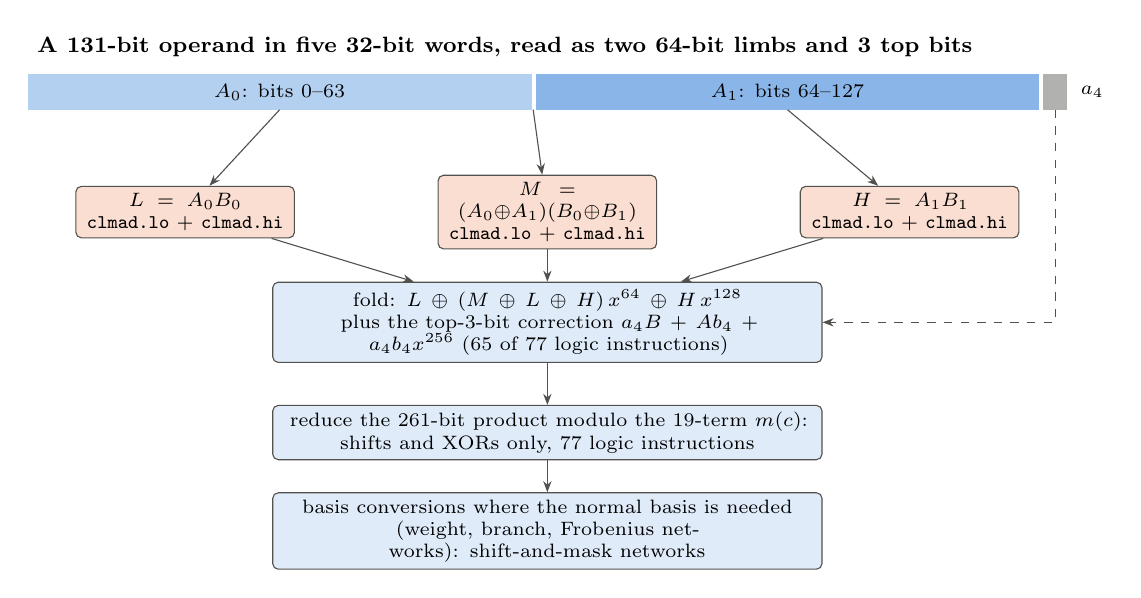
\begin{tikzpicture}[
  font=\scriptsize,
  arr/.style={-{Stealth[length=4pt]},inkS},
  leaf/.style={draw=inkS,rounded corners=2pt,fill=cB!22,align=center,inner sep=2.5pt,text width=2.6cm},
  alu/.style={draw=inkS,rounded corners=2pt,fill=cA!15,align=center,inner sep=2.5pt},
]
% operand
\node[anchor=west,font=\footnotesize\bfseries] at (0,4.35) {A 131-bit operand in five 32-bit words, read as two 64-bit limbs and 3 top bits};
\fill[cA!35] (0,3.55) rectangle (6.4,4.0);  \node at (3.2,3.775) {$A_0$: bits 0--63};
\fill[cA!55] (6.45,3.55) rectangle (12.85,4.0); \node at (9.65,3.775) {$A_1$: bits 64--127};
\fill[inkS!45] (12.9,3.55) rectangle (13.2,4.0); \node[anchor=west] at (13.25,3.775) {$a_4$};
% leaves
\node[leaf] (L) at (2.0,2.25) {$L=A_0B_0$\\\texttt{clmad.lo} + \texttt{clmad.hi}};
\node[leaf] (M) at (6.6,2.25) {$M=(A_0{\oplus}A_1)(B_0{\oplus}B_1)$\\\texttt{clmad.lo} + \texttt{clmad.hi}};
\node[leaf] (H) at (11.2,2.25) {$H=A_1B_1$\\\texttt{clmad.lo} + \texttt{clmad.hi}};
\draw[arr] (3.2,3.55) -- (L); \draw[arr] (6.42,3.55) -- (M); \draw[arr] (9.65,3.55) -- (H);
% fold
\node[alu,text width=6.8cm] (F) at (6.6,0.85) {fold: $L \oplus (M\oplus L\oplus H)\,x^{64} \oplus H\,x^{128}$\\
  plus the top-3-bit correction $a_4B + Ab_4 + a_4b_4x^{256}$ (65 of 77 logic instructions)};
\draw[arr] (L) -- (F); \draw[arr] (M) -- (F); \draw[arr] (H) -- (F);
\draw[arr,dashed] (13.05,3.55) -- (13.05,0.85) -- (F.east);
% reduction
\node[alu,text width=6.8cm] (R) at (6.6,-0.55) {reduce the 261-bit product modulo the 19-term $m(c)$:\\shifts and XORs only, 77 logic instructions};
\draw[arr] (F) -- (R);
\node[alu,text width=6.8cm] (C) at (6.6,-1.8) {basis conversions where the normal basis is needed\\(weight, branch, Frobenius networks): shift-and-mask networks};
\draw[arr] (R) -- (C);
\end{tikzpicture}
\caption{The packed 131-bit product. Three $64\times64$ carry-less leaves
  (six \texttt{CLMAD} instructions) form a one-level Karatsuba; the three
  top bits, the fold, the reduction and every basis change run on the
  logic pipe. On the RTX~PRO~6000 a \texttt{CLMAD} costs the issue time of
  $37.8$ logic instructions, so the split keeps only the six leaf products
  on the carry-less unit; on a B200 or H100, where it costs $2$--$3.8$,
  moving the correction and even the reduction onto \texttt{CLMAD} pays
  instead (Section~\ref{sec:blackwell-rates}).}
\label{fig:clmad}
\end{figure}


\subsection{Cross-validation}
\label{sec:arith-compat}

The two backends, the CPU client at every word width, the VHDL engine
and the \texttt{cryptanalysis} library's imported kernel all stay bit-for-bit
compatible. A distinguished-point record written by any of them
re-walks under any other, and every GPU report is re-walked on the
host reference before we record a rate. The host check re-slices
packed words into the same permuted type-II basis and compares
vectors, not classes~\evcite{\evref{client}, ``Validation''}. One
corner case is worth mentioning. When $\sigma^j(R)=\pm R$, the
addition's denominator is zero; this happens with probability about
$2^{-131}$ per step. The $\sigma$-walk client and the VHDL engine do
not special-case it. A zero denominator inverts to zero, the batch's
points become garbage, and the next distinguished-point check or the
iteration guard throws them away. The \texttt{cryptanalysis} C model and the table
walk abort the step instead~\evcite{\evref{refsrc}; \evref{hdl}}.

\section{Instruction sets}
\label{sec:isa}

Pollard rho on these curves needs two kinds of arithmetic: products of
binary polynomials (for $\FF_{2^{131}}$) and multi-word integer products
with long carry chains (for the NIST primes). Both have gained dedicated
instructions over the last fifteen years, on GPUs and CPUs alike.
Table~\ref{tab:isa} and Figure~\ref{fig:isa} summarise the ones this
paper uses or prices; the rest of this section says why each matters.

\begin{table}[t]
\centering
\footnotesize
\setlength{\tabcolsep}{4pt}
\caption{Instructions relevant to rho on $\FF_{2^{131}}$ and on prime
  fields, with the first generation that has each. ``Use here'' says how
  this paper's code uses it: in the measured clients, priced, or not
  yet tried.}
\label{tab:isa}
\begin{tabular}{@{}p{0.2\textwidth}p{0.31\textwidth}p{0.2\textwidth}p{0.2\textwidth}@{}}
\toprule
instruction & what it does & first available & use here \\
\midrule
\multicolumn{4}{@{}l}{\emph{NVIDIA GPUs}} \\
\texttt{PRMT}, \texttt{POPC}, \texttt{FLO} & byte permute; population count; find leading one & Fermi (2010) & every client \\
\texttt{SHF} & funnel shift of a register pair & Kepler (2012--13) & every client \\
\texttt{LOP3} & any 3-input Boolean function & Maxwell (2014) & every client \\
\texttt{IADD3}, native \texttt{IMAD} & 3-input add; 32-bit multiply-add & Maxwell; Volta (2017) & NIST walk \\
\texttt{mad.lo.cc}, \texttt{madc.hi.cc} & multiply-add with carry in/out (PTX) & all CUDA GPUs & NIST walk \\
\texttt{clmad.lo}/\texttt{.hi} & $64{\times}64$ carry-less multiply-add (PTX 9.3) & CUDA 13.3 (2026), \texttt{sm\_80}+ & ECC2K-130 client \\
\midrule
\multicolumn{4}{@{}l}{\emph{x86 (Intel, AMD)}} \\
\texttt{PCLMULQDQ} & $64{\times}64$ carry-less multiply & Westmere (2010) & packed CPU client \\
\texttt{MULX}, \texttt{ADCX}/\texttt{ADOX} & flag-free multiply; two carry chains & Haswell (2013); Broadwell (2014) & not tried \\
\texttt{VPTERNLOGD} & any 3-input Boolean function, 512-bit & Skylake-SP (2017) & bitsliced client \\
\texttt{VPMADD52} (IFMA) & $52{\times}52$-bit multiply-add & Cannon Lake (2018) & not tried \\
\texttt{VPCLMULQDQ}, GFNI & 4 carry-less products per 512 bits; GF($2^8$) affine & Ice Lake (2019); AMD Zen 4 (2022) & priced \\
\midrule
\multicolumn{4}{@{}l}{\emph{Arm}} \\
\texttt{PMULL}/\texttt{PMULL2} & $64{\times}64$ carry-less multiply & Armv8.0 Crypto & packed CPU client \\
\texttt{EOR3}, \texttt{BCAX} & 3-way XOR; AND-NOT then XOR & Armv8.2 SHA3 & bitsliced client \\
SVE2 \texttt{PMULLB/T}, \texttt{EOR3} & vector carry-less and 3-input logic & Armv9.0 (SVE2-AES) & not tried \\
\midrule
\multicolumn{4}{@{}l}{\emph{RISC-V}} \\
Zbc, Zvbc & scalar and vector carry-less multiply & ratified 2021, 2023 & not tried \\
\bottomrule
\end{tabular}
\end{table}

\paragraph{NVIDIA GPUs.} The integer pipe has grown three instructions
that a binary field uses on every step. \texttt{PRMT} and \texttt{POPC}
date from Fermi, the funnel shift \texttt{SHF} from Kepler, and
\texttt{LOP3}, which evaluates any Boolean function of three inputs from an
8-bit truth table, from Maxwell~\cite{nvidia_binutils}. \texttt{LOP3}
alone is worth $1.65\times$ on the bitsliced product
(Section~\ref{sec:arith-bitsliced}). \texttt{POPC} still issues at a
quarter of the logic rate on every current part, 16 per clock per SM, so
each Hamming weight costs about four logic slots~\cite{nvidia_bpg134}.
The prime-field side relies on PTX's carry-chain forms, which every CUDA
GPU has; the extended-precision forms issue at half the rate of a plain
multiply-add~\cite{nvidia_bpg134}.

The change that matters most for ECC2K-130 is recent. PTX ISA~9.3,
shipped with CUDA~13.3 in May 2026, added \texttt{clmad.lo} and
\texttt{clmad.hi}: the low and high halves of a $64\times64$ carry-less
product, XORed into an addend, for \texttt{sm\_80} and
later~\cite{nvidia_ptx93}. NVIDIA describes it as accelerated in hardware
since Ampere and reports GHASH at about 6.3~TB/s on a B200 and 1.3~TB/s
on an RTX~5090~\cite{watson2026clmad}. NVIDIA documents neither its SASS
mnemonic nor its issue rate, which is why we measured both
(Section~\ref{sec:blackwell-rates}). Nsight attributes it to the FP64
pipe, and it is slow exactly where FP64 is slow: about two lanes per
SM-clock on the RTX~PRO~6000, ten to eighteen times that on the B200 and
H100. That matters because
NVIDIA's FP64 ratio varies by product rather than by generation: $2{:}1$
against FP32 on the A100, H100 and B200, but $64{:}1$ on the GA10x and Ada
consumer parts, on the RTX~PRO~6000 and on the
B300~\cite{nvidia_ga102_wp,nvidia_ada_wp,nvidia_h100_wp,nvidia_rtx_blackwell_wp,aubrey2025blackwellultra}.

Two other generational changes show up in our rates. From Ampere's GA10x
parts onward each SM partition pairs 16 FP32-only lanes with 16 lanes that
do FP32 or INT32, and Ada kept that split; the workstation Blackwell
chips (\texttt{sm\_120}) unify them, so every lane can issue integer
work~\cite{nvidia_ga102_wp,nvidia_ada_wp,nvidia_rtx_blackwell_wp}. That is
consistent with the factor of two we measure per SM between Ada and
\texttt{sm\_120} on this integer-bound walk (Section~\ref{sec:blackwell-logic}).
Hopper's DPX instructions (fused add with min or max for dynamic
programming), its tensor memory accelerator and Blackwell's
\texttt{tcgen05} tensor-memory instructions do not help this walk; the
products here have no operand shared across lanes, which tensor cores
need (Section~\ref{sec:open-method}).

\paragraph{x86.} Intel added \texttt{PCLMULQDQ} with Westmere in
2010~\cite{gueron2014clmul}, \texttt{MULX} with Haswell and the dual carry
chains \texttt{ADCX}/\texttt{ADOX} with Broadwell~\cite{ozturk2012adx},
AVX-512 with its ternary-logic \texttt{VPTERNLOGD} in Skylake-SP, the
52-bit integer multiply-add IFMA in Cannon Lake~\cite{gueron2016ifma}, and
the 512-bit \texttt{VPCLMULQDQ} (four carry-less products per instruction)
with GFNI in Ice Lake~\cite{intel_sdm_vol1,drucker2018vpclmulqdq}. AMD
implemented AVX-512, including \texttt{VPCLMULQDQ} and GFNI, in Zen~4 on a
256-bit datapath that issues each 512-bit operation in two halves, and
Zen~5's server parts run it at full width~\cite{amd_58003,amd_epyc5_wp}.
Intel's AVX10.2 makes 512-bit vectors universal and APX doubles the
general-purpose registers to 32~\cite{intel_avx102,intel_apx}; both would
help a register-starved bitsliced leaf (Section~\ref{sec:cpu-bitsliced}).

\paragraph{Arm and RISC-V.} Armv8.0's optional Crypto extension has the
$64\times64$ carry-less \texttt{PMULL}; the Armv8.2 SHA3 extension adds the
three-input \texttt{EOR3} and \texttt{BCAX}; SVE2 brings vector forms of
both, with 128-bit-result \texttt{PMULLB}/\texttt{PMULLT} in the SVE2-AES
extension~\cite{arm_a64_2026}. Graviton2 (Neoverse N1) has PMULL but not
SHA3, Graviton3 (V1) adds SHA3 and SVE, and Graviton4 (V2) has SVE2 with
the 128-bit PMULL.
RISC-V ratified scalar carry-less multiply (Zbc) in 2021 and its vector
form (Zvbc) in 2023~\cite{riscv_bitmanip,riscv_vcrypto}.

\begin{figure}[t]
\centering
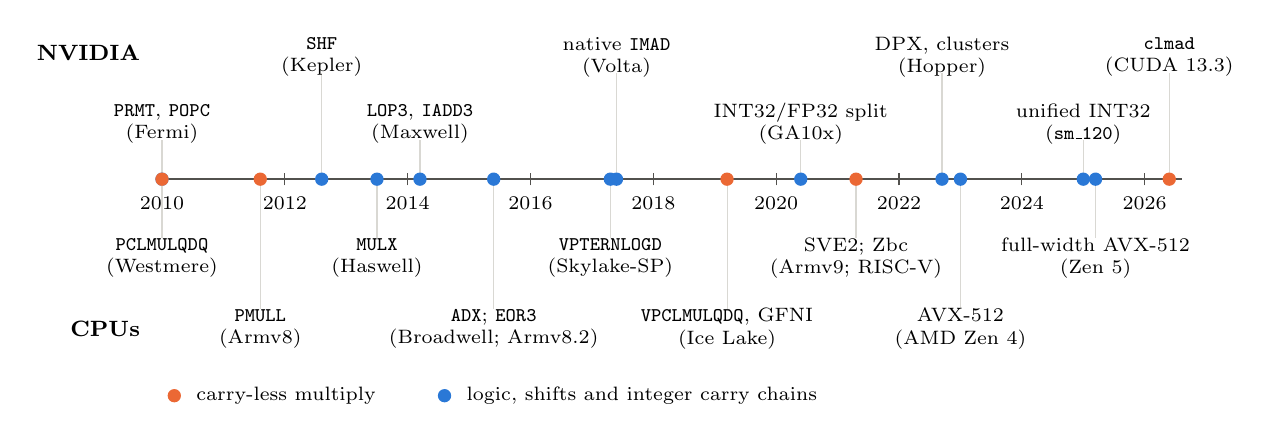
\begin{tikzpicture}[x=0.78cm,y=1cm,font=\scriptsize,
  ev/.style={circle,inner sep=1.7pt},
  lbl/.style={align=center,font=\scriptsize}]
% axis
\draw[inkS,thick] (0,0) -- (16.6,0);
\foreach \y in {0,2,...,16}{
  \draw[inkS] (\y,-0.08) -- (\y,0.08);
  \node[below,font=\scriptsize] at (\y,-0.1) {\the\numexpr2010+\y\relax};
}
\node[anchor=east,font=\footnotesize\bfseries] at (-0.2,1.6) {NVIDIA};
\node[anchor=east,font=\footnotesize\bfseries] at (-0.2,-1.9) {CPUs};
% GPU events (above)
\foreach \x/\h/\t/\c in {
  0/0.7/{\texttt{PRMT}, \texttt{POPC}\\(Fermi)}/cA,
  2.6/1.55/{\texttt{SHF}\\(Kepler)}/cA,
  4.2/0.7/{\texttt{LOP3}, \texttt{IADD3}\\(Maxwell)}/cA,
  7.4/1.55/{native \texttt{IMAD}\\(Volta)}/cA,
  10.4/0.7/{INT32/FP32 split\\(GA10x)}/cA,
  12.7/1.55/{DPX, clusters\\(Hopper)}/cA,
  15/0.7/{unified INT32\\(\texttt{sm\_120})}/cA,
  16.4/1.55/{\texttt{clmad}\\(CUDA 13.3)}/cB}{
  \draw[gridc] (\x,0) -- (\x,\h-0.2);
  \node[ev,fill=\c] at (\x,0) {};
  \node[lbl] at (\x,\h) {\t};
}
% CPU events (below)
\foreach \x/\h/\t/\c in {
  0/-1.0/{\texttt{PCLMULQDQ}\\(Westmere)}/cB,
  1.6/-1.9/{\texttt{PMULL}\\(Armv8)}/cB,
  3.5/-1.0/{\texttt{MULX}\\(Haswell)}/cA,
  5.4/-1.9/{\texttt{ADX}; \texttt{EOR3}\\(Broadwell; Armv8.2)}/cA,
  7.3/-1.0/{\texttt{VPTERNLOGD}\\(Skylake-SP)}/cA,
  9.2/-1.9/{\texttt{VPCLMULQDQ}, GFNI\\(Ice Lake)}/cB,
  11.3/-1.0/{SVE2; Zbc\\(Armv9; RISC-V)}/cB,
  13.0/-1.9/{AVX-512\\(AMD Zen 4)}/cA,
  15.2/-1.0/{full-width AVX-512\\(Zen 5)}/cA}{
  \draw[gridc] (\x,0) -- (\x,\h+0.25);
  \node[ev,fill=\c] at (\x,0) {};
  \node[lbl] at (\x,\h) {\t};
}
\node[ev,fill=cB] at (0.2,-2.75) {}; \node[anchor=west] at (0.4,-2.75) {carry-less multiply};
\node[ev,fill=cA] at (4.6,-2.75) {}; \node[anchor=west] at (4.8,-2.75) {logic, shifts and integer carry chains};
\end{tikzpicture}
\caption{When the instructions this arithmetic relies on arrived. Dates
  are first availability in a shipping product (Armv8 and Armv8.2 are
  architecture versions; Zbc is the ratification date). The GPU
  carry-less multiply arrived last of all, in 2026, which is why the
  ECC2K-130 GPU client is new work rather than a port.}
\label{fig:isa}
\end{figure}


\section{Carry-less multiply on NVIDIA GPUs}
\label{sec:blackwell}

The 2009 GPU client ran on hardware with no carry-less multiplier at
all: a binary-field product had to be assembled from AND and XOR, one
bit-slice at a time. Three things are different on current NVIDIA
parts, and between them they explain most of the gap between the
rates in Section~\ref{sec:history} and the ones in this paper.

\subsection{\texttt{clmad}}
\label{sec:blackwell-clmad}

PTX ISA~9.3, shipped with CUDA~13.3, added a carry-less multiply-add,
\texttt{clmad.lo.u64} and \texttt{clmad.hi.u64}, which returns the low
and high halves of a $64\times64$-bit product over $\FF_2$. NVIDIA
documents it for \texttt{sm\_80} and later, so it covers Ampere, Ada,
Hopper and Blackwell but not Turing~\evcite{\evref{clmad}}.
Our client uses both halves with zero addends and feeds them into a
three-leaf Karatsuba, so a $131$-bit product is six \texttt{CLMAD}
instructions. The native binary for \texttt{sm\_120} contains real
\texttt{CLMAD} opcodes in its SASS, and the build refuses to compile
the native path with anything older than CUDA~13.3 while keeping the
software product for \texttt{sm\_75} slices of a mixed
binary~\evcite{\evref{packedsrc}; \evref{ecc2k95clmad}}.

The gain depends on the part. On the RTX~PRO~6000 the native product
lifted the packed walk by $22.4\%$ ($7.110$ to $8.704$~billion
iterations/s) and roughly halved the instructions issued per update,
which is what later let the batch drop to 16 walks per inversion
(Section~\ref{sec:ledger})~\evcite{\evref{clmad}}. On Ada
the effect is larger, because the software product it replaces is
more expensive there: $1.81\times$ on the L40S and $1.88\times$ on the
L4~\evcite{\evref{ada}, §3}. On the ECC2K-95 kernel the same
port gave $1.19\times$ on the walk. The T4, at \texttt{sm\_75}, has no
\texttt{clmad} and runs the software product, which is why it sits at
the bottom of every table in this paper~\evcite{\evref{t4}}.

\subsection{\texttt{clmad} throughput}
\label{sec:blackwell-rates}

Having the instruction is not the same as having it fast. We measured
issue rates with one probe on three parts in one session
(Table~\ref{tab:clmad-dies})~\evcite{\evref{twochains}, §6.1}.

\begin{table}[t]
\centering
\small
\caption{Issue rates in lanes per SM-clock, one probe, three parts, one
  session (best of three runs per stream). The last column prices one
  \texttt{CLMAD.lo} in \texttt{LOP3} slots, which is what decides
  whether moving work onto the carry-less unit pays.}
\label{tab:clmad-dies}
\begin{tabular}{@{}lrrrrrr@{}}
\toprule
GPU & \texttt{LOP3} & \texttt{CLMAD.lo} & \texttt{CLMAD} lo+hi & \texttt{IMAD.WIDE} & \texttt{POPC} & \texttt{LOP3}/\texttt{CLMAD.lo} \\
\midrule
RTX PRO 6000 (\texttt{sm\_120}) & 63.9 & 1.69 & 1.99 & 31.3 & 16.1 & 37.8 \\
B200 (\texttt{sm\_100}) & 63.7 & 16.9 & 29.1 & 22.9 & 16.0 & 3.78 \\
H100 (\texttt{sm\_90}) & 59.8 & 29.9 & 30.1 & 22.6 & 16.0 & 2.00 \\
\bottomrule
\end{tabular}
\end{table}

The logic pipe, \texttt{POPC} and shared-memory loads run at the same
per-clock rate on all three. The carry-less unit does not. Nsight
attributes \texttt{CLMAD} to the FP64 pipe, and the workstation
Blackwell die executes FP64 at $1/64$ of its FP32 rate, about two lanes
per SM-clock; the data-centre dies run it ten to eighteen times faster
per clock. On the RTX~PRO~6000 one \texttt{CLMAD.lo} costs as much issue
time as $37.8$ logic instructions, on the B200 $3.78$, on the H100
$2.00$~\evcite{\evref{twochains}, §6}. The RTX~PRO~4500 matches the
6000 to within $1\%$~\evcite{\evref{iterfn}, §3.1 and §4.5}.

This one number reshapes the optimisation problem. On the workstation
die the carry-less unit is scarce, so the right move is to keep
products on it and everything else off it. On the data-centre dies it
is plentiful and the logic pipe binds, so the right move is the
opposite: push reductions, corrections and even basis changes onto
\texttt{CLMAD}. The same source change can therefore win on one
Blackwell part and lose on another. Moving the top-bit correction onto
\texttt{CLMAD} costs $15\%$ on the RTX~PRO~6000 and gains $13.4\%$ on the
B200; a three-limb Karatsuba loses $30\%$ on the 6000 and gains $4.9\%$
on the B200~\evcite{\evref{topclmad}; \evref{autosweep}, §3.2 and §4}.
Kernel tuning does not travel between dies, and each part in this
paper was tuned on its own.

\subsection{Integer pipe}
\label{sec:blackwell-logic}

The other instructions that matter are older but just as important.
\texttt{LOP3} evaluates any three-input Boolean function in one
instruction, which is worth $1.65\times$ on the bitsliced product
(Section~\ref{sec:arith-bitsliced}) and makes a full adder two
instructions~\evcite{\evref{client}, ``Findings''}. On the RTX~PRO~6000,
\texttt{LOP3}, \texttt{IADD3}, the funnel shift \texttt{SHF},
\texttt{PRMT} and \texttt{IMAD} all issue at about 62--63 lanes per
SM-clock, while \texttt{POPC} and \texttt{FLO} run at quarter rate
($15.8$), so each Hamming weight costs about four logic slots; the
static cost model prices them that way~\evcite{\evref{ceiling}; \evref{iterfn}, §3.1}.
The prime-field walk of Section~\ref{sec:nist} depends instead on the
carry-chain forms \texttt{mad.lo.cc}, \texttt{madc.hi.cc} and
\texttt{addc}, which exist only at 32-bit granularity; writing them by
hand was worth $1.19$--$1.38\times$ there.

Finally, the integer pipe itself got wider. Blackwell's SM lanes are
unified FP32/INT32, where Ada splits them into an FP32-only half and an
FP32/INT32 half, so the note predicted that an Ada SM would retire
integer logic at half the per-clock rate of \texttt{sm\_120}. The L40S
fits that prediction: with the software product it reached $34.4$
million iterations per second per SM, $0.427$ of the RTX~PRO~6000's
$80.4$ on its shipping build, and \texttt{CLMAD} took it to $62.2$
($0.774$)~\evcite{\evref{ada}}.
Because the walk is bound by integer logic and the carry-less unit, not
by memory bandwidth or tensor cores, the part that wins is the one with
the most SMs at the highest clock for the money, which on today's
price lists is the RTX~PRO~6000 rather than the B200
(Section~\ref{sec:survey}).

\section{GPU}
\label{sec:gpu}

On the GPU the exponent is fixed, so the only question is throughput.
As everywhere in this paper, rates are in billions of iterations per
second on one card. An iteration is one complete update of one walk,
including its share of the batched inversion, the distinguished-point
test and the restart path. Every
row here is engineering: the walk and its collision structure stay the
same, and the ratio to the generic-group floor does not move. What
does move is the ratio to a second boundary, the GPU's carry-less
unit, which we derived in Section~\ref{sec:floor} before tuning the
kernel toward it.

\begin{figure}[t]
\centering
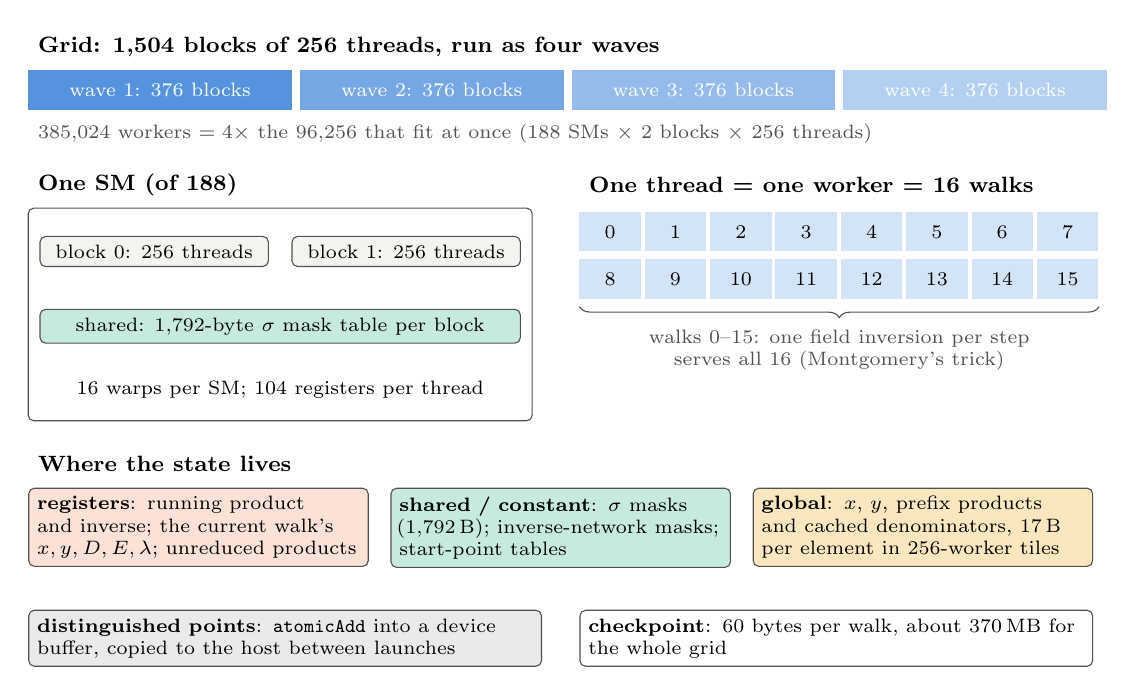
\begin{tikzpicture}[
  font=\scriptsize,x=1cm,y=1cm,
  box/.style={draw=inkS,rounded corners=2pt,fill=boxfill,align=center,inner sep=3pt},
  hdr/.style={font=\footnotesize\bfseries,anchor=west},
  arr/.style={-{Stealth[length=4pt]},inkS},
]
% ---- Row 1: grid and waves
\node[hdr] at (0,7.3) {Grid: 1{,}504 blocks of 256 threads, run as four waves};
\foreach \w in {0,1,2,3}{
  \fill[cA!\the\numexpr 80-\w*15\relax] ({\w*3.45},6.5) rectangle ({\w*3.45+3.35},7.0);
  \node[text=white] at ({\w*3.45+1.675},6.75) {wave \the\numexpr\w+1\relax: 376 blocks};
}
\node[anchor=west,text=inkS] at (0,6.2) {385{,}024 workers $=4\times$ the 96{,}256 that fit at once (188 SMs $\times$ 2 blocks $\times$ 256 threads)};
% ---- Row 2 left: one SM
\node[hdr] at (0,5.55) {One SM (of 188)};
\draw[inkS,rounded corners=2pt] (0,2.55) rectangle (6.4,5.25);
\node[box,minimum width=2.9cm] at (1.6,4.7) {block 0: 256 threads};
\node[box,minimum width=2.9cm] at (4.8,4.7) {block 1: 256 threads};
\node[box,fill=cC!25,minimum width=6.1cm] at (3.2,3.75) {shared: 1{,}792-byte $\sigma$ mask table per block};
\node at (3.2,2.95) {16 warps per SM; 104 registers per thread};
% ---- Row 2 right: one thread
\node[hdr] at (7.0,5.55) {One thread = one worker = 16 walks};
\foreach \s in {0,...,15}{
  \pgfmathsetmacro{\xx}{7.0+mod(\s,8)*0.83}
  \pgfmathsetmacro{\yy}{4.7-int(\s/8)*0.6}
  \fill[cA!20] (\xx,\yy) rectangle ({\xx+0.78},{\yy+0.5});
  \node[font=\scriptsize] at ({\xx+0.39},{\yy+0.25}) {\s};
}
\draw[decorate,decoration={brace,amplitude=4pt,mirror},inkS] (7.0,4.0) -- (13.6,4.0)
  node[midway,below=5pt,align=center] {walks 0--15: one field inversion per step\\serves all 16 (Montgomery's trick)};
% ---- Row 3: memory
\node[hdr] at (0,2.0) {Where the state lives};
\node[box,fill=cB!20,text width=4.1cm,anchor=north west,align=left] at (0,1.7)
  {\textbf{registers}: running product and inverse; the current walk's $x,y,D,E,\lambda$; unreduced products};
\node[box,fill=cC!25,text width=4.1cm,anchor=north west,align=left] at (4.6,1.7)
  {\textbf{shared / constant}: $\sigma$ masks (1{,}792\,B); inverse-network masks; start-point tables};
\node[box,fill=cD!25,text width=4.1cm,anchor=north west,align=left] at (9.2,1.7)
  {\textbf{global}: $x$, $y$, prefix products and cached denominators, 17\,B per element in 256-worker tiles};
\node[box,fill=inkS!12,text width=6.3cm,anchor=north west,align=left] at (0,0.15)
  {\textbf{distinguished points}: \texttt{atomicAdd} into a device buffer, copied to the host between launches};
\node[box,fill=white,text width=6.3cm,anchor=north west,align=left] at (7.0,0.15)
  {\textbf{checkpoint}: 60 bytes per walk, about 370\,MB for the whole grid};
\end{tikzpicture}
\caption{Anatomy of the audited $\sigma$-walk kernel on the RTX~PRO~6000.
  Each thread owns 16 walks that share one field inversion per step;
  two 256-thread blocks fit per SM, and the 385{,}024-worker grid runs in
  four waves. The 1{,}024-step loop runs inside the kernel; every step
  streams each walk's compact state through global memory, and the
  distinguished-point buffer is drained between launches.}
\label{fig:kernel}
\end{figure}


\begin{figure}[t]
\centering
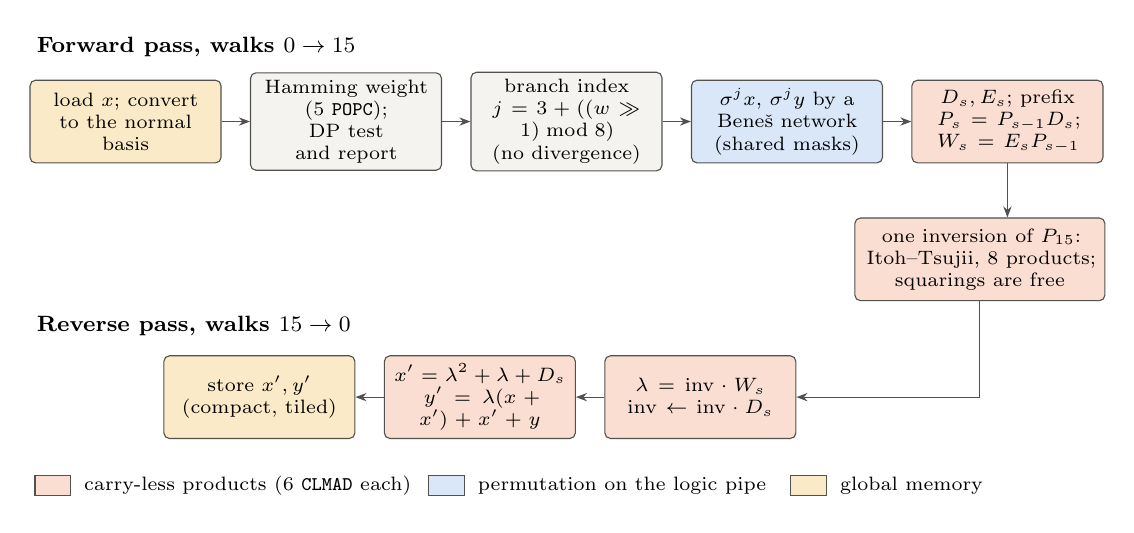
\begin{tikzpicture}[
  font=\scriptsize,x=1cm,y=1cm,
  st/.style={draw=inkS,rounded corners=2pt,fill=boxfill,align=center,inner sep=2.5pt,minimum height=1.05cm,text width=2.25cm},
  clm/.style={st,fill=cB!22},
  net/.style={st,fill=cA!18},
  mem/.style={st,fill=cD!22},
  arr/.style={-{Stealth[length=4pt]},inkS},
  lane/.style={font=\footnotesize\bfseries,anchor=west},
]
% Forward pass
\node[lane] at (-0.1,0.95) {Forward pass, walks $0\to15$};
\node[mem] (f1) at (1.15,0) {load $x$; convert\\to the normal\\basis};
\node[st]  (f2) at (3.95,0) {Hamming weight\\(5 \texttt{POPC});\\DP test and report};
\node[st]  (f3) at (6.75,0) {branch index\\$j=3+((w\gg1)\bmod8)$\\(no divergence)};
\node[net] (f4) at (9.55,0) {$\sigma^j x$, $\sigma^j y$ by a\\Bene\v{s} network\\(shared masks)};
\node[clm] (f5) at (12.35,0) {$D_s,E_s$; prefix\\$P_s=P_{s-1}D_s$;\\$W_s=E_sP_{s-1}$};
\foreach \a/\b in {f1/f2,f2/f3,f3/f4,f4/f5} \draw[arr] (\a)--(\b);
% Inversion
\node[clm,text width=3.0cm] (inv) at (12.0,-1.75) {one inversion of $P_{15}$:\\Itoh--Tsujii, 8 products;\\squarings are free};
\draw[arr] (f5) -- (f5|-inv.north);
% Reverse pass
\node[lane] at (-0.1,-2.6) {Reverse pass, walks $15\to0$};
\node[clm] (r1) at (8.45,-3.5) {$\lambda=\mathrm{inv}\cdot W_s$\\$\mathrm{inv}\leftarrow\mathrm{inv}\cdot D_s$};
\node[clm] (r2) at (5.65,-3.5) {$x'=\lambda^2+\lambda+D_s$\\$y'=\lambda(x+x')+x'+y$};
\node[mem] (r3) at (2.85,-3.5) {store $x',y'$\\(compact, tiled)};
\draw[arr] (inv.south) |- (r1.east);
\draw[arr] (r1)--(r2); \draw[arr] (r2)--(r3);
% Key
\begin{scope}[shift={(0,-4.75)}]
\fill[cB!22,draw=inkS] (0,0) rectangle (0.45,0.25); \node[anchor=west] at (0.5,0.125) {carry-less products (6 \texttt{CLMAD} each)};
\fill[cA!18,draw=inkS] (5.0,0) rectangle (5.45,0.25); \node[anchor=west] at (5.5,0.125) {permutation on the logic pipe};
\fill[cD!22,draw=inkS] (9.6,0) rectangle (10.05,0.25); \node[anchor=west] at (10.1,0.125) {global memory};
\end{scope}
\end{tikzpicture}
\caption{One step of the $\sigma$-walk for the 16 walks of a thread. The
  forward pass computes each walk's denominator and a running prefix
  product; one inversion of the final product then serves all 16; the
  reverse pass peels off each walk's inverse and finishes the affine
  addition. Per walk that is $4.81$ products of six \texttt{CLMAD} each plus
  a sixteenth of the inversion; everything else, including every
  Frobenius power, runs on the logic pipe.}
\label{fig:step}
\end{figure}


\subsection{Floor and roofline}
\label{sec:floor}

Any walk that keeps the rho collision structure performs one affine
addition per iteration. With Montgomery's batched
inversion~\cite{montgomery1987} across $W$ walks, that addition costs
a fixed number of field products plus $1/W$ of an inversion. In the
packed representation a $131\times131$ product is a two-way Karatsuba
over $64\times64$ carry-less multiplies, which is six \texttt{CLMAD}
instructions. At batch $W=16$ the shipping kernel issues 77 products
per 16 slots, or $4.81$ per update. Table~\ref{tab:floor} prices one
update on the RTX~PRO~6000 (188 SMs)~\evcite{\evref{iterfn}, §1}.

\begin{table}[t]
\centering
\small
\caption{Arithmetic floor of one affine-addition update on the
  RTX~PRO~6000, and the budgets three throughput targets allow at
  $100\%$ pipe utilisation. The carry-less unit issues $1.65$ lane operations per SM-clock
  ($1/37.7$ of the logic pipe's $62.1$, measured on an RTX~PRO~4500 with
  the same SM and later confirmed on the 6000 at $1/38.0$); sustained
  clock $2.30$~GHz, maximum $2.43$~GHz. Both floors sit
  above the $28$~billion iterations/s budget.}
\label{tab:floor}
\begin{tabular}{@{}lrr@{}}
\toprule
component & \texttt{CLMAD}/upd. & ALU slots/upd. \\
\midrule
$4.81$ products ($6$ \texttt{CLMAD} each) & $28.9$ & $\approx 830$ \\
squarings & $5.0$ & $\approx 80$ \\
batched inversion ($/16$) & $4.6$ & $\approx 270$ \\
\midrule
floor & $38.5$ ($28.9$, squarings on ALU) & $1{,}090$--$1{,}180$ \\
\midrule
budget at $14.64$~billion iterations/s & $48.7$--$51.4$ & $1{,}834$--$1{,}938$ \\
budget at $20$~billion iterations/s & $35.6$--$37.6$ & $1{,}343$--$1{,}418$ \\
budget at $28$~billion iterations/s & $25.4$--$26.9$ & $959$--$1{,}013$ \\
\bottomrule
\end{tabular}
\end{table}

The two pipes are independent, and each sets its own floor. On the
carry-less unit, $28.9$ \texttt{CLMAD} at $1.65$ lanes per SM-clock is
$17.5$ SM-clocks per update, a ceiling of $24.7$--$26.1$~billion iterations/s even if
everything else were free. On the logic pipe, about $1{,}090$ ALU slots
already exceed the $959$--$1{,}013$ that $28$~billion iterations/s would allow. At $90\%$
utilisation of either pipe the ceiling is $22.2$--$23.4$~billion iterations/s. The note
was written to decide whether a different iteration function could
take one card from the audited $14.64$ to $28$~billion iterations/s. The
answer came before any kernel was built: it cannot, because $28$~billion iterations/s
is below the floor of any walk that performs one affine addition per
iteration.

Our estimate of the carry-less rate went up as the kernels got closer
to it. A kernel-mix measurement on the 6000 at $1.62$
lane-\texttt{CLMAD}s per SM-clock priced the $20$~billion iterations/s table-walk kernel
at $33.1$ \texttt{CLMAD} per update ($28.9$ products, $3.0$ inversion,
$1.25$ normal-basis squarings) and gave a floor of
$22.3$~billion iterations/s~\evcite{\evref{twochains}, §1}. A screened (not yet
verified) three-limb Karatsuba arm then implied at least $1.654$
lane-\texttt{CLMAD}s per SM-clock, which refuted that figure. The
roofline of the $20.078$~billion iterations/s build (Table~\ref{tab:roofline}) puts the
carry-less speed of light at $27.4$~billion iterations/s with the unit $2.00$ lanes
wide, while the logic pipe, at $1{,}319.6$ lane-instructions per
update, is $91.2\%$ busy and runs out first~\evcite{\evref{roofline}}.
Thirty billion iterations/s would need at most $30.3$ \texttt{CLMAD} and $968$ ALU slots
per update, a $27\%$ cut in integer work that the note calls ``a
two-card number''. The $28$~billion iterations/s verdict survives the revision because
it never rested on the carry-less unit alone.

\begin{table}[t]
\centering
\small
\caption{Roofline of the $20.078$~billion iterations/s table-walk build on the
  RTX~PRO~6000: 188 SMs at $2.415$~GHz, $22.61$ SM-clocks per update.
  Work per update is lane-instructions from the dynamic count (Section~\ref{sec:profiling}); the ceiling is the
  rate at which that unit alone would saturate.}
\label{tab:roofline}
\begin{tabular}{@{}lrrrr@{}}
\toprule
unit & peak lanes/SM-clk & work/update & ceiling (billion it/s) & busy \\
\midrule
ALU (logic) & 64 & $1{,}319.6$ & $22.0$ & $91.2\%$ \\
\texttt{CLMAD} & $2.00$ & $33.1$ & $27.4$ & $73.2\%$ \\
issue & 128 & $1{,}698.9$ & $34.2$ & $58.7\%$ \\
load/store & 16 & $80.0$ & $90.8$ & $22.1\%$ \\
FMA & 64 & $188.6$ & $154$ & $13.0\%$ \\
\bottomrule
\end{tabular}
\end{table}

\begin{figure}[t]
\centering
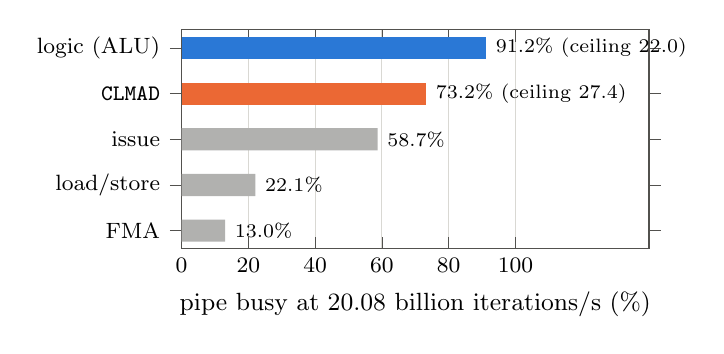
\begin{tikzpicture}
\begin{axis}[
  xbar, bar width=8pt, bar shift=0pt,
  width=0.62\textwidth, height=0.36\textwidth,
  xmin=0, xmax=140, xtick={0,20,...,100},
  xlabel={pipe busy at 20.08 billion iterations/s (\%)},
  symbolic y coords={alu,clmad,issue,lsu,fma},
  ytick={alu,clmad,issue,lsu,fma},
  yticklabels={logic (ALU),\texttt{CLMAD},issue,load/store,FMA},
  y dir=reverse, xmajorgrids,
  nodes near coords, nodes near coords style={font=\scriptsize,anchor=west},
  point meta=explicit symbolic,
]
\addplot[fill=cA,draw=none] coordinates {(91.2,alu) [91.2\% (ceiling 22.0)]};
\addplot[fill=cB,draw=none] coordinates {(73.2,clmad) [73.2\% (ceiling 27.4)]};
\addplot[fill=inkS!45,draw=none] coordinates {(58.7,issue) [58.7\%] (22.1,lsu) [22.1\%] (13.0,fma) [13.0\%]};
\end{axis}
\end{tikzpicture}
\caption{The roofline of Table~\ref{tab:roofline} as a picture: the logic
  pipe is the binding constraint for the table walk's arithmetic on the
  RTX~PRO~6000, with the carry-less unit second; memory and the FMA pipe
  are far from busy. In brackets, the rate at which each unit alone would
  saturate, in billions of iterations per second. Utilisation comes from
  dynamic instruction counts and measured pipe rates, not hardware
  counters (Section~\ref{sec:profiling}).}
\label{fig:roofline}
\end{figure}


The same note measures the carry-less unit on other dies: $37.8$
logic slots per \texttt{CLMAD.lo} on the 6000, $3.78$ on the B200 and
$2.00$ on the H100. On the data-centre parts, then, the logic pipe
binds by a wide margin, and on the B200 the carry-less floor alone
would be $255$~billion iterations/s~\evcite{\evref{twochains}, §6.1--6.2}.

We had to correct the static accounting behind Table~\ref{tab:floor}
once. An earlier SASS counter reported about $1{,}570$ ALU slots and
$29$ \texttt{CLMAD} per update; its replacement counts $2{,}271$ ALU and
$45$ \texttt{CLMAD} statically, or $2{,}324$ once \texttt{POPC} and
\texttt{FLO} are priced at their measured quarter
rate~\evcite{\evref{iterfn}, §3}. The floor argument does
not depend on which count is used, since the budgets are below both.

\subsection{Acceptance criteria}
\label{sec:gates}

With two exceptions named in Section~\ref{sec:declined}, every step
in this section is a paired comparison on one GPU allocation: the
candidate and control are interleaved, three to six repetitions each,
and we report the candidate's ratio to the control for every pair. We
adopt a change only if it clears a rule declared before the run. For
most of the ledger that rule is a gain of at least $1\%$ on both the
benchmark and the DP34 collection workload, with every pair favouring
the candidate. For the later table-walk work it is a geometric-mean
ratio at or above a stated threshold, with every pair above a stated
minimum~\evcite{\evref{nativecand}; \evref{sigmatable}}.
Every adopted kernel re-walks every device report on the host
reference ($300$ of $300$ in the later notes) and recovers planted
logarithms on $\mathrm{GF}(2^{41})$. A candidate that fails the rule
stays in the tree behind a flag, with its ratio on record;
Section~\ref{sec:declined} collects them.

\subsection{Profiling}
\label{sec:profiling}

Each number in this section comes from one of five instruments, and
we say which.

\paragraph{Rates.} A rate is the client's own count of complete scalar
updates divided by wall time over the timed launches, as printed at
the end of a \texttt{-{}-bench} run. Distinguished-point reporting is off
in the timed invocation; a separate run of the same binary re-walks its
device reports on the host reference. Candidates and controls are
timed in interleaved pairs on one allocation (Section~\ref{sec:gates}).
Where a rate is converted to SM-clocks per update, the SM clock is the
median sampled with \texttt{nvidia-smi} after the timed
runs~\evcite{\evref{roofline}, §2}.

\paragraph{Static instruction counts.} A script compiles the walk kernel
with the preset's exact flags, disassembles the SASS with
\texttt{cuobjdump}, finds the step and slot loops from their backward
branches, weights each loop body by its trip count and charges every
out-of-line callee to its call sites. It reports logic, integer-multiply,
\texttt{CLMAD} and memory lane-instructions per update, with registers,
spills and stack frame from \texttt{ptxas -v}. Because a static count
includes both arms of every predicated branch, it is an upper bound on
what a warp issues~\evcite{\evref{iterfn}, §3; \evref{probes}}.

\paragraph{Dynamic instruction counts.} For the roofline
(Table~\ref{tab:roofline}) a second tool disassembles with
\texttt{nvdisasm}, builds the control-flow graph, gives each branch a
probability from the source (loop trip counts; rare events such as a
distinguished point near zero), solves the visit equations exactly and
prices each instruction on the pipe that executes it. Two checks bind
the result: the dynamic \texttt{CLMAD} count must equal the count the
arithmetic implies ($33.125$ per update for the $20.08$ build, and all
46 sweep builds pass), and the analysed kernel must match the full
client's SASS instruction for instruction ($4{,}920$ of $4{,}920$ for
that build)~\evcite{\evref{roofline}, §1}.

\paragraph{Pipe rates.} Microbenchmarks price each instruction class
on the device. Each stream issues one kind of instruction in sixteen
independent accumulator chains, so issue rate rather than latency is
measured, with no memory traffic and a host check on the result; the
streams alternate and repeat, so thermal drift is not charged to
whichever ran last. On the RTX~PRO~6000 they give $62$--$64$ lanes per
SM-clock for \texttt{LOP3}, \texttt{IADD3} and \texttt{SHF}, $62.3$ for
\texttt{IMAD}, about $16$ for \texttt{POPC} and shared-memory loads, and
about two for \texttt{CLMAD} in an isolated stream, somewhat less inside
the walk (Section~\ref{sec:blackwell-rates})~\evcite{\evref{probes}; \evref{roofline}, §2}.
Inside the walk, a \texttt{clock64()} phase build has lane 0 of every
warp accumulate the cycles of the forward pass, the inversion and the
reverse pass, and counter builds tally events such as cycle-probe hints,
which is how the v3 latency of Section~\ref{sec:sigma-vs-table} was
traced~\evcite{\evref{oneblock}; \evref{probelat}}.

\paragraph{Hardware counters.} Nsight Compute read counters on one
RTX~PRO~6000 host with root access, for two builds of the ledger. On
the $17.30$~billion iterations/s control it put the FP64 pipe, which
executes \texttt{CLMAD}, at $71\%$, the logic pipe at $36\%$ and DRAM at
$11\%$; on the $17.41$ build, issue at $52\%$ with $3.44$ active and
$1.04$ eligible warps per scheduler~\evcite{\evref{tp29}, §5}. It is also the source of the
attribution of \texttt{CLMAD} to the FP64 pipe
(Section~\ref{sec:blackwell-rates}). On a rented RTX~PRO~4500 every
Nsight Compute command failed before producing counters, and Modal
containers do not expose them; Nsight Systems traces from those runs
were used only to separate launch overhead ($0.113$~ms of launch calls
against $628.6$~ms of kernel time) from work inside the kernel, never as
a rate~\evcite{\evref{goal28}, ``Nsight findings''}. The pipe utilisation
of the $20.08$ build and of every later build therefore comes from the
dynamic counts and the measured pipe rates, not from hardware counters.

\subsection{Ledger}
\label{sec:ledger}

The original client was bitsliced, with 32 walks in the bit lanes of
a word and every field operation a straight-line program of
\texttt{LOP3} instructions (Section~\ref{sec:arith-bitsliced}). When
we audited the packed replacement, that control measured
$0.852294$~billion iterations/s on an RTX~PRO~6000~\evcite{\evref{packed}}.
Table~\ref{tab:ledger} traces the path from there to the audited
$14.637530$~billion iterations/s ($14.106673$~billion iterations/s while collecting at weight 34). Each
step is the corresponding note's own paired comparison. They do not
form a single chain at constant occupancy and compiler, and where a
note changed more than one thing at once, the table says so.

\begin{table}[t]
\centering
\small
\caption{Packed-backend rungs on one RTX~PRO~6000. Each gain is the
  note's own paired comparison against the adjacent control, not a
  ratio of non-adjacent headlines. Blocks/SM is the resident-block bound; ``conf.'' marks a comparison
  that also changed occupancy, compiler or walk population (the packed
  row's control ran $49$~M walks once and its candidate $1.5$~M walks
  three times). Class: engineering.}
\label{tab:ledger}
\begin{tabular}{@{}p{0.40\textwidth}rrl@{}}
\toprule
rung & control & candidate & gain \\
\midrule
bitsliced control & --- & $0.852294$ & baseline \\
packed normal basis, five words (conf.) & $0.852294$ & $2.957961$ & $3.47\times$ \\
single polynomial product, 2 blocks/SM & $2.956981$ & $3.366572$ & $+13.85\%$ \\
denominator cache, 4 blocks/SM & $3.506509$ & $4.024103$ & $+14.76\%$ \\
\quad same, 6 blocks/SM (conf.) & $3.506509$ & $4.094367$ & $+16.76\%$ \\
Frobenius permutation networks & $4.115575$ & $5.811421$ & $+41.21\%$ \\
polynomial-basis batch chain (conf.) & $5.832342$ & $6.054107$ & $+3.80\%$ \\
paired products (conf.) & $6.123614$ & $6.215430$ & $+1.50\%$ \\
polynomial-basis state & $6.301859$ & $6.547850$ & $+3.90\%$ \\
direct reduction & $6.826154$ & $6.906059$ & $+1.17\%$ \\
generated straight-line product (conf.) & $6.860749$ & $6.924275$ & $+0.93\%$ \\
256-worker tiles & $6.852888$ & $6.994745$ & $+2.07\%$ \\
native \texttt{clmad} (CUDA 13.3) & $7.110440$ & $8.703518$ & $+22.40\%$ \\
batch 16, $385{,}024$ workers & $8.673447$ & $13.206088$ & $+52.26\%$ \\
weighted prefixes, paired Frobenius & $13.110335$ & $13.323276$ & $+1.62\%$ \\
compact 17-byte state & $13.548376$ & $14.403112$ & $+6.31\%$ \\
shared-memory mask table & $14.296584$ & $14.411102$ & $+0.80\%$ \\
\quad public audit of that build & --- & $14.637530$ & DP34 $14.106673$ \\
\bottomrule
\end{tabular}
\end{table}

Sources, one per rung: packed basis~\evcite{\evref{packed}}; single
product~\evcite{\evref{singleprod}}; denominator
cache~\evcite{\evref{dencache}}; Frobenius
networks~\evcite{\evref{frobnet}}; polynomial
chain~\evcite{\evref{polychain}}; paired
products~\evcite{\evref{pairedprod}}; polynomial
state~\evcite{\evref{polystate}}; direct
reduction~\evcite{\evref{directred}}; generated
product~\evcite{\evref{genprod}}; tiles~\evcite{\evref{tiles}};
native carry-less~\evcite{\evref{clmad}}; batch
tuning~\evcite{\evref{batch}}; weighted
prefixes~\evcite{\evref{wprefix}}; compact
state~\evcite{\evref{compact}}; shared
masks~\evcite{\evref{sharedsigma}}.

\begin{figure}[t]
\centering
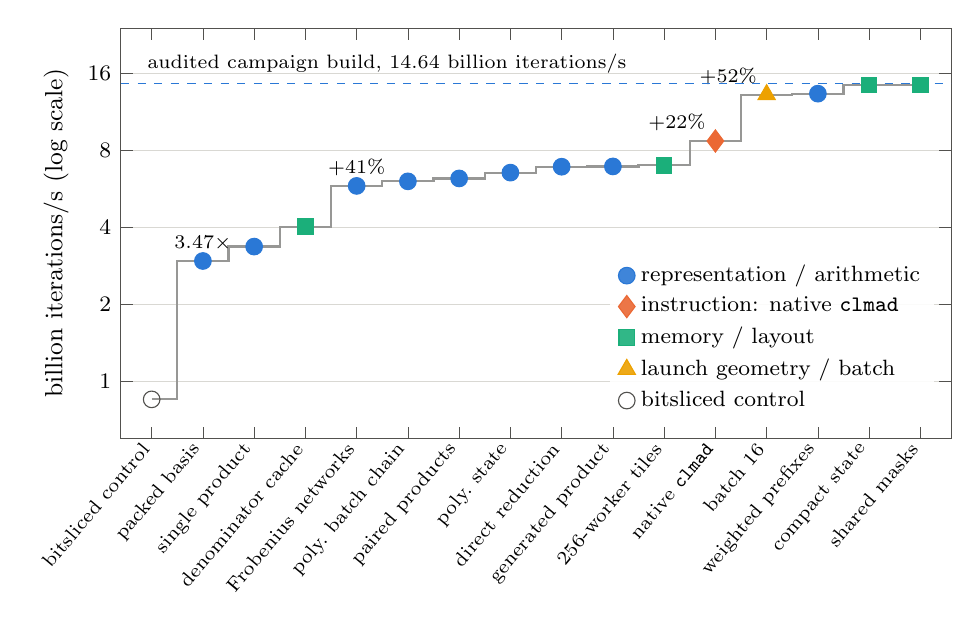
\begin{tikzpicture}
\begin{axis}[
  width=\textwidth, height=0.56\textwidth,
  ymode=log, log basis y=10,
  ymin=0.6, ymax=24,
  xmin=-0.6, xmax=15.6,
  ytick={1,2,4,8,16}, yticklabels={1,2,4,8,16},
  ylabel={billion iterations/s (log scale)},
  xtick={0,...,15},
  xticklabels={
    bitsliced control, packed basis, single product, denominator cache,
    Frobenius networks, poly.\ batch chain, paired products, poly.\ state,
    direct reduction, generated product, 256-worker tiles, native \texttt{clmad},
    batch 16, weighted prefixes, compact state, shared masks},
  x tick label style={rotate=50,anchor=east,font=\scriptsize},
  ymajorgrids,
  legend style={at={(0.98,0.04)},anchor=south east,fill=white,fill opacity=0.9,text opacity=1},
  legend cell align=left,
]
\addplot[inkS!60,thick,const plot mark mid,forget plot] coordinates {
  (0,0.852) (1,2.958) (2,3.367) (3,4.024) (4,5.811) (5,6.054) (6,6.215)
  (7,6.548) (8,6.906) (9,6.924) (10,6.995) (11,8.704) (12,13.206)
  (13,13.323) (14,14.403) (15,14.411)};
\addplot[only marks,mark=*,mark size=3pt,color=cA] coordinates {
  (1,2.958) (2,3.367) (4,5.811) (5,6.054) (6,6.215) (7,6.548) (8,6.906)
  (9,6.924) (13,13.323)};
\addlegendentry{representation / arithmetic}
\addplot[only marks,mark=diamond*,mark size=4pt,color=cB] coordinates {(11,8.704)};
\addlegendentry{instruction: native \texttt{clmad}}
\addplot[only marks,mark=square*,mark size=2.8pt,color=cC] coordinates {
  (3,4.024) (10,6.995) (14,14.403) (15,14.411)};
\addlegendentry{memory / layout}
\addplot[only marks,mark=triangle*,mark size=3.6pt,color=cD] coordinates {(12,13.206)};
\addlegendentry{launch geometry / batch}
\addplot[only marks,mark=o,mark size=3pt,color=inkS] coordinates {(0,0.852)};
\addlegendentry{bitsliced control}
\node[font=\scriptsize,anchor=south] at (axis cs:1,2.958) {$3.47\times$};
\node[font=\scriptsize,anchor=south] at (axis cs:4,5.811) {$+41\%$};
\node[font=\scriptsize,anchor=south east] at (axis cs:11,8.704) {$+22\%$};
\node[font=\scriptsize,anchor=south east] at (axis cs:12,13.206) {$+52\%$};
\draw[dashed,cA] (axis cs:-0.6,14.64) -- (axis cs:15.6,14.64)
  node[pos=0.02,anchor=south west,font=\scriptsize,color=black] {audited campaign build, 14.64 billion iterations/s};
\end{axis}
\end{tikzpicture}
\caption{The packed-backend ledger on one RTX~PRO~6000
  (Table~\ref{tab:ledger}), each step's candidate rate, with the marker
  showing what kind of change it was. No step changed the walk: the
  iteration function, the step count and the distinguished points are
  the same throughout. Steps are separate paired comparisons, not one
  chain, so the line joins candidates measured in different sessions.}
\label{fig:ledger}
\end{figure}

% Segment lengths are log10(factor) * \k cm, so widths multiply like the factors.
\begin{figure}[t]
\centering
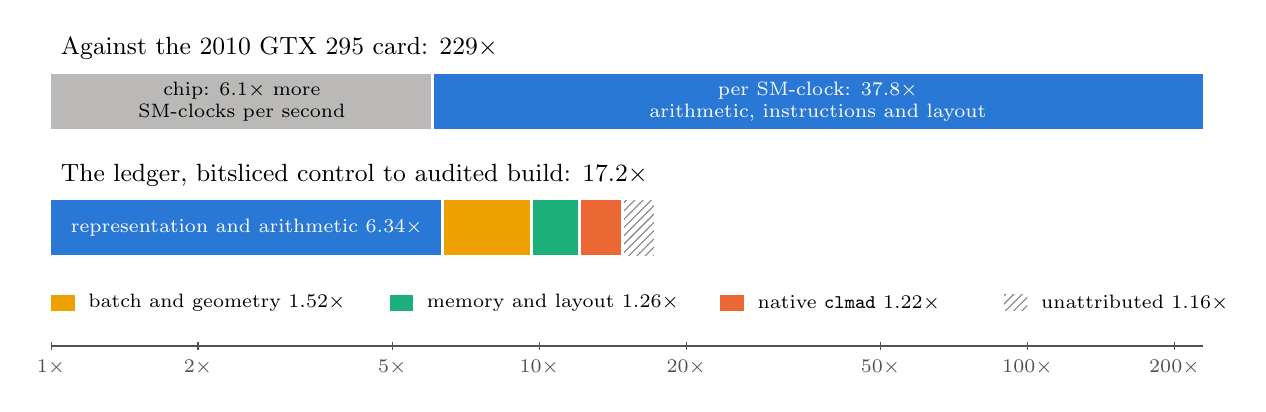
\begin{tikzpicture}[x=1cm,y=1cm,lab/.style={font=\scriptsize,align=center}]
\def\k{6.2}
% Row 1: 2010 GTX 295 -> RTX PRO 6000, 228.75x = SM-clocks 6.05x x per-SM-clock 37.8x
\pgfmathsetmacro{\p}{\k*log10(6.05)}
\pgfmathsetmacro{\q}{\k*log10(228.75)}
\node[anchor=south west,font=\small] at (0,2.62) {Against the 2010 GTX~295 card: $229\times$};
\fill[inkS!40] (0,1.85) rectangle (\p,2.55);
\fill[cA] (\p,1.85) rectangle (\q,2.55);
\draw[white,line width=1pt] (\p,1.85)--(\p,2.55);
\node[lab] at (\p/2,2.2) {chip: $6.1\times$ more\\SM-clocks per second};
\node[lab,text=white] at ({(\p+\q)/2},2.2) {per SM-clock: $37.8\times$\\arithmetic, instructions and layout};
% Row 2: ledger 0.852 -> 14.64, 17.17x
\pgfmathsetmacro{\a}{\k*log10(6.337)}
\pgfmathsetmacro{\b}{\a+\k*log10(1.523)}
\pgfmathsetmacro{\c}{\b+\k*log10(1.255)}
\pgfmathsetmacro{\d}{\c+\k*log10(1.224)}
\pgfmathsetmacro{\e}{\k*log10(17.17)}
\node[anchor=south west,font=\small] at (0,1.0) {The ledger, bitsliced control to audited build: $17.2\times$};
\fill[cA] (0,0.25) rectangle (\a,0.95);
\fill[cD] (\a,0.25) rectangle (\b,0.95);
\fill[cC] (\b,0.25) rectangle (\c,0.95);
\fill[cB] (\c,0.25) rectangle (\d,0.95);
\fill[white] (\d,0.25) rectangle (\e,0.95);
\fill[pattern=north east lines,pattern color=inkS!70] (\d,0.25) rectangle (\e,0.95);
\draw[white,line width=1pt] (\a,0.25)--(\a,0.95) (\b,0.25)--(\b,0.95) (\c,0.25)--(\c,0.95) (\d,0.25)--(\d,0.95);
\node[lab,text=white] at (\a/2,0.6) {representation and arithmetic $6.34\times$};
% Key for the narrow segments, in bar order.
\begin{scope}[shift={(0,-0.45)}]
\fill[cD] (0,0) rectangle (0.3,0.2); \node[lab,anchor=west] at (0.35,0.1) {batch and geometry $1.52\times$};
\fill[cC] (4.3,0) rectangle (4.6,0.2); \node[lab,anchor=west] at (4.65,0.1) {memory and layout $1.26\times$};
\fill[cB] (8.5,0) rectangle (8.8,0.2); \node[lab,anchor=west] at (8.85,0.1) {native \texttt{clmad} $1.22\times$};
\fill[pattern=north east lines,pattern color=inkS!70] (12.1,0) rectangle (12.4,0.2); \node[lab,anchor=west] at (12.45,0.1) {unattributed $1.16\times$};
\end{scope}
% log scale
\draw[inkS] (0,-0.9) -- (\q,-0.9);
\foreach \v in {1,2,5,10,20,50,100,200}
  \draw[inkS] ({\k*log10(\v)},-0.85) -- ({\k*log10(\v)},-0.95) node[below,font=\scriptsize] {$\v\times$};
\end{tikzpicture}
\caption{Where the speedup came from, on a log scale so that segment
  widths multiply. Top: against the 2010 GTX~295 card, about $6\times$ is a
  bigger, faster chip and about $38\times$ is per-SM-clock work. Bottom: the
  sixteen paired ledger steps grouped by kind (Figure~\ref{fig:ledger});
  their gains multiply to $14.8\times$ against the $17.2\times$ from the
  bitsliced control to the audited build, and the remaining $1.16\times$ is
  steps taken outside the ledger (launch shape, a compiler upgrade) and
  session-to-session drift. None of it changed the rho algorithm.}
\label{fig:gains}
\end{figure}


Three steps account for most of the factor, and each is a change of
representation rather than a tuning knob. The Frobenius permutation
networks ($+41\%$) replace the repeated squarings that computed
$\sigma^j$ with fixed Bene\v{s} permutation networks over the permuted
normal basis,
checked on $3{,}120$ GPU vectors and on $256$ basis vectors under all
$131$ powers. Native carry-less multiplication ($+22\%$) replaces an
emulated $32\times32$ carry-less product with the
\texttt{clmad.lo}/\texttt{hi} instructions that CUDA~13.3 exposes
(Section~\ref{sec:blackwell-clmad}). That change in turn let the batch drop from 32 to 16 walks
per inversion with $385{,}024$ workers, four times the $96{,}256$ that
fit on the card at once, so the grid runs in four waves ($+52\%$), at the
same two-block occupancy and the same 122 registers per thread. The note
suggests a cache-capacity explanation (the hot state shrinks from $245$
to $122$~MiB) but did not measure it~\evcite{\evref{batch}}.
Between the Frobenius-network confirmation ($5.81$~billion iterations/s) and the
shipping walk ($14.64$~billion iterations/s), the gain is those two changes plus layout
work. The table gives each its own pair, and we do not quote any single
``remaining factor'' as if it had been measured.

The $\sigma$-walk did not stop at $14.64$. A fused single-pass variant
measured $15.436677$ against $15.015004$~billion iterations/s ($1.028\times$, five
pairs). A $\sigma$ step through nibble tables in shared memory
($68{,}352$ bytes, $512\times1$ blocks) measured $15.884369$ against
$15.513653$~billion iterations/s, a paired median of $1.023930$ with every pair at or
above $1.0238$ and an A/A drift of $0.099\%$. That clears a
pre-registered gate of geometric mean $\ge1.015$ with every pair
$\ge1.005$~\evcite{\evref{sigmafused}; \evref{sigmatable}}.
A later screen of the same nibble-table build on two rented RTX~PRO~6000
cards measured $15.99$ and $15.76$~billion iterations/s, $31.75$ together,
with 300 of 300 reports re-walked on each; it is an unpaired screen,
not a paired panel~\evcite{\evref{redesign}}.
These are the current $\sigma$-walk headlines. The campaign
configuration of Section~\ref{sec:campaign} was frozen before they
existed and still ships the audited $14.64$ build.

\subsection{Speedup breakdown}
\label{sec:what-changed}

None of the sixteen steps changed the algorithm. The iteration function
$R\mapsto\sigma^j(R)+R$, the branch rule, the distinguished-point rule,
the seeds and therefore the expected number of iterations are those of
Bailey et al.\ at every step; from the direct reduction onward each
adopted build produced the byte-identical sorted corpus of $5{,}149$
distinguished points on the same workload, and the earlier steps matched
their controls' checkpoints byte for byte~\evcite{\evref{compact}; \evref{sharedsigma}}.
What changed is how a step is computed, and Figure~\ref{fig:gains} splits
that by kind. Representation and arithmetic (the packed basis, one
product instead of two, the Frobenius networks, the polynomial-basis
state and its reduction) account for $6.3\times$; launch geometry and
batch size for $1.5\times$; memory layout (the denominator cache, tiles,
compact state and shared masks) for $1.3\times$; and the one new hardware
feature, \texttt{clmad}, for $1.2\times$ directly, plus the batch change it
enabled. Figures~\ref{fig:kernel} through~\ref{fig:tiling} show the
resulting kernel. The changes that do alter the walk, the table walk and
the RTX~PRO~4500's bridge map, are kept separate and labelled as
iteration-function changes, because they change the walk constant as
well as the rate (Section~\ref{sec:walk-cycles}).

\begin{figure}[t]
\centering
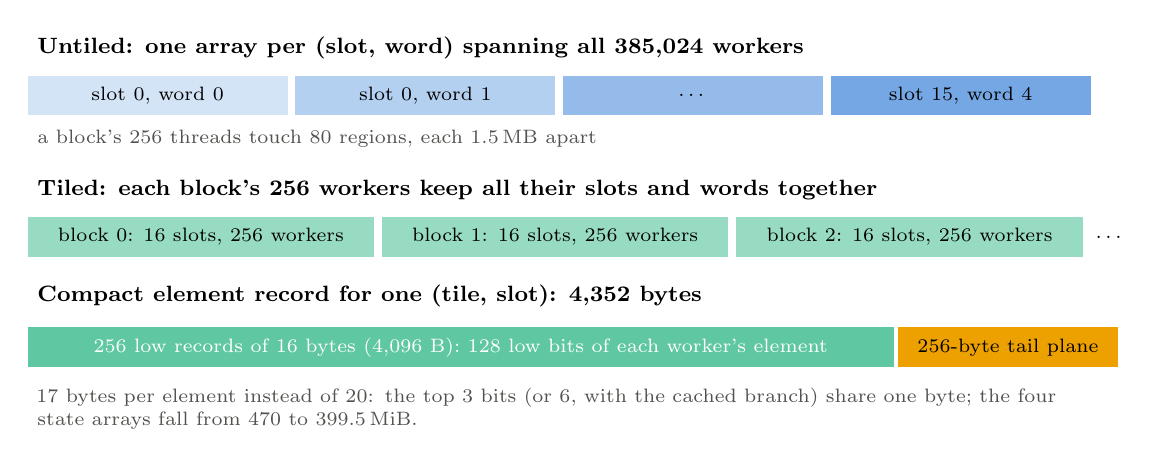
\begin{tikzpicture}[font=\scriptsize,x=1cm,y=1cm]
% Untiled
\node[anchor=west,font=\footnotesize\bfseries] at (0,3.45) {Untiled: one array per (slot, word) spanning all 385{,}024 workers};
\foreach \i/\t in {0/{slot 0, word 0},1/{slot 0, word 1},2/{\dots},3/{slot 15, word 4}}{
  \fill[cA!\the\numexpr 20+\i*15\relax] ({\i*3.4},2.6) rectangle ({\i*3.4+3.3},3.1);
  \node at ({\i*3.4+1.65},2.85) {\t};
}
\node[anchor=west,text=inkS] at (0,2.3) {a block's 256 threads touch 80 regions, each 1.5\,MB apart};
% Tiled
\node[anchor=west,font=\footnotesize\bfseries] at (0,1.65) {Tiled: each block's 256 workers keep all their slots and words together};
\foreach \b in {0,1,2}{
  \fill[cC!45] ({\b*4.5},0.8) rectangle ({\b*4.5+4.4},1.3);
  \node at ({\b*4.5+2.2},1.05) {block \b: 16 slots, 256 workers};
}
\node at (13.75,1.05) {\dots};
% Compact record
\node[anchor=west,font=\footnotesize\bfseries] at (0,0.3) {Compact element record for one (tile, slot): 4{,}352 bytes};
\fill[cC!70] (0,-0.6) rectangle (11.0,-0.1);
\node[text=white] at (5.5,-0.35) {256 low records of 16 bytes (4{,}096 B): 128 low bits of each worker's element};
\fill[cD] (11.05,-0.6) rectangle (13.85,-0.1);
\node at (12.45,-0.35) {256-byte tail plane};
\node[anchor=north west,text=inkS,align=left,text width=13.6cm] at (0,-0.75)
  {17 bytes per element instead of 20: the top 3 bits (or 6, with the cached branch) share one byte;
   the four state arrays fall from 470 to 399.5\,MiB.};
\end{tikzpicture}
\caption{How walk state is laid out in global memory. Tiling puts all of
  a block's state in one contiguous region while each warp still reads
  adjacent words ($+2.1\%$); the compact record then packs each 131-bit
  element into 17 bytes ($+6.3\%$). Neither changes a single bit of the
  walk.}
\label{fig:tiling}
\end{figure}


\subsection{Table-walk arithmetic}
\label{sec:tablewalk}

This subsection measures how cheap the table walk's step can be made.
Every rate in it predates the exact cycle rule v3, so it describes the
arithmetic rather than a walk we would run today;
Section~\ref{sec:sigma-vs-table} explains why.

The $\sigma$-walk spends part of every step on $\sigma^j$ and the
basis conversions around it. A redesigned $r$-adding table walk
(Section~\ref{sec:walk-table}) removes both. Each step adds a
precomputed table point $\pm\sigma^k(T_h)$ whose Frobenius power is a
shared-memory lookup, and the static ALU count drops from $2{,}324$ to
$1{,}831$ slots per update. On the same host and automatic geometry it
measured $16.560337$~billion iterations/s against $14.412634$~billion iterations/s for the shipping walk
($+14.9\%$, six alternating repetitions, every paired ratio between
$1.146$ and $1.169$). In the audited $385{,}024$-worker geometry it
measured $16.351936$ against $14.975448$ ($+9.2\%$). All 300 device
reports re-walked correctly, and all 64 planted logarithms were
recovered on $\mathrm{GF}(2^{41})$~\evcite{\evref{iterfn}, §6.2--6.3; \evref{tablecmp}}.

Before the build, the note had set itself a target of $17.0$~billion iterations/s
(§4.4). Both medians missed it, by $2.6\%$ and $3.8\%$, so under its
own rule the table walk was not made the campaign default; it remains
available behind \texttt{WALK\_TABLE=1}. This is the acceptance rule
doing its job, even when the result is a real speedup that falls short
of the bar we set.

As first built, the table walk also changes the walk constant for the
worse. Section~\ref{sec:walk-constant} measures its cycle trapping at
dpWeight~32 and prices the as-built kernel at $4.85$--$6.26$ times the
$\sigma$-walk's cost per solve; a revised cycle rule is projected, but
not yet measured, at $0.81$--$0.86$. The throughput rows here are
therefore rates, not costs per solve.

With a different geometry the same walk goes further. A one-block
layout (512 threads and one resident block per SM, which gives each
block 64~KB of L1 instead of 28~KB), denominators rebuilt from the step
tag instead of stored, inlined products and a pipelined selection pass
took a $17.406$~billion iterations/s reference to $20.078$~billion iterations/s ($+15.3\%$, five samples
in $20.077$--$20.080$). That is $0.73$ of the $27.4$~billion iterations/s carry-less
speed of light ($0.90$ of the since-refuted $22.3$). The geometry alone
was worth $+9.4\%$, tag denominators $+1.5\%$ and inlining $+2.3\%$.
Collecting at weight 34 it holds $19.04$~billion iterations/s against $16.70$. All 300
reports re-walked correctly, and the distinguished-point count matched
the reference's $472{,}776$~\evcite{\evref{oneblock}}. This is
the \texttt{gpu-rtx-pro6000-20b} build, and it ran cycle rule v2.

\subsection{Table walk vs.\ $\sigma$-walk}
\label{sec:sigma-vs-table}

\begin{figure}[t]
\centering
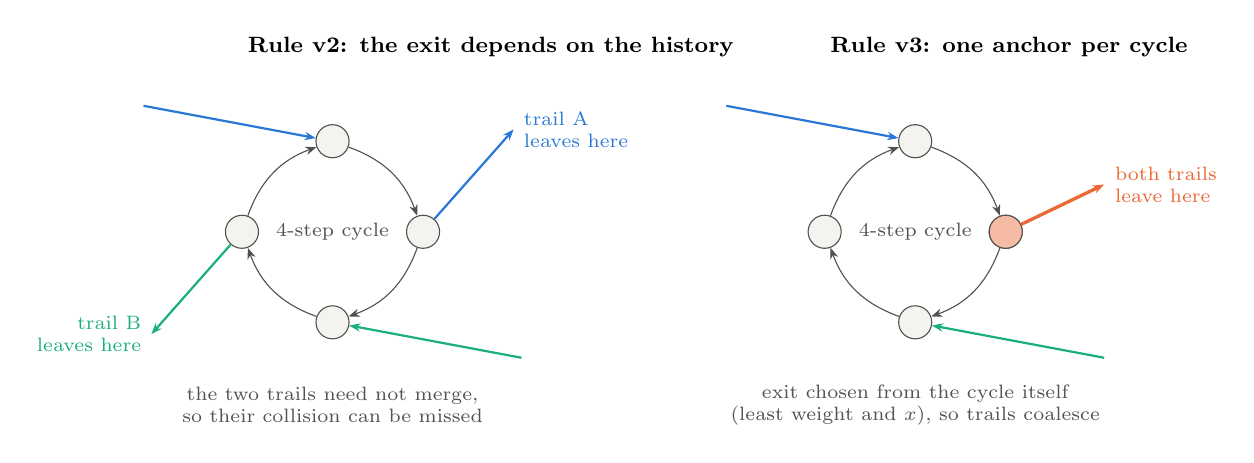
\begin{tikzpicture}[font=\scriptsize,
  pt/.style={circle,draw=inkS,fill=boxfill,inner sep=1.6pt,minimum size=0.42cm},
  anc/.style={pt,fill=cB!45},
  arr/.style={-{Stealth[length=4pt]},inkS},
  trA/.style={-{Stealth[length=4pt]},cA,thick},
  trB/.style={-{Stealth[length=4pt]},cC,thick},
]
\foreach \panel/\dx/\title in {0/0/{Rule v2: the exit depends on the history},1/7.4/{Rule v3: one anchor per cycle}}{
\begin{scope}[shift={(\dx,0)}]
\node[font=\footnotesize\bfseries,anchor=west] at (-1.2,2.35) {\title};
\foreach \i/\ang in {0/90,1/0,2/270,3/180}
  \node[pt] (c\panel\i) at (\ang:1.15) {};
\foreach \i/\j in {0/1,1/2,2/3,3/0}
  \draw[arr] (c\panel\i) to[bend left=25] (c\panel\j);
\node[font=\scriptsize,text=inkS] at (0,0) {4-step cycle};
\end{scope}}
% v2: two trails enter at different vertices and leave by different edges
\draw[trA] (-2.4,1.6) -- (c00);
\draw[trB] (2.4,-1.6) -- (c02);
\draw[trA] (c01) -- (2.3,1.3) node[right,align=left] {trail A\\leaves here};
\draw[trB] (c03) -- (-2.3,-1.3) node[left,align=right] {trail B\\leaves here};
\node[align=center,text=inkS] at (0,-2.2) {the two trails need not merge,\\so their collision can be missed};
% v3: both leave at the anchor (least key)
\node[anc] at (c11) {};
\draw[trA] (7.4-2.4,1.6) -- (c10);
\draw[trB] (7.4+2.4,-1.6) -- (c12);
\draw[trA,cB,very thick] (c11) -- (7.4+2.4,0.6) node[right,align=left] {both trails\\leave here};
\node[align=center,text=inkS] at (7.4,-2.2) {exit chosen from the cycle itself\\(least weight and $x$), so trails coalesce};
\end{tikzpicture}
\caption{Why the table walk's $20.08$ does not count. A table walk on
  Frobenius classes has short fruitless cycles that a trail must detect
  and leave. Under rule v2 the exit depended on how a trail arrived, so
  two trails entering the same cycle from different directions could
  leave by different edges and so fail to merge. Rule v3 confirms the cycle by
  walking it (at most eight raw steps) and leaves at one anchor chosen
  from the cycle's own points, so every trail entering it leaves the same
  way. The $\sigma$-walk has no fruitless cycles at all.}
\label{fig:cycles}
\end{figure}


Readers who skim the tables will see $20.08$ next to $15.88$ and
conclude that the table walk is the faster walk on Blackwell. Today
it is not, and the reason is correctness rather than arithmetic.

The table walk adds a precomputed point instead of a Frobenius image
of itself, which removes the basis conversions around $\sigma^j$ and
makes each step cheaper. The price is fruitless cycles: short loops
in which a trail returns to a class it has already visited and makes
no progress (Section~\ref{sec:walk-table}). The $\sigma$-walk has none
at all. Every table-walk rule is a way of noticing such a loop and
leaving it, and the rules have had three versions:
\begin{itemize}[leftmargin=1.2em,itemsep=0.2em]
\item \emph{v1}, as first built, let some cycle patterns through.
  The kernel ran at $16.56$~billion iterations/s on the RTX~PRO~6000
  and $5.55$ on the RTX~PRO~4500, but at campaign trail lengths it is
  modelled to trap about half of all trails, so its cost per solve is
  $4.85$--$6.26$ times the $\sigma$-walk's.
\item \emph{v2} closed those patterns, and the one-block build ran it
  at $20.08$ on the RTX~PRO~6000; the B200 sweep reached $19.40$ on a
  rule older than v3. A review then found that v2's exit from a cycle
  depended on the history a trail arrived with. Two trails entering
  the same cycle from different directions could leave it by different
  edges, which undermines the collision structure that rho relies on.
\item \emph{v3} fixes that. On a hint it follows at most eight raw
  steps, confirms an exact cycle, and leaves at one anchor chosen from
  the cycle itself, so every trail entering a cycle leaves it the same
  way. The probe sits on the critical path. The exact v3 kernel's
  first paired panel measured $5.10$~billion iterations/s on the
  RTX~PRO~6000~\evcite{\evref{v3}; \evref{client}, ``The earlier 20.078 B/s table result''}.
  On 2026-10-12 the fully tuned v3 build, which uses the same knob set
  as the $20.08$ build but now compiles rule v3, was screened at
  $8.24$ with its 300-report replay gate passing. That figure is a
  single unpaired screen, and the report that gives it does not carry
  its raw logs~\evcite{\evref{redesign}}. The $20.08$ receipt itself
  predates v3: its kernel had 116 registers and no stack frame, while
  the v3 probe needs 128 registers and a 400-byte
  frame~\evcite{\evref{oneblock}; \evref{v3}}.
\end{itemize}

So the honest summary is this. The $\sigma$-walk is the fastest
\emph{correct} walk we have on Blackwell, at $15.88$~billion iterations/s
on one RTX~PRO~6000 and $14.64$ in the audited campaign build. The table
walk is the faster \emph{arithmetic}: its v2 rate shows what the step
costs without the cycle probe, and that is the target for a faster
exact rule. Even a fast exact table walk only pays if its cost per
solve, which also depends on its walk constant, beats the
$\sigma$-walk's; under v2 that was projected at $0.81$--$0.86\times$ and has
never been measured. Section~\ref{sec:open-table} lists the routes we
see.

\subsection{RTX~PRO~4500}
\label{sec:g7}

The campaign's second GPU family is the RTX~PRO~4500 (82 SMs, 165~W)
in the AWS \texttt{g7.2xlarge}. We keep its ledger separate because on
this card the power cap binds, not the pipe. The shipping walk
measures $5.107$~billion iterations/s here at $1.95$~GHz, within about $1\%$ of what the
6000's per-SM-clock rate predicts (Section~\ref{sec:campaign-goal28}).
The card's own best preset before the map change sat near $6.2$~billion iterations/s.
Candidates such as the larger split batches were slower here because
they raised memory activity, and the power cap answered by lowering
the clock~\evcite{\evref{iterfn}, §6.3; \evref{client}, ``larger split-batch experiment''}.
We had declared a goal of $12$~billion iterations/s for this card
(Section~\ref{sec:campaign-goal28}), and it was reached by changing the
map rather than the kernel. The complete two-bridge $x$-only map of
Section~\ref{sec:walk-bridge} measured a median of $12.499203$~billion iterations/s
against $11.218437$~billion iterations/s for its matched modulus-32 control, a paired
geometric-mean ratio of $1.121079$ with $95\%$ interval
$[1.105668,\,1.136704]$. A fresh three-run confirmation gave
$12.567029$, $12.457221$ and $12.366415$~billion iterations/s, and the production build
ran at $12.632704$~billion iterations/s over $2^{36}$ updates~\evcite{\evref{client}, ``ECC2K-130 and ECC2K-95''; \evref{bridge}}.
We have not measured its DP34 collection rate on this card, so we do
not give one.

\subsection{GPU comparison}
\label{sec:survey}

Table~\ref{tab:survey} puts every part we measured side by side, with
the $\sigma$-walk and the table walk in separate columns. The
$\sigma$-walk column is one survey run of the same packed preset on
each Modal SKU (automatic workers, three valid \texttt{-{}-bench}
repeats, unpaired); the next column gives the best paired result on
that part, where one exists. The table-walk rates were all measured
under cycle rules older than the current v3, for the reason given in
Section~\ref{sec:sigma-vs-table}~\evcite{\evref{survey}; \evref{client}, ``Table-walk correctness update''}.

\begin{table}[t]
\centering
\footnotesize
\setlength{\tabcolsep}{4pt}
\caption{Rates in billions of iterations per second on one GPU.
  ``$\sigma$ survey'': the shipping packed preset, one unpaired Modal
  survey run (the RTX~PRO~4500 row is its AWS measurement). ``Best
  paired'': the best paired result on that part. ``Table, pre-v3'':
  table-walk rates under cycle rules v1 or v2, which are superseded
  (Section~\ref{sec:sigma-vs-table}); the exact v3 table walk measures
  $8.24$ on the RTX~PRO~6000 in an unpaired screen ($5.10$ in its first paired panel). ``M/SM'': million iterations per second per SM, our quotient of the
  survey rate by the SM count. ``T/\$'': trillions of iterations per dollar at
  Modal list price, 2026-09-19.}
\label{tab:survey}
\begin{tabular}{@{}llrrlrrr@{}}
\toprule
GPU & arch. & SMs & $\sigma$ survey & best paired & table (pre-v3) & M/SM & T/\$ \\
\midrule
RTX PRO 6000 & Blackwell \texttt{sm\_120} & 188 & 15.116 & 15.884 ($\sigma$, nibble table) & 20.078 (v2) & 80.4 & 17.95 \\
RTX PRO 4500 & Blackwell \texttt{sm\_120} & 82 & 5.107 & 12.499 ($x$-only bridge) & 5.552 (v1) & --- & --- \\
B200 & Blackwell \texttt{sm\_100} & 148 & 8.840 & --- & 19.402 & 59.7 & 5.09 \\
B300 & Blackwell \texttt{sm\_103} & 148 & 7.575 & --- & --- & 51.2 & 3.84 \\
H200 & Hopper \texttt{sm\_90} & 132 & 7.632 & --- & --- & 57.8 & 6.05 \\
H100 & Hopper \texttt{sm\_90} & 132 & 7.540 & --- & --- & 57.1 & 6.87 \\
L40S & Ada \texttt{sm\_89} & 142 & 8.696 & --- & --- & 61.2 & 16.04 \\
L4 & Ada \texttt{sm\_89} & 58 & 2.561 & --- & --- & 44.2 & 11.54 \\
A100-80GB & Ampere \texttt{sm\_80} & 108 & 4.632 & --- & --- & 42.9 & 6.67 \\
A100-40GB & Ampere \texttt{sm\_80} & 108 & 4.618 & --- & --- & 42.8 & 7.92 \\
A10 & Ampere \texttt{sm\_86} & 72 & 2.423 & --- & --- & 33.7 & 7.92 \\
T4 (no \texttt{clmad}) & Turing \texttt{sm\_75} & 40 & 0.541 & --- & --- & 13.5 & 3.30 \\
\bottomrule
\end{tabular}
\end{table}

\begin{figure}[t]
\centering
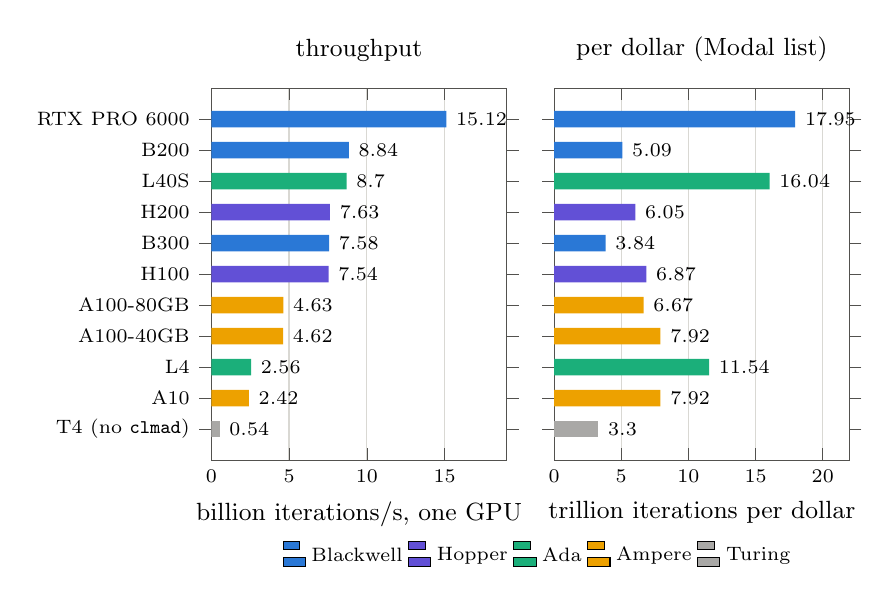
\begin{tikzpicture}
\begin{groupplot}[
  group style={group size=2 by 1, horizontal sep=0.6cm, yticklabels at=edge left},
  xbar, /pgf/bar width=6pt, /pgf/bar shift=0pt,
  width=0.44\textwidth, height=0.52\textwidth,
  symbolic y coords={p6000,b200,l40s,h200,b300,h100,a10080,a10040,l4,a10,t4},
  ytick={p6000,b200,l40s,h200,b300,h100,a10080,a10040,l4,a10,t4},
  yticklabels={RTX PRO 6000,B200,L40S,H200,B300,H100,A100-80GB,A100-40GB,L4,A10,T4 (no \texttt{clmad})},
  y dir=reverse,
  xmajorgrids, xmin=0,
  nodes near coords, nodes near coords style={font=\scriptsize,anchor=west},
  tick label style={font=\scriptsize},
]
\nextgroupplot[xmax=19, xlabel={billion iterations/s, one GPU}, title={\small throughput}]
\addplot[fill=cA,draw=none] coordinates {(15.116,p6000) (8.840,b200) (7.575,b300)};
\addplot[fill=cE,draw=none] coordinates {(7.632,h200) (7.540,h100)};
\addplot[fill=cC,draw=none] coordinates {(8.696,l40s) (2.561,l4)};
\addplot[fill=cD,draw=none] coordinates {(4.632,a10080) (4.618,a10040) (2.423,a10)};
\addplot[fill=inkS!50,draw=none] coordinates {(0.541,t4)};
\nextgroupplot[xmax=22, xlabel={trillion iterations per dollar}, title={\small per dollar (Modal list)},
  legend style={at={(-0.05,-0.2)},anchor=north,font=\scriptsize,draw=none},legend columns=5]
\addplot[fill=cA,draw=none] coordinates {(17.95,p6000) (5.09,b200) (3.84,b300)};
\addlegendentry{Blackwell}
\addplot[fill=cE,draw=none] coordinates {(6.05,h200) (6.87,h100)};
\addlegendentry{Hopper}
\addplot[fill=cC,draw=none] coordinates {(16.04,l40s) (11.54,l4)};
\addlegendentry{Ada}
\addplot[fill=cD,draw=none] coordinates {(6.67,a10080) (7.92,a10040) (7.92,a10)};
\addlegendentry{Ampere}
\addplot[fill=inkS!50,draw=none] coordinates {(3.30,t4)};
\addlegendentry{Turing}
\end{groupplot}
\end{tikzpicture}
\caption{The campaign's $\sigma$-walk on eleven GPUs, one survey run each
  with the same preset (Table~\ref{tab:survey}), by throughput and by
  iterations per dollar at Modal list price. The workstation Blackwell
  part leads on both; the data-centre Blackwell and Hopper parts run this
  integer-bound walk at about half its rate and a third of its value.}
\label{fig:gpus}
\end{figure}


Three things stand out. First, nothing beats the RTX~PRO~6000 on this
walk, per card, per SM or per dollar. It has the most SMs, a high
clock and Blackwell's unified integer lanes, and the walk is bound by
integer logic and the carry-less unit rather than by memory or tensor
cores, so the usual rankings of GPUs for machine-learning work do not
carry over: the B200 runs the $\sigma$-walk at $0.585\times$ the 6000 and
the H100 at half. Second, per SM, the Blackwell workstation die leads
the data-centre parts even though its carry-less unit is the slowest
in the table (Section~\ref{sec:blackwell-rates}), because the shipping
walk was tuned for exactly that balance. Third, the data-centre dies
reward a different kernel. With a table walk tuned for its fast
carry-less unit the B200 reaches $19.40$ (under a pre-v3 cycle rule),
more than twice its
$\sigma$-walk rate.

On the B200, an automatic sweep over twenty single-knob arms (launch
geometry, product form, scheduling, memory residency) later lifted the
table-walk build from $15.365$ to $19.402$~billion iterations/s ($1.2627$, every pair in
$1.2623$--$1.2632$). The winning combination of the fused pass, batch
32, three-limb Karatsuba and 512-thread blocks was adopted as
\texttt{gpu-b200-19b}. The same sweep on the 6000 found a $640\times1$
arm at $19.993$ against $19.951$, with two of five pairs below one, and
adopted nothing~\evcite{\evref{autosweep}}. The trades that change sign
from one die to the other are exactly those that move work from the
logic pipe onto the carry-less unit. The top-bit correction on
\texttt{CLMAD} costs $15\%$ on the 6000 but gains $13.4\%$ on the B200,
and stacked there with the normal-basis inversion and $\lambda^2$ on
\texttt{CLMAD} it reaches $1.379\times$ ($15.372$~billion iterations/s), just as the
per-die \texttt{CLMAD} rates of Section~\ref{sec:floor} predict. A
two-chain kernel that splits each warp's Montgomery chain in two lost
on both dies ($0.826\times$ on the B200, $0.696\times$ on the 6000),
which points to the register file rather than to any unit's
rate~\evcite{\evref{twochains}, §5, §6.2 and §6.4}.

\subsection{Rejected optimisations}
\label{sec:declined}

Table~\ref{tab:declined} lists every GPU candidate that we built,
measured against the rule, and did not adopt. We record them so that
anyone who has the same idea later finds a measurement rather than
folklore. Every row passed its correctness checks; what fell short was
the rate.

\begin{table}[t]
\centering
\small
\caption{GPU candidates measured and declined. Ratio is candidate
  over the paired control; intervals are $95\%$ paired bootstrap where
  the note reports one. ``4500'' rows are on the RTX~PRO~4500 against
  the selected runtime of the day; the others are on the RTX~PRO~6000.}
\label{tab:declined}
\begin{tabular}{@{}p{0.46\textwidth}rrl@{}}
\toprule
candidate & control & candidate & ratio \\
\midrule
stream Karatsuba compile option & $0.857$ & $0.748$ & $0.873$ \\
integer add in place of OR in \texttt{clmul32} & $6.8615$ & $6.8080$ & $0.992$ \\
top three-bit correction moved onto \texttt{CLMAD} & $15.116$ & $12.859$ & $0.851$ \\
batch 12 / 10 against batch 16 & $14.26$ & $13.75$ / $13.70$ & $<$ screen \\
batch 18 against batch 16 (larger population) & $14.47$ & $14.29$ & $<$ screen \\
table walk against pre-declared $17.0$~billion iterations/s & $14.41$ & $16.56$ & $1.149$, missed \\
two Montgomery chains per warp & $19.981$ & $13.903$ & $0.696$ \\
$\lambda$-projective coordinates (priced, not built) & --- & ceiling $11.8$--$12.5$ & $<14.41$ \\
4500: hybrid reduction & $6.2459$ & $5.3459$ & $0.852$ $[0.845, 0.860]$ \\
4500: half-native product tail & $6.1898$ & $6.0303$ & $0.977$ $[0.971, 0.982]$ \\
4500: quotient fan-in & $6.1739$ & $6.0139$ & $0.977$ $[0.972, 0.982]$ \\
4500: register-retained inverse, 3 / 4 blocks & $6.1724$ & $6.1487$ / $5.6922$ & $0.997$ / $0.924$ \\
4500: paired inverse leaves, 3 / 4 blocks & $6.1643$ & $6.1146$ / $5.6501$ & $0.994$ / $0.918$ \\
4500: logical-pair inversion, 3 / 4 blocks & $6.1675$ & $6.1037$ / $5.6723$ & $0.960$ / $0.921$ \\
4500: seven-node inversion, 3 / 4 blocks & $6.1826$ & $6.1388$ / $5.6904$ & $0.995$ / $0.923$ \\
4500: seven-node shared-$X$ cache, six slots & $6.2624$ & $6.3741$ & $1.010$ $[0.991, 1.029]$ \\
4500: split batch 24 / 32 & $6.2742$ & $6.1218$ / $5.9950$ & $0.972$ / $0.948$ \\
4500: direct polynomial $\delta$-3/4 routing & $6.2724$ & $4.3635$ & $0.690$ $[0.676, 0.704]$ \\
4500: 65/66-bit, 33-bit products; byte masks (four) & --- & --- & all $<1$ \\
\bottomrule
\end{tabular}
\end{table}

Sources: stream Karatsuba~\evcite{\evref{tuning}}; add-combine~\evcite{\evref{addcombine}};
top-\texttt{CLMAD}~\evcite{\evref{topclmad}}; batch
screen~\evcite{\evref{compact}}; two
chains~\evcite{\evref{twochains}}; $\lambda$-projective~\evcite{\evref{lambda}};
the 4500 rows~\evcite{\evref{client}, ``ECC2K-130 and ECC2K-95''}, each with
its own benchmark record.

Two rows need a word of explanation. The $\lambda$-projective
candidate was never built. Priced in the unit of
Table~\ref{tab:floor}, it came to $60.5$ \texttt{CLMAD} per update
against $38.1$ for affine at batch 16, a ceiling of $11.8$--$12.5$~billion iterations/s,
below the $14.41$ we had already measured. The condition we had
declared for building it (a negative cost difference at $W=16$) could
not be met, so we did not start. The top-\texttt{CLMAD} and
stream-Karatsuba rows are the two comparisons in this section that
were not interleaved on one allocation (the stream-Karatsuba pair also
differs in source digest). We report both with that caveat; neither
would have cleared the rule in any case.

\section{CPU}
\label{sec:cpu}

The CPU client matters for three reasons. Every GPU report is verified
on it, it runs the ECC2K-95 end-to-end control, and the campaign's spot
fleet included CPU workers whose points cannot be told apart from the
GPUs'. It is also where the instruction-set story of
Section~\ref{sec:isa} can be measured most directly, because the same
source compiles to scalar 64-bit words, AVX2, AVX-512 and NEON.

\begin{table}[t]
\centering
\small
\caption{Bitsliced CPU client, $\mathrm{GF}(2^{131})$, one core, median
  of five; M it/s is million iterations per second. Speedups are against
  the g++ 64-lane build on the same host. The Xeon's model is not
  recorded beyond its clock, and the record does not say whether the
  AVX2 row was built with AVX-512VL's ternary logic on 256-bit words. The 2009 qhasm implementation of Bailey et
  al.\ reached $533$ cycles per iteration on a Core~2 with 128-bit
  vectors.}
\label{tab:cpu}
\begin{tabular}{@{}llrrl@{}}
\toprule
host & word & lanes & M it/s & note \\
\midrule
Xeon 2.1~GHz & \texttt{uint64\_t} & 64 & 4.42 & 475 cycles/iteration \\
Xeon 2.1~GHz & AVX2 & 256 & 10.7 & 196 cycles/iteration \\
Xeon 2.1~GHz & AVX-512 & 512 & 12.6 & 167 cycles/it.; 4 threads 40~M \\
Graviton3 (V1, SHA3), clang & NEON & 128 & 6.214 & $2.38\times$ over g++/64 \\
Graviton2 (N1, no SHA3), clang & NEON & 128 & 4.220 & $2.09\times$ over g++/64 \\
Modal container, 4 threads & AVX-512 & 512 & 12.4 & 49.4~M on 4 threads \\
\bottomrule
\end{tabular}
\end{table}

\subsection{Bitsliced SIMD}
\label{sec:cpu-bitsliced}

Table~\ref{tab:cpu} collects the measurements~\evcite{\evref{client}, ``Throughput''},
and Figure~\ref{fig:cpu} draws them. A bitsliced client gains from a
CPU's vector extensions in two ways: wider words carry more walks per
instruction, and three-input logic fuses the XOR that follows every AND.
On x86 the step from 64-bit words to AVX2 is $2.4\times$ and AVX-512 adds
another $1.18\times$; AVX-512's \texttt{vpternlogd} is the CPU counterpart
of the GPU's \texttt{LOP3}. On Arm, a core without \texttt{FEAT\_SHA3}
(Graviton2) gets $1.81\times$ from the 128-bit NEON word and \texttt{BSL},
and a Graviton3, whose SHA3 extension adds the three-input \texttt{EOR3},
reaches $2.38\times$ its 64-bit build. On this code the compiler matters as much as
the instruction set: gcc emits $9{,}372$ instructions for the multiply
leaf, $59\%$ of them loads and stores of spilled temporaries, where clang
emits $1{,}902$ plus five outlined calls. We enable the SHA3 path only when
the CPU reports the feature: an ungated probe on a Graviton2 picks a
\texttt{+sha3} spelling under both compilers, and the binary dies with
\texttt{SIGILL} on its $8{,}907$ \texttt{eor3}
instructions~\evcite{\evref{client}, ``Word width''}.

The AVX-512 build's limit is data movement, not arithmetic. It spends
about half of each multiply on moves ($4{,}069$ logic instructions
against $4{,}287$ \texttt{vmovdqa32}), because the Karatsuba leaf keeps
254 values live with only 32 vector registers. A scheduling pass over
the same DAG recovered moves only in the conversion ($4{,}287$ to
$3{,}903$) and missed its declared target; repeated single-thread runs in
a shared container ranged from $15$ to $18.6$ million iterations per
second, too noisy for a throughput claim~\evcite{\evref{hostsched}}.

\subsection{Carry-less multiply}
\label{sec:cpu-clmul}

Every current CPU family also has a carry-less multiply: PCLMULQDQ and
its 512-bit form VPCLMULQDQ on x86, PMULL on Arm. The bitsliced client
deliberately does not use it. Its multiply leaf costs about 11
instructions per walk amortised over 512 lanes, while a per-walk 131-bit
carry-less product needs about nine \texttt{vpclmulqdq} plus a reduction
for a single walk~\evcite{\evref{hostsched}, §7}. A packed client is the
other design, the CPU twin of the GPU client: one walk per lane of
64-bit limbs, the product on the carry-less multiplier. The
\texttt{cryptanalysis} repository has one, using PMULL on Arm and
PCLMULQDQ on x86. It walks the table walk, not the campaign's
$\sigma$-walk, and has no measurement on the hosts reported
here~\evcite{\evref{cpupacked}}.

Two other CPU instructions were priced or measured on smaller binary
fields. GFNI's affine transform (\texttt{vgf2p8affineqb}) speeds up a
basis change $3$--$5\times$ for fields up to $2^{63}$ in the repository's
small-field code, but for ECC2K-130's bitsliced conversions it was
priced as a loss, since it acts on bytes inside a register where the
bitsliced maps act on whole words~\evcite{\evref{gfni}}. PCLMULQDQ made a
41-bit Koblitz rho $1.76\times$ faster end to end~\evcite{\evref{smallclmul}}.

The reference CPU rho of the repository's measurement harness, which
walks Frobenius classes on small Koblitz curves, was also tuned after
profiling. Canonicalising a point to its signed Frobenius class had
taken $54\%$ of a solve's instructions. Applying each normal-basis map
to both coordinates in one table pass, specialising the byte shapes of
the registered curves and sharing one modular reduction between the
two walk coefficients cut a complete solve on a 61-bit curve from
$1.995\cdot10^9$ to $1.601\cdot10^9$ instructions under Callgrind
($0.802\times$), against a pre-registered gate of $0.85$. Across 240
matched pairs on 48 targets the walks, recovered logarithms and every
counter were unchanged. This is an instruction count, not a rate: the
wall-time comparison could not run on a host with the required
isolation, and the change is not yet merged~\evcite{\evref{rhoopt}}.

\subsection{Prime fields}
\label{sec:cpu-prime}

The repository's prime-field CPU solver is a reference implementation,
not a fast one: it uses heap-allocated big integers, not four 64-bit
limbs with \texttt{MULX}/\texttt{ADX} carry chains or AVX-512 IFMA, and
manages about $32{,}000$ affine additions per second per thread on
P-256~\evcite{\evref{nistcpu}}. That is the CPU counterpart of the gap the
GPU closed with explicit carry chains (Section~\ref{sec:nist}), and it is
listed as an open question in Section~\ref{sec:open-cpu}.

\subsection{CPUs in the campaign}
\label{sec:cpu-fleet}

In the campaign a CPU worker was a whole multi-core instance, and the
twelve CPU slots self-reported a median of $2.3$ billion iterations per
second on 2026-09-17, about a sixth of an RTX~PRO~6000. On Modal, a
32-thread (16-core) sidecar beside a GPU adds about $25\%$ to the
container's cost for $2.7\%$ more iterations, so it is off by
default~\evcite{\evref{dpint}; \evref{client}, ``Walking on the container's CPUs too''}.
Per dollar, a CPU walker is roughly ten times worse than the GPU.

\begin{figure}[t]
\centering
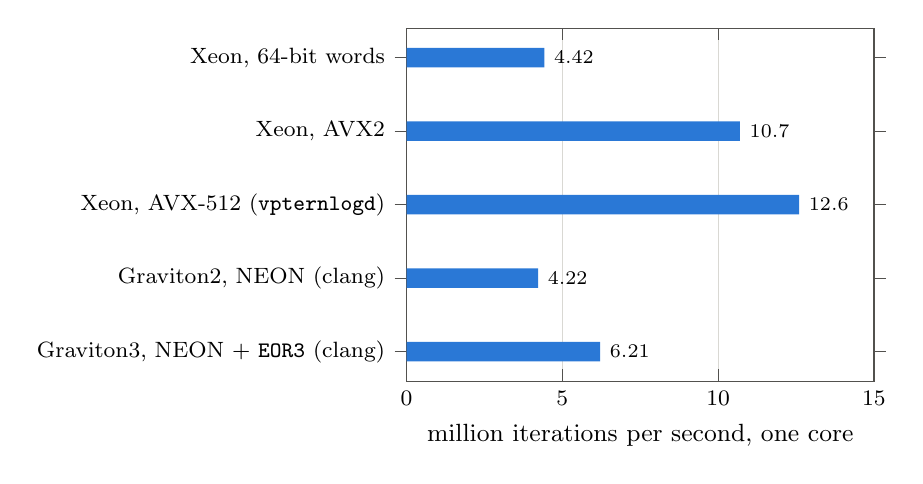
\begin{tikzpicture}
\begin{axis}[
  xbar, bar width=7pt, bar shift=0pt,
  width=0.62\textwidth, height=0.5\textwidth,
  xmin=0, xmax=15,
  xlabel={million iterations per second, one core},
  symbolic y coords={x64,xavx2,xavx512,g2,g3},
  ytick={x64,xavx2,xavx512,g2,g3},
  yticklabels={
    {Xeon, 64-bit words},
    {Xeon, AVX2},
    {Xeon, AVX-512 (\texttt{vpternlogd})},
    {Graviton2, NEON (clang)},
    {Graviton3, NEON + \texttt{EOR3} (clang)},
  },
  y dir=reverse,
  xmajorgrids,
  nodes near coords, nodes near coords style={font=\scriptsize,anchor=west},
  legend style={at={(0.5,-0.2)},anchor=north},
  legend columns=2,
  legend cell align=left,
]
\addplot[fill=cA,draw=none] coordinates {(4.42,x64) (10.7,xavx2) (12.6,xavx512)
  (4.220,g2) (6.214,g3)};
\end{axis}
\end{tikzpicture}
\caption{CPU rates per core by instruction set. Bitsliced rows are the
  campaign walk (Table~\ref{tab:cpu}); each step down a group adds one
  extension.}
\label{fig:cpu}
\end{figure}


\section{NIST curves}
\label{sec:nist}

Most of what made the ECC2K-130 client fast has nothing to do with
binary fields. Sharing one inversion across many walks, using the
hardware's own carry instructions instead of emulating them, choosing
the launch shape by measurement, and refusing occupancy trades that
look good on paper are all properties of an affine-addition rho walk
on a GPU, not of $\FF_{2^{131}}$. So once the ECC2K-130 ladder was
written down, the natural question was how much of it carries over to
a prime-field walk. We tried it on NIST P-256 and P-384, on the same
RTX~PRO~6000, and this section reports what happened.

Two things should be clear before the numbers. First, these are
throughput measurements on a walk that nobody expects to finish: at
the rates below a P-256 collision is still about $2\cdot10^{29}$ seconds
away (Section~\ref{sec:solvetime-nist}), and nothing here says anything about the security of the NIST
curves. Second, every row is engineering in the sense of
Section~\ref{sec:intro}. The walk computes the same function on the
same curve at every rung, with one step per counted step, so
$S=\text{steps}/\sqrt n$ does not move; only the cost of a step
does~\evcite{\evref{nistres}}.

\subsection{Walk and field}
\label{sec:nist-walk}

The library holds a P-256 element in eight 32-bit limbs and a P-384
element in twelve, one element per thread, with CIOS Montgomery
multiplication. Both primes have low limb $2^{32}-1$, so the Montgomery
constant is $n'=1$, and every limb of either modulus in radix $2^{32}$
is $0$, $1$, $2^{32}-1$ or $2^{32}-2$; the reduction row therefore
needs carries but no multiplications. A generalised-Mersenne (Solinas)
field is kept alongside as a matched competitor, so that the device
rather than an argument decides between the two~\evcite{\evref{nist}}.
Both representations are checked on $20{,}000$ random pairs per curve
against Boost.Multiprecision, and the Jacobian doubling and mixed
addition against independent affine arithmetic. The benchmark
protocol was pre-registered before any device time: workloads, seeds,
the threads-per-block and register-cap sweep, and a $5\%$ threshold
below which the simpler configuration wins by
rule~\evcite{\evref{nistproto}}.

The rho walk on top of the field mirrors the structure of
Section~\ref{sec:walk}, minus the Frobenius. It is an $r$-adding walk
on the low bits of $x$ with the negation map as the only fold (fold~2,
a $\sqrt2$ saving; $j\neq0$ on both curves, so $\pm1$ is the whole
automorphism group), distinguished points by a mask on the next byte
at probability $2^{-24}$, fruitless two-cycles detected and escaped,
and walks batched per thread so that one inversion serves all of
them through Montgomery's trick~\evcite{\evref{nist}}. The
inversion is Fermat's $a^{p-2}$ with a four-bit fixed window, which
for P-256 is on the order of 256 squarings and 64 window
multiplications (our count from the exponent length, not a measured
figure). That is the important difference from the binary field. On
ECC2K-130 an inversion costs eight multiplications because squaring is
free (Section~\ref{sec:arith}); here it costs a few hundred, so the
batch width $W$ matters far more.

The host test suite runs the exact kernel body on the CPU: group-law
identities, determinism of a single step, the negation fold as a
class function, and an end-to-end logarithm on a toy curve of order
about $2^{20}$, where the folded walk needs the expected $\sqrt2$
fewer steps than the unfolded one~\evcite{\evref{nist}, ``Correctness''}.

\paragraph{The CPU solver across all fifteen curves.} The GPU walk has a CPU
counterpart: a host solver that takes any of the fifteen FIPS~186-4
curves (P-192 to P-521, K-163 to K-571, B-163 to B-571), audits it
for the structural precondition of each known attack (trace one,
composite order, embedding degree at most 100, composite extension
degree), and runs the branch the curve calls for:
Smart--Semaev--Satoh--Araki, Pohlig--Hellman, interval baby-step
giant-step and kangaroo, or whole-group rho. The audit certifies the
absence of every precondition on all fifteen. The rho folds the
negation map everywhere and the Frobenius on the Koblitz curves, the
class of size $2m$ carried exactly through the eigenvalue $\lambda$
of $\tau$ on the subgroup, which is the binary-curve cousin of the
$\sigma$-class walk of Section~\ref{sec:walk}. On one host we measured
interval solves of width $2^{20}$ to $2^{32}$ on P-256, K-283 and
B-409 in $43$~ms to $8.7$~s with the planted scalar recovered every
time; Frobenius folding on toy Koblitz curves cutting additions by
the predicted $\sqrt{2m}$ ($6.8\times$ at $m=23$, $9\times$ at
$m=41$) at a cost of $m$ squarings per step; and the Smart attack
breaking CM-constructed anomalous curves of 129, 257 and 522 bits in
3, 10 and 33~ms. No full-width scalar has been recovered on any NIST curve, and
none of the fifteen has a structural weakness; the documentation says
both~\evcite{\evref{nistcpu}}.

\subsection{Baseline}
\label{sec:nist-first}

The kernel had been written and verified entirely on hosts without a
GPU (Section~\ref{sec:othergpu-status}), and the first device run
measured nothing at all. The batched-inversion routine was marked
host-only, and \texttt{nvcc}, after a warning, silently dropped the
call from device code. The walk kernel compiled to a load and an exit:
four registers, no stack, microseconds per launch and zero
distinguished points. The CPU tests could not have caught it, because
the host compiler happily compiles host-only code. A second bug, an
unguarded \texttt{atomicAdd} on a null cycle counter, faulted on the
first fruitless two-cycle, which arrives about once every 512 steps.
Both are fixed and now covered by tests, and the device benchmark
checks every launch for errors~\evcite{\evref{nistres}, ``What this round fixed''}.

This is the same lesson that Section~\ref{sec:arith-bitsliced} drew
from code size, in a different form: a static count or a host
emulation tells you what the device ought to do, and only the device
tells you what it did. Our correctness check on hardware is therefore
the distinguished-point count. Because the walk is deterministic and
points are distinguished with probability $2^{-24}$, every cell must
report about $\text{walks}\times\text{iterations}/2^{24}$ of them.
Every cell did, for example $11{,}969$ observed against $12{,}085$
expected on the first P-256 run and $12{,}154$ against $12{,}096$ in
the best cell~\evcite{\evref{nistres}, ``Correctness evidence on hardware''}.
The CPU suite also checks the specialised steppers below bit for bit
against the generic one, for every batch width that was compiled.

\subsection{Optimisations}
\label{sec:nist-rungs}

Table~\ref{tab:nist-ladder} lines the NIST rungs up against the
ECC2K-130 rungs they borrow from. The starting point is the portable
build at 128 threads per block and $W=8$: $1.075$~billion iterations/s on P-256
and $0.210$ on P-384, both on one RTX~PRO~6000 Blackwell (188 SMs,
CUDA~13.3, \texttt{sm\_120}).

\begin{table}[t]
\centering
\small
\caption{ECC2K-130 levers applied to the NIST P-256 and P-384 rho walk
  on one RTX~PRO~6000. Rates are in billions of iterations per second. Each NIST ratio compares
  adjacent cells of the same sweep; the cells are single runs, not the
  interleaved repeated pairs of Section~\ref{sec:gpu}. Rows marked
  $^\ast$ come from the round-2 sweep. Class: engineering.}
\label{tab:nist-ladder}
\begin{tabular}{@{}>{\raggedright\arraybackslash}p{0.25\textwidth}>{\raggedright\arraybackslash}p{0.21\textwidth}>{\raggedright\arraybackslash}p{0.20\textwidth}rr@{}}
\toprule
NIST rung & ECC2K-130 analogue & cells compared & P-256 & P-384 \\
\midrule
first working build & bitsliced control & portable, 128 thr., $W=8$ & $1.075$ & $0.210$ \\
\addlinespace
explicit PTX carry chains & native \texttt{clmad} ($+22.4\%$) & same cell, PTX build & $1.19\times$ & $1.38\times$ \\compile-time $W$, $W=8\to16$ & batch tuning ($+52\%$) & 256 thr., PTX & $1.08\times$ & $1.37\times$ \\
128 $\to$ 256 threads/block & launch geometry ($+9.4\%$) & $W=16$, PTX & $1.03\times$ & $1.01\times$ \\
$W=32$, register-resident inversion$^\ast$ & batch tuning & 256 thr., $W=16\to32$ & $1.22\times$ & $1.31\times$ \\
register caps 96/128/160$^\ast$ & two chains, blocks/SM (declined) & 256 thr., $W=32$ & $0.97\times$ & $0.82$--$0.83\times$ \\
\midrule
best cell$^\ast$ & & PTX, 256 thr., $W=32$ & $\mathbf{1.632}$ & $\mathbf{0.548}$ \\
cumulative$^\ast$ & & from the first working build & $\mathbf{1.52\times}$ & $\mathbf{2.61\times}$ \\
\bottomrule
\end{tabular}
\end{table}

\paragraph{Carry chains.} On ECC2K-130 the single largest
instruction-level gain was letting the hardware do the carry-less
product itself. The prime-field counterpart is the carry: a portable
C++ multi-precision product hides its carries in compares and adds,
and Section~\ref{sec:othergpu-fp256} already showed that the
256-bit product is carry-bound rather than multiply-bound. Writing the
product rows and the sparse reduction with explicit
\texttt{mad.lo.cc}/\texttt{madc.hi.cc} chains lifted the walk by
$1.19\times$ on P-256 and $1.38\times$ on P-384 at the same launch
shape ($1.282$ and $0.289$~billion iterations/s). The larger gain on P-384 is what
one would expect from twelve limbs instead of eight: there are more
carries per product to save. At the field level the same change took
a dependent Montgomery multiply from $54.9$ to $73.4$~billion multiplications/s on P-256 and
from $20.3$ to $32.2$~billion multiplications/s on P-384. Under the pre-registered protocol the Solinas competitor did not
win either. On P-256 the two multiplications are within $5\%$ ($70.4$
against $73.4$~billion multiplications/s), a tie that the protocol
awards to the simpler configuration. On P-384 the Solinas
multiplication is $14\%$ faster ($36.7$ against $32.2$) but the
Montgomery doubling is $4\%$ faster ($1{,}712$ against $1{,}647$~million
doublings/s). These field rows are a first run at one block size, not
the protocol's three repeats, so the question stays
open~\evcite{\evref{nistres}, ``Field arithmetic''}. The walk is built
on the Montgomery field for both curves; a Solinas walk has not been compiled or measured~\evcite{\evref{nist}}.

\paragraph{Batch width.} This is where the two fields differ most,
and the reason is the inversion. On ECC2K-130 the batch went
\emph{down}, from 32 walks per inversion to 16, because an inversion
was already cheap and a smaller hot state fitted the cache better. On
the NIST curves an inversion costs hundreds of multiplications, so
every extra walk sharing it pays. Templating the stepper on $W$ at
compile time let the per-walk arrays live in registers instead of
64-wide local arrays, and the rate climbed with $W$ on every
geometry: at 256 threads per block from $0.466$ at $W=2$ to $1.340$ at
$W=16$ on P-256, and from $0.096$ to $0.438$ on P-384
(Figure~\ref{fig:nist-w})~\evcite{\evref{nistres}, ``Rho walk''}. A
second round passed the inversion's scratch arrays by reference and
compiled a $W=32$ instance. That cell reached $1.632$ and
$0.548$~billion iterations/s, $1.22\times$ and $1.31\times$ over $W=16$ at the
same geometry~\evcite{\evref{nistres}, round 2}.
We cannot cleanly split that gain between the larger batch and the
by-reference inversion, because round 1 never compiled $W=32$. What we
can say is that at $W\le16$ the two rounds agree within noise
($1.306$/$0.434$ against $1.310$/$0.408$ at 128 threads, $W=16$), which
suggests, without proving it, that most of the gain comes from the
batch.

\paragraph{Launch shape.} Doubling threads per block from 128 to 256
was worth $2.6\%$ on P-256 and under $1\%$ on P-384 at $W=16$. That is
small next to the one-block geometry's $9.4\%$ on ECC2K-130, and it
makes sense: the binary kernel was shaped by a shared-memory table and
an L1 budget, while the prime-field walk is limited by registers.

\paragraph{Rejected changes.} At $W=32$ both instantiations sit at
the 255-register ceiling. The standard counter-measure is a register cap,
trading spills for occupancy, and the round-2 sweep tried caps of 96,
128 and 160 registers. All of them lost to the unrestricted build:
P-256 fell to $1.589$--$1.595$ and P-384 to $0.447$--$0.455$. That
matches the ECC2K-130 experience with the two-chain kernel and the
four-block configurations of Table~\ref{tab:declined}: on this card,
occupancy bought with spilled state has not paid on either field.

\begin{figure}[t]
\centering
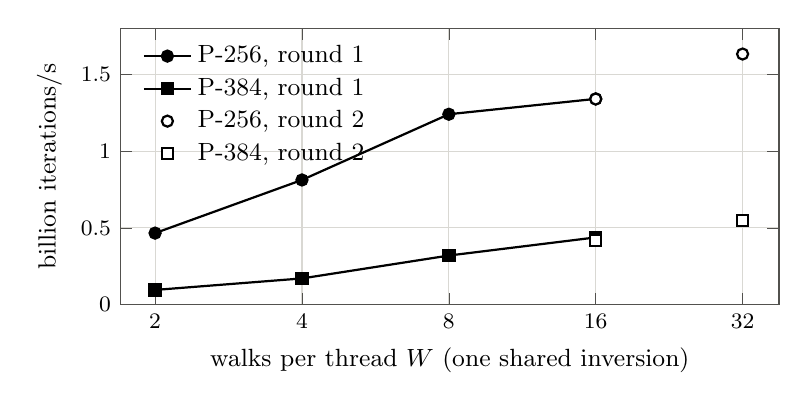
\begin{tikzpicture}
\begin{axis}[
  width=0.82\textwidth,
  height=0.42\textwidth,
  xlabel={walks per thread $W$ (one shared inversion)},
  ylabel={billion iterations/s},
  xmode=log, log basis x=2,
  xtick={2,4,8,16,32},
  xticklabels={2,4,8,16,32},
  xmin=1.7, xmax=38,
  ymin=0, ymax=1.8,
  grid=major,
  legend style={at={(0.02,0.98)},anchor=north west,font=\small},
]
\addplot[mark=*,thick] coordinates {
  (2,0.466) (4,0.812) (8,1.24) (16,1.340)
};
\addlegendentry{P-256, round 1}
\addplot[mark=square*,thick] coordinates {
  (2,0.096) (4,0.171) (8,0.32) (16,0.438)
};
\addlegendentry{P-384, round 1}
\addplot[mark=*,only marks,mark options={fill=white},thick] coordinates {
  (16,1.339) (32,1.632)
};
\addlegendentry{P-256, round 2}
\addplot[mark=square*,only marks,mark options={fill=white},thick] coordinates {
  (16,0.417) (32,0.548)
};
\addlegendentry{P-384, round 2}
\end{axis}
\end{tikzpicture}
\caption{The NIST rho walk on one RTX~PRO~6000 at 256 threads per block,
  PTX build, unrestricted registers, against the batch width $W$.
  Filled markers are the round-1 sweep, open markers the round-2 sweep
  with the by-reference inversion and the $W=32$ instance. Each point
  is one cell of $8{,}192$ iterations; distinguished-point counts
  matched the $2^{-24}$ rate in every cell.}
\label{fig:nist-w}
\end{figure}

\subsection{Transfer from ECC2K-130}
\label{sec:nist-lessons}

Three of the ECC2K-130 levers transferred directly. Native carry
handling, batch width and the refusal of register caps all moved the
NIST walk in the same direction they moved the binary one, and the
combined effect was $1.52\times$ on P-256 and $2.61\times$ on P-384 over
the first working build. The size of each lever did not transfer. The
batch width, a modest knob on ECC2K-130, was the largest single factor
here because a prime-field inversion takes some forty times as many
multiplications as a normal-basis one. Launch geometry, a real gain on the
binary walk, was nearly flat. In other words the ladder carried over,
but its rungs were spaced differently, and the only way to find the
spacing was to measure it.

The comparison also puts the two walks on one scale. On the same card
the ECC2K-130 campaign build runs $14.64$ billion complete iterations
per second and the best P-256 walk $1.63$ billion iterations, a factor of
about nine. A 131-bit binary product is six \texttt{CLMAD}
instructions; a 256-bit prime product is two hundred or so
carry-chained integer instructions (Table~\ref{tab:fp256}). That
factor of nine is the carry-less unit's advantage made concrete.

The next candidate steps are the ones the round-2 record names: a $W=64$
instance (which will spill at the register ceiling and probably lose,
but is worth one cell to confirm), reseeding off the critical path,
and a second walk per step from the same table read. A repeated,
interleaved pairing of the best cell against its control, in the
style of Section~\ref{sec:gpu}, would also turn these single-run
ratios into intervals. None of that changes the exponent, and none of
it is meant to.

\section{Other GPU kernels}
\label{sec:othergpu}

The ECC2K-130 client is one of several GPU arithmetic libraries in
the two repositories. The others target the 256-bit prime field of
secp256k1 (a Koblitz curve in the SEC sense, with $j=0$ and the
order-3 endomorphism), the NIST primes and the polynomial-basis field of
ECC2K-95. They follow the same discipline as the
ECC2K-130 client: a Python or Rust oracle, a host emulation of the
identical device source, bit-identical steppers, planted logarithms,
and static instruction accounting from the assembler. What most of
them still lack is a measurement on a device. We start by saying
which is which, because a static instruction count and a measured
rate are different kinds of evidence, and the rest of the paper keeps
them apart.

\subsection{Status}
\label{sec:othergpu-status}

\begin{table}[t]
\centering
\small
\caption{GPU arithmetic in the two repositories by evidence class.
  ``Emulated'' means the device source was executed on the host and
  checked against an oracle; ``static'' means instruction, register
  and stack counts from \texttt{ptxas} with no execution.}
\label{tab:gpu-status}
\begin{tabular}{@{}p{0.30\textwidth}p{0.17\textwidth}p{0.22\textwidth}p{0.22\textwidth}@{}}
\toprule
kernel family & field & on a device & otherwise \\
\midrule
ECC2K-130 client (Sections~\ref{sec:gpu}, \ref{sec:campaign}) & $\FF_{2^{131}}$, ONB & measured, audited & emulated, static \\
secp256k1 / Curve25519 rho, baby-step giant-step & $\FF_p$, two 256-bit primes & never & emulated, static \\
secp256k1 kangaroo & $\FF_p$, 256-bit & never & emulated, static \\
P-256 / P-384 field and rho walk (Section~\ref{sec:nist}) & $\FF_p$, 256- and 384-bit & measured (RTX PRO 6000, 2026-10-12) & host-verified; protocol pre-registered \\
ECC2K-95 kernel & $\FF_{2^{97}}$, polynomial basis & never & emulated, static \\
64-bit prime-field rho (\texttt{cryptanalysis}) & $\FF_p$, $p<2^{64}$ & never & emulated, static \\
\bottomrule
\end{tabular}
\end{table}

Table~\ref{tab:gpu-status} is the inventory. Every ``never'' repeats a
sentence in that family's own README, and the reason is the same each
time: the code was written and verified in containers with no GPU or
no complete CUDA toolkit, and the device runs were planned for rented
hardware that the campaign's account hold
(Section~\ref{sec:campaign-state}) or missing credentials then put out
of reach. The NIST kernels were in the same position until they
finally ran, which is the subject of Section~\ref{sec:nist}~\evcite{\evref{ecc}; \evref{kangaroo}; \evref{ecc2k95}; \evref{nistattempt}; \evref{prho64}, ``How this is tested''}.
The numbers below are therefore of two kinds, and we label each one: a
static count, or an emulated operation count or walk constant.

\subsection{secp256k1}
\label{sec:othergpu-fp256}

The field layer holds an element in eight 32-bit limbs, because the
integer datapath is 32 bits wide and the carry-chain instructions
\texttt{mad.lo.cc}, \texttt{madc.hi.cc} and \texttt{addc} exist only at
that granularity. For secp256k1 the 512-bit product is folded with
$2^{256}\equiv2^{32}+977 \pmod p$, about $40\%$ fewer multiply-adds
than Montgomery; for any other odd modulus below $2^{256}$ a
Montgomery CIOS path is used, and the scalar ring modulo $n$ reuses
it on the host. Points are Jacobian with the standard $a=0$ doubling
($2M+5S$) and mixed addition ($7M+4S$) formulas. The library is a
throughput library, not a signing library, and is not
constant-time~\evcite{\evref{ecc}; \evref{ecc}}.
A second special-reduction path, added in October 2026, serves
Curve25519 (Ed25519's prime-order group in short-Weierstrass form,
$p=2^{255}-19$, folded with $2^{256}\equiv38$) through the same
walk, baby-step giant-step and test suites; it is host-verified
against the RFC~7748 constants and has not run on a
device~\evcite{\evref{ecc}}.

\begin{table}[t]
\centering
\small
\caption{Static PTX instruction counts for one 256-bit field
  multiplication (clang, \texttt{sm\_90}, \texttt{-O3}). The hard floor
  for the product is 128 instructions: 64 limb products at two
  instructions each. Class: engineering; nothing here has executed on
  a device.}
\label{tab:fp256}
\begin{tabular}{@{}lrrr@{}}
\toprule
 & portable C++ & inline PTX, before & inline PTX, after \\
\midrule
512-bit product & 236 & 171 & 137 \\
secp256k1 reduction & 146 & 130 & 77 \\
full multiply & 472 & 328 & \textbf{210} \\
\midrule
Montgomery CIOS multiply & 475 & --- & 352 \\
\bottomrule
\end{tabular}
\end{table}

Table~\ref{tab:fp256} is the instruction ledger. The portable path
emits no carry instructions at all: of the 444 instructions in a
portable squaring, 178 are adds, 102 shifts, 100 ANDs and only 46
multiplies, so the multiply is carry-bound, not multiply-bound, and
the inline-PTX rewrite's $55\%$ cut comes from the carry chains. The
seven assembly blocks are checked by an interpreter against the
portable path on $20{,}000$ random and boundary inputs each, and that
check is mutation-tested; it does not cover register allocation or
device semantics, which is why \texttt{FP\_PTX} is off by
default~\evcite{\evref{eccopt}, §2; \evref{ecc}}.

In the unit of Section~\ref{sec:arith}, a secp256k1 inversion is 270
multiplications (255 squarings and 15 multiplications along the
libsecp256k1 addition chain), a rho step with batch $W$ is $6+270/W$
multiplications ($3$ for the affine addition, $3$ for Montgomery's
trick), $7+270/W$ with the $j=0$ fold: $39.8$ at $W=8$, $14.4$ at
$W=32$, $8.1$ at $W=128$, against 276 unbatched~\evcite{\evref{eccopt}, §1}.
Three things were tried and declined on the static count: a
dedicated squaring routine ($-2.7\%$ portable, $+23.5\%$ on the PTX
path; reverted), lazy reduction to $[0,2^{256})$ (worth about $10\%$
of a multiply, but it breaks the canonical form that equality, the
distinguished-point test, the cycle hash and the fold comparison rely
on), and Karatsuba (judged to lose on a carry-bound multiply). Tensor
cores were considered and not reached for~\evcite{\evref{eccopt}, §2 and §4.4}.
Marking the inversion and ladder routines \texttt{\_\_noinline\_\_}
and replacing two 16-entry tables by a small double-scalar ladder
took the walk kernel's stack from $4{,}664$ to $1{,}616$~B (the
low-memory variant from $4{,}008$ to $792$~B) and the compile from
over ten minutes to 46~s, the same code-size lesson as
Section~\ref{sec:arith-bitsliced}~\evcite{\evref{eccopt}, §3}.

\subsection{Automorphism folding and BSGS}
\label{sec:othergpu-rho}

The rho walk is $r$-adding on the low bits of $x$, with distinguished
points by a mask on the next byte and three folds: identity, the
negation map, and on $j=0$ curves the full $\langle\beta,-1\rangle$
orbit of order six, chosen by minimising $x$ over
$\{x,\beta x,\beta^2 x\}$ at the cost of one multiplication
($\beta^2x=-(x+\beta x)$) and two compares, about $10\%$ of a batched
step for $\sqrt3$ fewer steps. Only an automorphism code is kept per
step; a report is $\{x,\text{walk},\text{restart},\text{steps}\}$, 48
bytes, and the host replays the two colliding walks from their seeds,
multiplying $(a,b)$ by $(-1)^{\text{neg}}\lambda^k$ at each step. Fruitless
cycles of length 2 to 6 are detected with a five-deep ring and escaped
by doubling the member with the smallest hash; their measured rates
at $R=8$ agree with the prediction to about
$10\%$~\evcite{\evref{ecc}, ``The walk''}.

On a 36-bit $j=0$ toy curve in host emulation (8 solves per fold, 16
walks, $R=256$, period $2^7$), the mean steps were $305{,}740$,
$199{,}042$ and $113{,}522$ for folds 1, 2 and 6 against predictions of
$249{,}454$, $176{,}391$ and $101{,}839$ ($1.23\times$, $1.13\times$,
$1.11\times$; $\pm0.18\times$ on a mean of eight), all $8/8$ correct,
so fold 6 buys $1.75\times$ over the negation map (predicted $1.73$).
In the unit $S=\text{ops}/\sqrt n$ that is $1.54$, $1.00$ and $0.57$.
The three steppers (batched, low-memory, one-inversion-per-walk) are
bit-identical over hundreds of iterations with the same
distinguished-point multiset, and every point replays on the host to
$aP+bQ$, which is what proves the $\lambda$ bookkeeping on secp256k1
itself~\evcite{\evref{ecc}, ``How this is tested''}.

Baby-step giant-step on the same arithmetic keeps an $x$-keyed table
of 16-byte entries in lock-free open addressing (one 64-bit
\texttt{atomicCAS} per probe, about $2.5$ slots per probe at half
load, a false-candidate rate of load$/2^{32}$ and none observed), and
walks $W$ giant chains per thread sharing one inversion, 94 registers
and no spills at $W=8$. With the negation map the layout is $m=\sqrt{w}/2$
babies and $2m-1$ giants, the Galbraith--Wang--Zhang row at $1.00\sqrt w$
expected against the textbook $1.41\sqrt w$. A $2^{66}$-wide interval
is $2^{32}$ entries and 64~GB, the top of one 80~GB device; beyond
that the method is out of memory, not out of
time~\evcite{\evref{ecc}, ``Baby-step giant-step''}.
Table~\ref{tab:bsgs} is the measured cost on a 40-bit toy curve, in
emulation, every phase charged.

\begin{table}[t]
\centering
\small
\caption{Rho and baby-step giant-step on a 40-bit toy curve
  ($n=649{,}523{,}094{,}257$), host emulation of the device source, 128
  chains, mean over 8 random targets. $S=\text{group additions}/\sqrt n$
  with table construction charged. The rho rows predate the order-six
  fold and were single solves ($\pm0.5\times$). Twelve targets on a
  $2^{26}$ interval cost $S=0.560$ per target against $2.131$ for one
  cold solve.}
\label{tab:bsgs}
\begin{tabular}{@{}lrrrl@{}}
\toprule
row & table$/\sqrt n$ & mean $S$ & predicted & correct \\
\midrule
rho, negation map (reference) & 0 & 0.85 & --- & 1/1 \\
rho, no negation map & 0 & 1.42 & --- & 1/1 \\
BSGS textbook, reference stepper & 0.707 & 1.44 & 1.41 & 21/21 \\
BSGS textbook, batched $W=16$ & 0.707 & 1.44 (bit-identical) & 1.41 & 21/21 \\
BSGS negation layout, $W=16$ & 0.500 & 1.07 & 1.00 & 21/21 \\
\quad giant phase only & 0.500 & 0.56 & 0.50 & 8/8 \\
\bottomrule
\end{tabular}
\end{table}

The classification is the same as every row in Section~\ref{sec:gpu}:
the batched stepper is engineering, the layouts are the published
ones, and nothing moves the ratio to the generic floor. A Rust port of
the same baby-step giant-step on the CPU runs at $37$--$49$~M
steps/s on four threads at $S=1.03$ cold and $0.55$ amortised, $6$--$11\times$
the big-integer implementation it replaced~\evcite{\evref{ecc}, ``Cost, measured''}.
The emulation itself runs at about $380$~k steps/s per core, a
figure that says nothing about a device and is quoted only so that
no one mistakes it for one.

\subsection{Kangaroo}
\label{sec:othergpu-kangaroo}

The interval solver reuses the verified field and point code for
$Q=kG$ with $k\in[a,a+w)$ at about $2\sqrt w$ steps: two herds that
alternate by thread parity so every warp is half tame and half wild,
a jump table of $2^6$ pseudo-random scalars with mean jump $\sqrt w/2$
and 25-word entries (odd, so the shared-memory reads are
bank-conflict-free), and the target centred at $Q'=Q-(a+w/2)G$. The
invariant that makes it testable is that after every step a tame
kangaroo at distance $d$ is at $dG$ and a wild one at $Q'+dG$, which
pins the jump table, the distance accumulator and the point
arithmetic together~\evcite{\evref{kangaroo}, ``How the walk works''}.

Its measured constant is the useful number. In emulation on a $2^{31}$
interval with 120 trials per configuration, steps are $C\sqrt w$ with
$C=2.79\pm0.13$ for the default (median $2.65$); the idealised
two-herd bound is $2.0$, Pollard's classic lambda about $3.3$, and
published parallel implementations about $2.1$, so this one is about a
third above the best published. A jump-parameter sweep at 20 trials
per cell had shown $C$ from $2.50$ to $3.95$, an apparent $36\%$ win;
rerun at 120 trials the best cell and the default were within half a
standard error. The defaults sit on a flat optimum and the sweep was
noise, which is recorded so that it is not rediscovered. Restarting
at a distinguished point or not was likewise within
noise~\evcite{\evref{kangaroo}, ``Measured cost''}. A multi-device
split (one host thread per device, disjoint even index bases so herd
parity stays global, one host table) is tested by reproducing the
combined herd exactly from two contexts and recovering a 28-bit key
across them; multi-machine is not done~\evcite{\evref{kangaroo}, ``Multi-GPU''}.
The tool ships no real puzzle keys (no trustworthy offline source),
does no address scanning, and has not solved any puzzle; the
synthetic 20-, 28- and 32-bit registry entries are regression fixtures.

\subsection{NIST curves}
\label{sec:othergpu-nist}

The NIST library has graduated from this inventory: it now has device
measurements, and Section~\ref{sec:nist} reports them as the ECC2K-130
ladder carried over to prime fields. One historical note belongs
here. The library's first device attempt was an infrastructure
non-result, because the cloud credentials were not exposed to the CI
runner and the GPU steps were skipped. The attempt record says it
``must not be cited as performance evidence'', and we do not cite
it~\evcite{\evref{nistattempt}}.

\subsection{Other binary fields}
\label{sec:othergpu-binary}

\paragraph{The ECC2K-95 kernel.} Section~\ref{sec:ecc2k95} used this
kernel as the end-to-end control; its arithmetic is the packed,
polynomial-basis counterpart of Section~\ref{sec:arith-packed}. An
element is four 32-bit words; a 32-bit carry-less product is sixteen
widening integer multiplies with the interleaved-mask trick (operands
split by bit index modulo 4 so no partial sum exceeds 8 and nothing
carries); the 1-bit top word at $m=97$ is split off so that a
three-way Karatsuba over three words (six leaves) plus seven
single-bit masks replaces nine leaves; reduction by $t^{97}+t^6+1$ is
two folds, the second an extract and two XORs; squaring is a
bit-spread kept in 64-bit form (78 instructions against 104 for two
32-bit spreads); inversion is Itoh--Tsujii at about 7 multiplications
and 96 squarings. The static count is 304 instructions per
multiplication, down from 405, with the six software leaves 96 of the
304; the native \texttt{clmad} that gave the ECC2K-130 client $+22\%$
would do the same product in six instructions and is not yet ported
because the pip-wheel toolchain stops at \texttt{ptxas}
12.9~\evcite{\evref{ecc2k95}, ``What the field arithmetic actually costs''; \evref{ecc2k95}}.

Per step the cost model is one inversion split $W$ ways plus two
multiplications, one squaring and the three multiplications of
Montgomery's trick, with the two Frobenius chains of the walk paid in
squarings: $3{,}813$ instructions at $W=8$, $44\%$ multiplies, $27\%$
the Frobenius chains, $25\%$ the inversion's squarings. Because
$\tau^k$ is $\FF_2$-linear it can be applied as 25 four-bit-window
table reads at any $k$, 296 instructions against 78 per squaring;
tables for $\tau^{6,12,24,48}$ cut the inversion's $3{,}744$
squaring instructions at $k=48$ to 296 and the step to $3{,}083$
($-19\%$), and $W=4$ with tables beats $W=8$ without at 656 against
$1{,}048$ bytes of local memory. The table traffic, 400 words per
inversion, is unmeasured, and the tables are off by
default~\evcite{\evref{ecc2k95}, ``$\tau^k$ is not $k$ squarings''}.
The low-memory stepper at $W=8$ compiles to 128 registers and 464~B
of stack with four blocks per SM, 512 threads per SM on
\texttt{sm\_90}, \texttt{sm\_100} and \texttt{sm\_120}; the
prime-field walk of Section~\ref{sec:othergpu-fp256} needs 226
registers and 792~B at 256 threads per SM, so the binary walk gets
$1.5$--$2\times$ the occupancy before either has run~\evcite{\evref{ecc2k95}, ``Occupancy''}.
A 40-bit end-to-end test of eight logarithms on one CPU core fell
from $2.1$--$2.7$~s to $1.02$--$1.05$~s across the rewrite at the same
$191{,}840$ steps, which the README itself files as engineering with
$S$ flat.

\subsection{64-bit prime-field rho}
\label{sec:othergpu-prho64}

The \texttt{cryptanalysis} library's 64-bit prime-field CUDA rho (one limb, Montgomery
with $R=2^{64}$, eight walks per thread sharing a Fermat inversion so
that a step is 18 multiplications instead of 99) is in the same
state as most kernels above: $77{,}000$ device-arithmetic assertions
against the host library, whole-solver emulation on four groups, a
cubin for \texttt{sm\_70} through \texttt{sm\_90} with 64--72 registers
and no spills, and no execution on a device; its emulator rows sit at
$S\approx1.3$--$2.6$ alongside the CPU rho and show only that $S$ does
not grow with the walk count~\evcite{\evref{prho64}; \evref{prho64}, ``GPU rho kernel''}.
Its efficiency scorer, built for the ECC2K-130 walk, is the one place
the two threads meet: charging the packed walk's $4{,}328$
lane-instructions per iteration to the measured dual-issue rate of
the RTX~PRO~6000 ($78.3$ per SM-clock, 188 SMs, $2{,}307$~MHz) gives
an attainable $7.85$~billion iterations/s per card against an audited $6.905$ for that
build, $88\%$ of the issue roof, and the same method on the wide
multiply reproduces the ``31~billion iterations/s if the walk did nothing else''
of the earlier ceiling note~\evcite{\evref{gpueff}; \evref{gpueff}}.

\subsection{Summary}

Two lessons hold across the fields. The first is that, on this
hardware, the carry-less unit is the whole difference between the
binary and prime-field kernels. A 131-bit binary product is six
\texttt{CLMAD}, while a 256-bit prime-field product is at best 210
carry-chained integer instructions. The binary walk is therefore
limited by a narrow unit at $1.6$--$2.0$ lanes per SM-clock, the
prime-field walk by carries on the wide integer pipe, and the two want
different occupancies, batch sizes and arithmetic representations.
Section~\ref{sec:nist} confirms this on a device: the same levers
helped both walks, but by very different amounts. The second lesson is
that each of these libraries reached a verified, bit-identical,
statically accounted state without ever touching a device, and that
state is worth exactly what Section~\ref{sec:floor} says a pre-tuning
floor is worth. It bounds what a device could do; it does not tell you
what one did. The NIST walk is a reminder of how wide that gap can be:
its first device run measured an empty kernel. Only the ECC2K-130
client and, more recently, the NIST walk have crossed to the measured
side, which is why they get sections of their own and the rest share
this one.

\section{FPGA}
\label{sec:fpga}

In some ways this field suits an FPGA better than a GPU. The GPU has
one narrow carry-less unit per SM, while an FPGA can be filled with
carry-less multipliers, and $\sigma^k$ is just wiring. We designed a
VHDL engine for the AWS F2 (Xilinx VU47P), estimated its rate before
any board time, and then measured it.

\subsection{Estimate}
\label{sec:fpga-estimate}

Before synthesis, we mapped the client's own straight-line multiplier
to LUT6s (about $5{,}563$ at 32 levels, known to be about $40\%$
high for ignoring dual-output packing) and calibrated against the
$3{,}071$ and $3{,}620$ LUTs that Bernstein et al.\ report for
$\mathrm{GF}(2^{113})$ and $\mathrm{GF}(2^{127})$
multipliers~\cite{bernstein2016fpga}, extrapolated to $3{,}781$ at
$m=131$. With multipliers at $79\%$ of a core and $5.33$ multipliers
per core, a core is $25.5$~KLUT at literature packing or $37.5$~KLUT
with the repository's unpacked circuit; $18\%$ shell overhead on
$1{,}303{,}680$ CLB LUTs at $70$--$80\%$ utilisation gives 29--34 or
20--23 cores at an estimated $250$--$350$~MHz. The estimate came to
$5$--$12$~billion iterations/s per VU47P, with a central value of $8$~billion iterations/s:
slower per chip than the $14.1$~billion iterations/s GPU, roughly level on cost per
solve, and $2$--$5\times$ better per watt~\evcite{\evref{fpgaest}}.

\subsection{Architecture}
\label{sec:fpga-design}

\paragraph{Multiplier.} \texttt{gf131\_mul} follows the Bernstein--Lange
route in hardware: \texttt{prep} converts each operand to the
polynomial basis (991 XOR2 per operand), a recursive Karatsuba
\texttt{gf2\_kmul} splits $131\to66\to33\to17$ bits into 27 leaf
products of $17\times17$, and \texttt{to\_onb} converts the
261-coefficient product back ($3{,}167$ XOR2). There is no reduction
step. At three levels the product is $7{,}803$ AND and $9{,}404$ XOR2,
$14{,}553$ XOR2 per multiply including conversions, against $17{,}161$
AND and $22{,}049$ XOR2 for schoolbook. Out of context in Vivado 2025.2
at a $4.0$~ns clock, three levels map to $4{,}855$ LUTs and $4{,}647$
FFs with $+2.68$~ns of slack~\evcite{\evref{hdl}}.

A DSP leaf computes a $17$-bit $\mathrm{GF}(2)$ product as six
$25\times16$ integer products with coefficients spaced three bits
apart (split $9+8$ against $6+6+5$) so that no column count exceeds
six and nothing carries; the parities are XORed into place with 22
LUTs. Eleven of the 27 leaves go to DSPs, 66 DSP48E2 per multiplier,
which takes the multiplier to $4{,}004$ LUTs at a latency of 14 clocks
including a 261-FF copy register (11 clocks with LUT leaves). The
pblock holds $7{,}992$ DSPs, so 120 engines can take 11 DSP leaves and
128 engines ten~\evcite{\evref{hdl}; \evref{hdl}}.

\paragraph{Step and batch.} An unbatched step is ten multiplies:
$d=x+\sigma^j x$, $\lambda=(y+\sigma^j y)/d$ with the eight-multiply
Itoh--Tsujii inversion, $x_3=\lambda^2+\lambda+d$,
$y_3=\lambda(x+x_3)+x_3+y$. \texttt{ec2k\_batch\_pipe} shares one
inversion across $W$ walks through a product tree held in UltraRAM
(four URAM288 per engine): $W-1$ forward multiplies, 8 for the
inversion, $2(W-1)$ backward, $W$ for $\lambda$ and $W$ for $y_3$,
$5W+5$ per batch, $5+5/W$ per step: $5.31$ at $W=16$, $5.16$ at $W=32$,
$5.08$ at $W=64$. A batch is a chain of $2\log_2 W+10$ bursts, and
several batches are kept in flight to hide the multiplier latency.
Table~\ref{tab:fpga-sim} is the simulated rate~\evcite{\evref{hdl}; \evref{hdl}}.

\begin{table}[t]
\centering
\small
\caption{Simulated clocks per step of the batched step unit at
  multiplier latency 10, against the arithmetic bound $5+5/W$. The
  default geometry is $64\times8$ (512 walks per engine), which runs
  at $5.16$ clocks per step with either multiplier.}
\label{tab:fpga-sim}
\begin{tabular}{@{}rrrrr@{}}
\toprule
$W$ & batches in flight & 200 steps & $6{,}144$ steps & bound \\
\midrule
8 & 8 & 8.02 & 6.62 & 5.63 \\
16 & 4 & 9.86 & 8.38 & 5.31 \\
16 & 8 & 6.98 & 5.67 & 5.31 \\
16 & 16 & 6.46 & 5.34 & 5.31 \\
32 & 8 & 7.20 & 5.20 & 5.16 \\
\bottomrule
\end{tabular}
\end{table}

\paragraph{Walker and host port.} Walks live in a block-RAM FIFO of
$(\mathrm{id},\mathrm{steps},x,y,\mathrm{dp})$, 285 bits by 512, read
through a four-entry prefetch. Only the low 13 bits of the step count
travel with the walk; the high 19 sit in a LUTRAM table bumped once
every $8{,}192$ steps. A step whose $x$ has weight at most
\texttt{DP\_WEIGHT} is flagged, moves into a report register at the
FIFO head and is held until acknowledged, so no report is ever lost
and the \texttt{DROPPED} counter always reads zero. \texttt{ec2k\_axil}
is an AXI4-Lite slave in front of \texttt{NENG} walkers with a
credit-based register spine (about 870 FFs and 300 LUTs per engine),
introduced after the first flat 48-engine build placed at
$-2.5$~ns. The host program is a drop-in for the CUDA client under
the same worker script: it writes the same 32-byte records and can re-walk the first $N$
reports from their seeds on the CPU (\texttt{-{}-verify N}); production
workers leave verification to the campaign
merge~\evcite{\evref{hdl}; \evref{hdl}}.

\paragraph{Verification.} The reference script imports the client's
field model and emits 256 multiplier vectors (including 0, the
all-ones 1, single basis elements and the extreme coordinates, each
also checked against an independent direct convolution), 200 steps
(twelve full batches of 16 plus a partial batch, so the flush path
runs every time) and 64 walks of random order-$\ell$ points on the
challenge curve. The batch testbench passes for every $W$ from 2 to
32 with 2 to 16 batches in flight; the walker testbench checks every
report's id, step count and point against the reference trajectory
(64 distinguished points from 797 steps in $19{,}194$
clocks)~\evcite{\evref{hdl}; \evref{hdl}}.

\subsection{AWS F2 results}
\label{sec:fpga-measured}

\begin{table}[t]
\centering
\small
\caption{F2 images on one VU47P (\texttt{f2.6xlarge}). All runs had
  zero dropped reports; for every image except the 112- and 120-engine
  ones, 32 or 64 sampled distinguished points were re-walked on the
  host against the client reference from the same seed and matched.
  The 128-engine image is the promoted AFI.}
\label{tab:fpga-images}
\begin{tabular}{@{}rrlrrr@{}}
\toprule
engines & MHz & geometry & routed WNS (ns) & million it/s & clk/step \\
\midrule
48 & 333.3 & $16\times16$, tree in BRAM & $+0.022$ & $3{,}010.7$ & 5.31 \\
64 & 333.3 & same & $+0.040$ & $4{,}013.7$ & 5.32 \\
80 & 333.3 & 17 tiles/engine & $+0.027$ & $5{,}015.8$ & 5.32 \\
96 & 333.3 & same & $+0.002$ & $6{,}018.0$ & 5.32 \\
112 & 375 & $32\times8$, tree in URAM & $+0.049$ & $8{,}123$ & 5.17 \\
120 & 333.3 & $32\times8$, tree in URAM & $+0.063$ & $7{,}730$ & 5.17 \\
\textbf{128} & \textbf{333.3} & $32\times8$, tree in URAM, LUT multiplier & $+0.048$ & $\mathbf{8{,}249}$ & \textbf{5.17} \\
\bottomrule
\end{tabular}
\end{table}

Table~\ref{tab:fpga-images} lists every image we built, placed,
loaded and timed, and Figure~\ref{fig:fpga} plots them~\evcite{\evref{f2}}.
The 48-engine run read back its geometry (48 engines of 512 walks,
weight 34, $333.3$~MHz), seeded $24{,}576$ walks over AXI-Lite in
$7.3$~s, held $3{,}010$~million iterations/s from ten seconds on, and completed
$103$ billion iterations in a 40~s run; simulation had predicted $5.29$
clocks per step against the measured $5.31$. The promoted 128-engine
image holds $8.25$~billion iterations/s. A design whose engines share nothing but
the host port should scale linearly with engine count, and the
measured images sit on that line. Builds that missed
timing (128 engines at 375~MHz, 112 at 400) and the 144-engine build
that failed block-RAM placement ($3{,}744$ RAMB18 sites needed against
$3{,}576$) are recorded alongside; the projection at $5.16$ clocks per step is $8.8$~billion iterations/s at 136 engines
and $9.3$ at 144 or at 128 engines and 375~MHz, neither yet met (128
at 375~MHz routed at $-0.21$~ns; 144 failed
placement)~\evcite{\evref{hdl}}.

\begin{figure}[t]
\centering
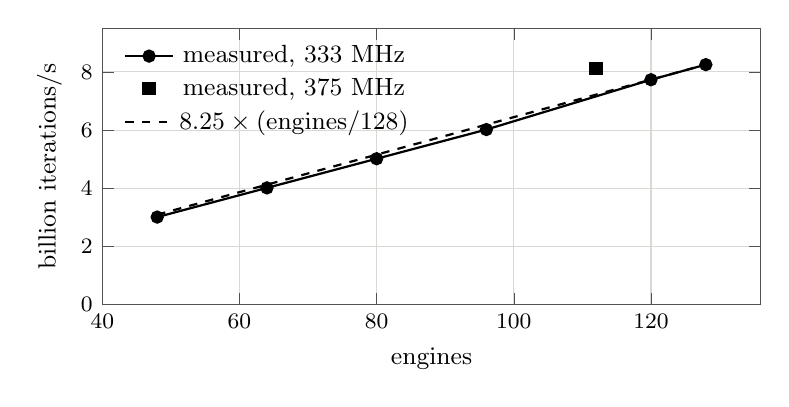
\begin{tikzpicture}
\begin{axis}[
  width=0.82\textwidth,
  height=0.42\textwidth,
  xlabel={engines},
  ylabel={billion iterations/s},
  xmin=40, xmax=136,
  ymin=0, ymax=9.5,
  grid=major,
  legend style={at={(0.02,0.98)},anchor=north west,font=\small},
]
\addplot[mark=*,thick] coordinates {
  (48,3.0107) (64,4.0137) (80,5.0158) (96,6.018) (120,7.73) (128,8.249)
};
\addlegendentry{measured, $333$~MHz}
\addplot[mark=square*,only marks,thick] coordinates { (112,8.123) };
\addlegendentry{measured, $375$~MHz}
\addplot[dashed,domain=48:128,thick] {0.06445*x};
\addlegendentry{$8.25\times(\mathrm{engines}/128)$}
\end{axis}
\end{tikzpicture}
\caption{ECC2K-130 FPGA engine on AWS F2. The 128-engine image at
  $333$~MHz is $8.25$~billion iterations/s; the pre-board estimate was
  $5$--$12$ billion iterations/s with a central $8$. The measurement landed on the
  central estimate; it is a device measurement, not the estimate
  restated.}
\label{fig:fpga}
\end{figure}

Per engine the current revision is $6{,}790$--$6{,}940$ LUTs, $9{,}371$
FFs, 12 RAMB36, 4 URAM and 66 DSPs; the 96-engine image used $62\%$ of
the LUTs and $81\%$ of the block RAM, and block RAM, not logic, is
what bounds the engine count on this part~\evcite{\evref{hdl}}.

\subsection{FPGA vs.\ GPU}
\label{sec:fpga-vs-gpu}

At the prices observed on 2026-09-11, an F2 instance at $\$1.980$
on demand or $\$0.709$ spot against an RTX~PRO~6000 at $\$4.14$ and
$\$1.31$ per GPU-hour, the expected $2^{60.9}$ iterations cost about $72{,}400$
F2-hours at the measured $8.25$~billion iterations/s, roughly $\$51$k spot, against
$42{,}400$ GPU-hours and $\$56$k spot at the campaign's $14.11$~billion iterations/s
collection rate.\footnote{Derived here from the measured rate and the
prices recorded in \evref{fpgaest}; the note's own
table priced the hypothetical $8$~billion iterations/s image at $\$53$k spot.} So
the two platforms are level on cost per solve, within the noise of spot
pricing, and the FPGA is about $2$--$5\times$ better per watt on the
note's estimated power envelopes ($75$--$150$~W against a $600$~W
board). FPGA workers follow the same client contract as the GPUs and
write the same records, so a collision between an FPGA trail and a GPU
trail is merged like any other.

\section{Campaign}
\label{sec:campaign}

At the campaign's collection rate, $2^{60.9}$ iterations is about
five years on a single GPU. The campaign is therefore not a single
solve but a collection effort: a corpus of distinguished points, each
re-walkable from its seed, grown on whatever hardware is cheapest at
the time and merged as it arrives. This section covers its
configuration, its calibration, its storage protocol and where it
stands now.

\subsection{Configuration}

The configuration is one file in the repository; the copy in the
storage bucket is what workers read~\evcite{\evref{ops}; \evref{ops}}. Walk: $\sigma$ (Section~\ref{sec:walk-sigma}). \texttt{dpWeight}: 32,
uniform campaign-wide, and a campaign run refuses any other. Batch 16,
256-thread blocks, two resident blocks per SM, $385{,}024$ workers
$=6{,}160{,}384$ logical walks per GPU, $1{,}024$ steps per launch,
checkpoint and upload every 600~s, restart every 48~h. The iteration guard \texttt{maxIters} in the repository file is
$2^{32}$, twelve trail lengths at weight 32; it was $2^{30}$, three
trail lengths, which a model on the measured rates says cut $4.9\%$ of
walks and discarded $15.6\%$ of the fleet's steps until an audit found
it. Whether the bucket copy was raised before the fleet stopped is not
recorded~\evcite{\evref{audit}}. The fields
that define the corpus (workers, batch, geometry, curve, cutoff, walk
and the state-layout knobs) freeze once any slot exists;
\texttt{WITNESS=0} is pinned. The preset is the audited RTX~PRO~6000 build at CUDA~13.3.1 and
\texttt{sm\_120}~\evcite{\evref{ops}}. A checkpoint is about
370~MB (six million walks at 60 bytes).

\subsection{Distinguished-point cutoff}
\label{sec:campaign-interval}

The planning numbers follow from the cutoff~\evcite{\evref{ops}, ``The numbers that decide the plan''}.
At weight 34 the expected corpus is $2^{35.6}$ records, about $1.7$~TB,
one per $2^{25.27}$ iterations; at weight 32 one report per $2^{28.41}$
iterations, $2^{3.14}=8.8\times$ rarer, so about $2^{32.5}$ records and
$0.19$~TB at the expected work, about 40 points/s, $3.4$~M points/day
and $0.11$~GB/day from a GPU collecting at $14.11$~billion iterations/s. The price of a
rarer point is the work left in flight when a collision lands: $43$
GPU-hours per GPU at weight 32 ($6.16$~M walks times $2^{28.41}$
steps), $13\%$ of the expected work at 128 GPUs and more than the
whole expected work at $1{,}024$, against $4.9$ GPU-hours per GPU at
weight 34. The campaign's fleet size never approached the range where
that trade reverses.

We measured the interval twice, and the first measurement was
wrong. A fleet-wide ratio of $7.93\cdot10^{15}$ checkpointed
iterations to $31.6$~M uploaded points on 2026-09-15 had been quoted
as $2^{27.9}$ iterations per point. Neither counter was clean: the
checkpoint sum multiplied every slot's per-walk base by the Blackwell
grid constant, inflating the auto-sized Ada slots by the ratio of the
grids (about $26\times$ on an L4-sized grid), and the point total mixed in two retired slots that had walked at weight 34. The
replacement reads from each live worker the client's own two
counters, iterations this run on the grid the client built itself and
points reported over the same interval, frozen at 2026-09-17 18:47~UTC
across 132 workers (Table~\ref{tab:cutoff})~\evcite{\evref{dpint}}.
The result, $2^{28.41}=3.56\cdot10^8$, is the same on every hardware
family to $0.04$ in the exponent, and sits $2^{0.60}$ below the naive
binomial $P(\HW\le32)=2^{-29.01}$, as Bailey et al.'s $2^{25.27}$ sits
$2^{0.57}$ below the binomial at weight 34. We classify the
correction as accounting: the walk did not change, only the number
did, and we retire the earlier figure rather than averaging it in.

\begin{table}[t]
\centering
\small
\caption{Iterations per distinguished point at cutoff 32, frozen
  2026-09-17 18:47~UTC. Per-worker spread $0.04$ in the exponent. The
  last column is the median self-reported rate of the family's
  workers on the same day.}
\label{tab:cutoff}
\begin{tabular}{@{}lrrrrr@{}}
\toprule
family & workers & iterations & points & it/point & median billion it/s \\
\midrule
RTX PRO 6000 (\texttt{g7e}) & 38 & $5.606\cdot10^{15}$ & $15{,}724{,}672$ & $2^{28.41}$ & 14.66 \\
L40S (\texttt{g6e}) & 34 & $2.723\cdot10^{15}$ & $7{,}643{,}600$ & $2^{28.41}$ & 7.47 \\
RTX PRO 4500 (\texttt{g7}) & 48 & $3.081\cdot10^{15}$ & $8{,}640{,}973$ & $2^{28.41}$ & 4.87 \\
CPU & 12 & $2.804\cdot10^{14}$ & $785{,}410$ & $2^{28.41}$ & 2.29 \\
\midrule
all & 132 & $1.169\cdot10^{16}$ & $32{,}794{,}655$ & $\mathbf{2^{28.41}}$ & $\approx1{,}068$ total \\
\bottomrule
\end{tabular}
\end{table}

\subsection{Cost}
\label{sec:campaign-goal28}

The total cost depends on the work, not on the size of the fleet: at the
2026-09-11 spot price of $\$1.31$ per RTX~PRO~6000 hour the expected
$42{,}400$ GPU-hours are about $\$56$k whether 8 GPUs take 221 days or
512 take $3.4$; on demand the figure is $\$142$k--$\$175$k~\evcite{\evref{ops}}.
What fleet size changes is the calendar, and the in-flight loss
described above. The campaign ran mixed families because iterations per
dollar, not iterations per card, is the objective: on 2026-09-18 the best-value quote was an L4 in \texttt{eu-north-1}
at $56\cdot10^{12}$ iterations per dollar against $38\cdot10^{12}$ for the
RTX~PRO~6000 and $28\cdot10^{12}$ for the RTX~PRO~4500, and at that
quote a full reference walk costs about
$\$38$k~\evcite{\evref{quotes}}. The per-SKU rates
behind those ratios are measured, not list: L40S $8.84$~billion iterations/s with
\texttt{clmad}, L4 $2.49$, T4 $0.53$ without it~\evcite{\evref{ada}; \evref{t4}}.

The RTX~PRO~4500 is the most instructive case. Its measured $5.107$~billion iterations/s on
the shipping walk is exactly what the 6000's rate predicts from SM
count and clock ($14.64\times82/188\times1.95/2.44=5.10$), and at that rate the 6000 wins per dollar by $1.2$--$1.3\times$; the
break-even against the 6000's shipping rate is $6.2$--$6.6$~billion iterations/s in the
two cheapest regions and $8.8$ in the third, figures the note says
must be redone with both cards on their best
builds~\evcite{\evref{pro4500}}. That
is why a $12$~billion iterations/s goal was set for the card and why the $x$-only
bridge map of Section~\ref{sec:walk-bridge} was pursued there rather
than on the 6000: a power-capped die rewards fewer instructions per
step more than a pipe-bound one does. The separate goal of $28$~billion iterations/s on
one 6000 was priced below the pipe (Section~\ref{sec:floor}) and its
grid and occupancy screens, run on an RTX~PRO~4500 because no 6000
could be allocated, found nothing faster than the shipping
configuration~\evcite{\evref{goal28}}.

A power survey closes the loop: on the 6000 the $20$~billion iterations/s build drew
$583$~W for $34.4$~M updates per joule and a fused-pass variant
$544$~W for $37.0$~M/J in the same session, $1.072\times$ per joule in
five paired repetitions against a $1.03$ target; per joule, not per
second, is the figure that transfers to a $165$~W card, and the model,
calibrated on the 4500's $5.107$ and $5.552$~billion iterations/s receipts (ratio error
$+2.6\%$), predicts $7.2$--$7.4$~billion iterations/s for the fused build
there~\evcite{\evref{power}}. That prediction still
needs a measurement; the bridge map got there first.

\subsection{Storage and certification}
\label{sec:campaign-storage}

A record is 32 bytes: a little-endian 64-bit seed and the canonical
normal-basis $x$ of the endpoint, three 64-bit words; no scalar
coefficients are stored, they are rebuilt by replay. The seed is \texttt{run id (16) $\|$ walk index (32) $\|$ restart
counter (16)} with run id $=$ slot $+1$; a splitmix64 finaliser
expands it to the 128-bit $c$ of the start point. Two contributors who
pick different run ids never start the same walk (independently
seeded walks can still meet, which is the point), and a permanent seed
registry does compare-and-set across providers (Modal GPU runs are ids
8000--8999, CPU sidecars 9000--9999); a race test with eight claimants
acquired exactly one~\evcite{\evref{cert}; \evref{cert}; \evref{audit}, ``Seeds''; \evref{ops}}.

Uploads are ordered so that no pointer ever names data that is not
there: payloads before their commit manifests, both before checkpoint
publication. Strict manifests bind curve, cutoff, guard, seed and key
semantics, worker geometry, source hash, worker binary hash and
replay binary hash, and every immutable payload carries its SHA-256.
Slot ownership is one S3 object per slot claimed with a conditional
put on the ETag, a 60~s heartbeat and a 180~s lease; checkpoints are
content-addressed and the owner-checked heartbeat publishes the
pointer, so a stale worker can leave orphaned blobs but cannot commit.
The note is explicit that this is integrity against failure, not
authentication against an actor able to rewrite both data and
manifests~\evcite{\evref{cert}; \evref{ops}, ``Slots''}.

Merging buckets records by a hash of the key limbs (the first layout
used the key's low bits) into $4{,}096$ files, sorts, drops exact duplicates (the client store, the database primary
key and the merge are three layers; $9.95$~M re-reports had been
dropped by 2026-09-25) and reports equal keys with different seeds.
Such a pair goes into a two-record file and to the CPU client, which
re-walks both trails, aligns Frobenius and negation, and verifies
$[k]P=Q$; a $\mathrm{GF}(2^{41})$ pair with known seeds that recovers
$k=369250562913$ is the local acceptance fixture. An exhaustive check of $76{,}904{,}684$ step multisets confirms that
no multiset of at most 32 $\sigma$-walk steps closes an orbit, so no
short fruitless cycle exists; a trail crossing itself at random is
estimated at about $2^{-65}$ per trail, about $10^{-10}$ over the
campaign, and the iteration guard releases such a
walk~\evcite{\evref{cert}; \evref{audit}; \evref{ops}}.

The public dashboard publishes aggregates only: not point keys,
coefficients, seeds or database locations~\evcite{\evref{status}; \evref{status}}.

\subsection{Status}
\label{sec:campaign-state}

The campaign was created on 2026-09-11. Its fleet on 2026-09-17 was about 133 workers (the 132 with enough
points to calibrate are in Table~\ref{tab:cutoff}), producing about
$2{,}600$ points/s by the ingest's count; the ingest path was re-engineered that week from one object
at a time ($2{,}450$ records/s, below production) to a threaded loader
measured at $137{,}753$ rows/s, and a five-and-a-half-hour blind spot during a key layout change was
recovered in 23 minutes ($4{,}321$ objects,
$63{,}351{,}803$ rows, zero failed), taking the store from $67.6$~M to
$124.3$~M points~\evcite{\evref{ops}}. On 2026-09-18 the spot market reclaimed every worker and the cloud
account was placed on an account-verification (risk) hold that has
blocked new instance launches since; collection continued at a small
scale on another provider. Its first four GPU runs reused the run ids
of the first four slots by mistake and re-walked them ($813$k of one
run's $912$k records byte-identical to the slot they replayed, all
dropped as re-reports, and an inadvertent end-to-end replay check);
later runs use the reserved ids
8000--8999~\evcite{\evref{hold}; \evref{client}, ``Collecting for the campaign from Modal''}.

Table~\ref{tab:state} gives two snapshots: the audited one of
2026-09-25, while a small fleet was still walking, and the published
feed of 2026-10-10, by which time the last point had landed
(2026-10-07) and no slot was walking; the sustained peak and the
mean trail length in the caption are from the
audit~\evcite{\evref{audit}; \evref{feed}; \evref{audit}}.
Having no collision yet is exactly what we should expect: $2^{56.68}$ iterations is $5.4\%$
of $2^{60.9}$, and the probability of no collision after a fraction
$c$ of the expected work is about $\exp(-\pi c^2/4)$, here $0.998$.
Collection is paused, not finished: every slot's checkpoint and the
corpus are intact, and a worker that resumes a slot continues its
walks from the checkpoint.

\begin{table}[t]
\centering
\small
\caption{Campaign state at the audited snapshot of 2026-09-25
  05:05~UTC and at the published feed of 2026-10-10 15:42~UTC. The pooled iterations-per-point ratio is below $2^{28.41}$, partly
  because the corpus still holds weight-34 records from the first two
  slots; the mean length of walks that ended by 2026-09-25 is
  $2^{28.34}$. Sustained production peaked at about $842{,}000$ points
  per hour on 2026-09-23, about $83$~billion iterations/s.}
\label{tab:state}
\begin{tabular}{@{}lrr@{}}
\toprule
 & 2026-09-25 & 2026-10-10 \\
\midrule
distinguished points stored & $367{,}123{,}410$ & $485{,}528{,}850$ \\
iterations (checkpointed) & $2^{56.38}$ & $2^{56.68}$ \\
share of expected work & $4.4\%$ & $5.4\%$ \\
collisions & 0 & 0 \\
duplicate re-reports dropped & $9{,}953{,}494$ & $14{,}153{,}833$ \\
slots / walking / off-weight & 195 / 2 / 7 & 227 / 0 / 7 \\
points in the last 24~h & $741{,}048$ & 0 \\
walk rate over the last hour & $3.65$~billion iterations/s & 0 \\
last point stored & --- & 2026-10-07 14:41 \\
\bottomrule
\end{tabular}
\end{table}

\section{Upper bounds}
\label{sec:bounds}

Everything in this paper is engineering against a fixed exponent, so the
natural question is how much engineering is left. We answer it per
platform with ceilings derived from measured pipe rates: each assumes the
named unit runs at its full measured rate and that every other cost is
zero. They are upper bounds, not forecasts. Figure~\ref{fig:bounds}
draws them against today's measurements.

% x: billion iterations per second, 0.37 cm per unit.
\begin{figure}[t]
\centering
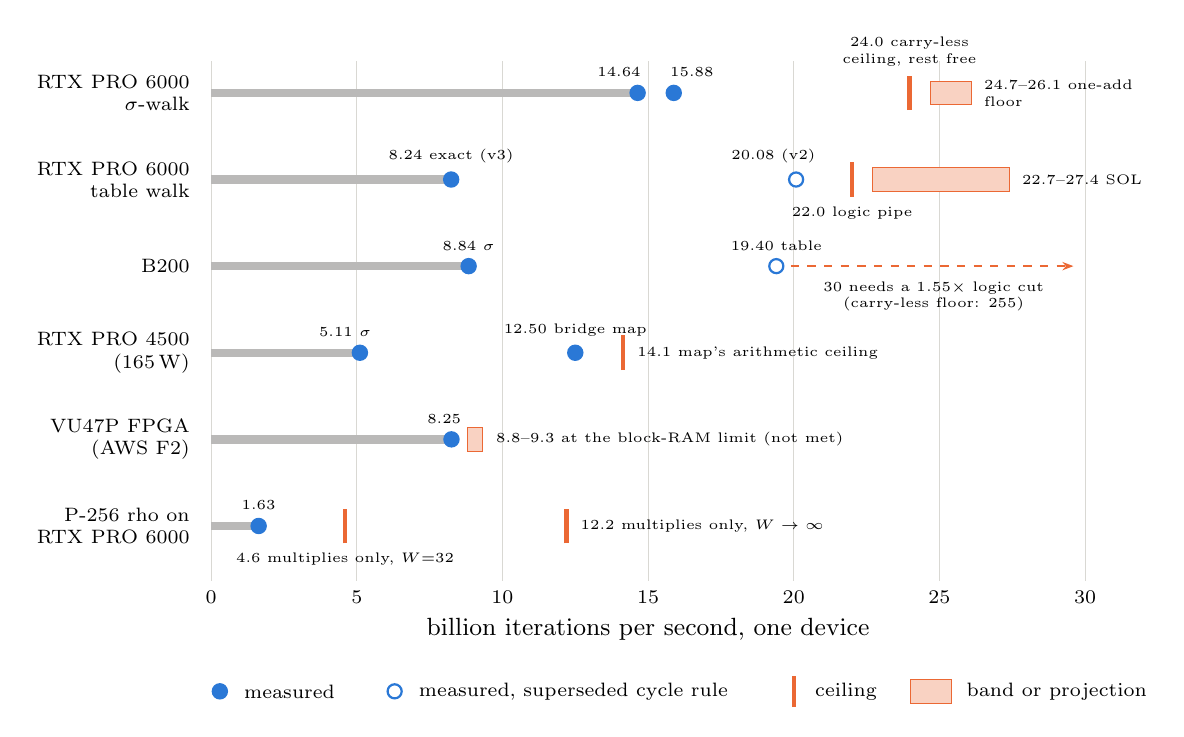
\begin{tikzpicture}[font=\scriptsize,x=0.37cm,y=1cm,
  meas/.style={circle,fill=cA,inner sep=2.1pt},
  old/.style={circle,draw=cA,fill=white,thick,inner sep=1.8pt},
  ceil/.style={draw=cB,line width=1.6pt},
  band/.style={fill=cB!30,draw=cB},
  lab/.style={anchor=east,align=right,font=\scriptsize}]
% grid
\foreach \v in {0,5,10,15,20,25,30}{
  \draw[gridc] (\v,0.4) -- (\v,-6.2);
  \node[below,font=\scriptsize] at (\v,-6.2) {\v};
}
\node[below=10pt,font=\small] at (15,-6.2) {billion iterations per second, one device};
% Row 1: RTX PRO 6000 sigma
\node[lab] at (-0.4,0) {RTX PRO 6000\\$\sigma$-walk};
\draw[inkS!40,line width=3pt] (0,0) -- (14.64,0);
\node[meas] at (14.64,0) {}; \node[meas] at (15.88,0) {};
\node[above,font=\tiny] at (14.0,0.08) {14.64};
\node[above,font=\tiny] at (16.5,0.08) {15.88};
\draw[ceil] (23.97,-0.22) -- (23.97,0.22); \node[above,font=\tiny,align=center] at (23.97,0.22) {24.0 carry-less\\ceiling, rest free};
\fill[band] (24.7,-0.15) rectangle (26.1,0.15);
\node[right,font=\tiny,align=left] at (26.2,0) {24.7--26.1 one-add\\floor};
% Row 2: RTX PRO 6000 table
\node[lab] at (-0.4,-1.1) {RTX PRO 6000\\table walk};
\draw[inkS!40,line width=3pt] (0,-1.1) -- (8.24,-1.1);
\node[meas] at (8.24,-1.1) {}; \node[above,font=\tiny] at (8.24,-1.02) {8.24 exact (v3)};
\node[old] at (20.08,-1.1) {}; \node[above,font=\tiny] at (19.3,-1.02) {20.08 (v2)};
\draw[ceil] (22.0,-1.32) -- (22.0,-0.88); \node[below,font=\tiny] at (22.0,-1.32) {22.0 logic pipe};
\fill[band] (22.7,-1.25) rectangle (27.4,-0.95); \node[right,font=\tiny] at (27.5,-1.1) {22.7--27.4 SOL};
% Row 3: B200
\node[lab] at (-0.4,-2.2) {B200};
\draw[inkS!40,line width=3pt] (0,-2.2) -- (8.84,-2.2);
\node[meas] at (8.84,-2.2) {}; \node[above,font=\tiny] at (8.84,-2.12) {8.84 $\sigma$};
\node[old] at (19.40,-2.2) {}; \node[above,font=\tiny] at (19.40,-2.12) {19.40 table};
\draw[-{Stealth[length=4pt]},dashed,cB,thick] (19.9,-2.2) -- (29.6,-2.2);
\node[below,font=\tiny,align=center] at (24.8,-2.27) {30 needs a $1.55\times$ logic cut\\(carry-less floor: 255)};
% Row 4: RTX PRO 4500
\node[lab] at (-0.4,-3.3) {RTX PRO 4500\\(165\,W)};
\draw[inkS!40,line width=3pt] (0,-3.3) -- (5.107,-3.3);
\node[meas] at (5.107,-3.3) {}; \node[above,font=\tiny] at (4.6,-3.22) {5.11 $\sigma$};
\node[meas] at (12.50,-3.3) {}; \node[above,font=\tiny] at (12.5,-3.22) {12.50 bridge map};
\draw[ceil] (14.14,-3.52) -- (14.14,-3.08); \node[right,font=\tiny] at (14.3,-3.3) {14.1 map's arithmetic ceiling};
% Row 5: FPGA
\node[lab] at (-0.4,-4.4) {VU47P FPGA\\(AWS F2)};
\draw[inkS!40,line width=3pt] (0,-4.4) -- (8.25,-4.4);
\node[meas] at (8.25,-4.4) {}; \node[above,font=\tiny] at (8.0,-4.32) {8.25};
\fill[band] (8.8,-4.55) rectangle (9.3,-4.25); \node[right,font=\tiny] at (9.45,-4.4) {8.8--9.3 at the block-RAM limit (not met)};
% Row 6: NIST
\node[lab] at (-0.4,-5.5) {P-256 rho on\\RTX PRO 6000};
\draw[inkS!40,line width=3pt] (0,-5.5) -- (1.632,-5.5);
\node[meas] at (1.632,-5.5) {}; \node[above,font=\tiny] at (1.632,-5.42) {1.63};
\draw[ceil] (4.6,-5.72) -- (4.6,-5.28); \node[below,font=\tiny] at (4.6,-5.72) {4.6 multiplies only, $W{=}32$};
\draw[ceil] (12.2,-5.72) -- (12.2,-5.28); \node[right,font=\tiny] at (12.35,-5.5) {12.2 multiplies only, $W\to\infty$};
% key
\begin{scope}[shift={(0,-7.6)}]
\node[meas] at (0.3,0) {}; \node[anchor=west] at (0.8,0) {measured};
\node[old] at (6.3,0) {}; \node[anchor=west] at (6.8,0) {measured, superseded cycle rule};
\draw[ceil] (20.0,-0.2) -- (20.0,0.2); \node[anchor=west] at (20.4,0) {ceiling};
\fill[band] (24.0,-0.15) rectangle (25.4,0.15); \node[anchor=west] at (25.6,0) {band or projection};
\end{scope}
\end{tikzpicture}
\caption{How far each platform can go, against what it does today.
  Ceilings are derived from measured pipe rates with every other cost
  set to zero, so they are upper bounds, not targets: the RTX~PRO~6000's
  are its carry-less and logic pipes for any walk with one affine
  addition per step (Section~\ref{sec:floor}); the NIST bounds count only
  field multiplications at the measured multiply rate
  (Section~\ref{sec:bounds-nist}). None of these moves the $2^{60.9}$
  iteration count.}
\label{fig:bounds}
\end{figure}


\subsection{RTX~PRO~6000}
\label{sec:bounds-6000}

The ceiling for any walk that performs one affine addition per step is
set by two pipes (Section~\ref{sec:floor}). On the carry-less unit,
$28.9$ \texttt{CLMAD} per update at $1.65$ lanes per SM-clock caps the card
at $24.7$--$26.1$ billion iterations per second with everything else
free; on the logic pipe, the arithmetic alone already needs more slots
than $28$ allows~\evcite{\evref{iterfn}, §1}. The roofline of the table
walk's build puts its own speed of light between $22.7$ and $27.4$,
depending on how fast \texttt{CLMAD} sustains in that kernel's
instruction mix, and the logic pipe binds first, at
$22.0$~\evcite{\evref{roofline}, §2 and §4}. For the $\sigma$-walk with its
current carry-less arithmetic ($38.125$ \texttt{CLMAD} per update at two
lanes), the same calculation gives about $24.0$ with every other cost
free~\evcite{\evref{sparse}}.

So the realistic headroom on one card is about $1.5\times$: from $15.88$
for the best $\sigma$-walk to the low or middle twenties, and only by
cutting integer work. Thirty is out of reach for any one-addition walk
on this card; it would need integer work cut from about $1{,}320$ to $968$
lane-instructions per update with the carry-less unit fully busy, which
the note calls a two-card number~\evcite{\evref{roofline}, §5}. Two cards at
today's rates already exceed it.

\subsection{Other GPUs}
\label{sec:bounds-other}

On the B200 the carry-less unit is so fast that its floor, $255$ billion
iterations per second, is irrelevant; the logic pipe is the only
ceiling. Thirty would need at most $618$ logic slots per update against
$955$ after the sweep, a $1.55\times$ cut, and the candidate offloads
(reduction, basis conversions and branch selection as carry-less
operations) add up to roughly that, though none has been
built~\evcite{\evref{twochains}, §6.2 and §6.5; \evref{autosweep}, §3.4}.
The H100 would need at most $521$ slots for the same
rate~\evcite{\evref{twochains}, §6.5}. On the power-capped RTX~PRO~4500,
the bridge map's own arithmetic ceiling is $14.1$, measured with the
rest of the map stripped out, so $15$ is not available on that map
either~\evcite{\evref{bridge}}.

\subsection{FPGA}
\label{sec:bounds-fpga}

The F2 engine scales linearly with engine count and is bounded by block
RAM, not logic. At $5.16$ clocks per step the projection is $8.8$ billion
iterations per second at 136 engines and $9.3$ at 144 engines or at 128
engines and 375~MHz; the 144-engine build failed placement and the
375~MHz builds missed timing, so neither is met~\evcite{\evref{hdl}}.
About $13\%$ above today's $8.25$ is all this part offers without a new
design.

\subsection{NIST curves}
\label{sec:bounds-nist}

The prime-field walk has more room, because it is further from any
ceiling. A step costs about $6 + 320/W$ field multiplications: three for
the affine addition, three for Montgomery's trick, and a share of a
Fermat inversion with a four-bit window (about 256 squarings and 64
multiplications; our count). At the measured $73.4$ billion dependent
multiplications per second on P-256, that caps the walk at about $4.6$
billion iterations per second at $W=32$ and $12.2$ as $W$ grows without
limit. The walk runs at $1.632$, the cost of about 45 multiplications per
step against 16 counted, so roughly two thirds of each step is still
outside the multiplier: selection, distinguished-point checks, loads and
the serial latency of each thread's inversion. These bounds are ours,
derived from the measured multiply rate, and that rate is itself a
single dependent chain, so a throughput-bound multiplier would raise
them~\evcite{\evref{nistres}}.

\subsection{Cost per solve}
\label{sec:bounds-cost}

Cost per solve scales inversely with the rate. At the campaign's
collection rate of $14.11$ billion iterations per second the expected
$2^{60.9}$ iterations are $42{,}400$ RTX~PRO~6000 hours, about \$56k at the
2026-09-11 spot price~\evcite{\evref{ops}}. If the $\sigma$-walk reached
$24$ the same work would be about $24{,}900$ GPU-hours and \$33k, and at
$26$, about $23{,}000$ GPU-hours and \$30k (our scaling of the measured
figures). Even the ceiling leaves the solve a five-figure rental
problem. No engineering in this paper or in the bounds above changes
the $2^{60.9}$; only an algorithmic advance would. Section~\ref{sec:solvetime} turns these rates
into calendar time for fleets of each kind of device.

\section{Time to solve}
\label{sec:solvetime}

The rates in this paper translate directly into calendar time and
money, and this section does that translation for every device we
measured. Nothing here is a new measurement: each estimate divides the
expected work by a rate recorded earlier in the paper and states what
else it assumes. The question for ECC2K-130 is no longer whether a solve
is feasible but how many cards, for how long, at what price. For the
NIST curves, the same arithmetic gives an answer that no plausible
amount of hardware changes.

\subsection{Model}
\label{sec:solvetime-model}

Three quantities set the time to a collision.

\paragraph{Expected work.} The $\sigma$-walk needs $2^{60.9}\approx2.15\cdot10^{18}$
iterations in expectation (Section~\ref{sec:walk-constant}). One
device running at $R$ billion iterations per second therefore needs
$2.15\cdot10^{18}/R$ nanoseconds, or $68.2/R$ years
(Table~\ref{tab:history-compare}), and a fleet of $N$ such devices
needs $1/N$ of that.

\paragraph{Variance.} Rho's running time is random. The probability
of no collision after a fraction $c$ of the expected work is about
$\exp(-\pi c^2/4)$ (Section~\ref{sec:campaign-state}). Half of all
solves finish by $c=0.94$, nine in ten by $c=1.71$ and 99 in 100 by
$c=2.42$ (our arithmetic). So a plan that must finish with $90\%$
probability should budget $1.7$ times the expected work.

\paragraph{Detection delay.} A collision is only seen when the
second of the two merged trails reaches a distinguished point. At
cutoff 32 that is on average another $2^{28.41}$ steps of one walk
(Section~\ref{sec:campaign-interval}). Each walk advances at $R$
divided by the number of walks on the card. With $6.16$ million walks
on an RTX~PRO~6000, the delay is about $42$ hours at $14.64$ and $38$
hours at $15.88$, whatever the fleet size (our arithmetic; the campaign
note gives $43$ GPU-hours per GPU at $14.11$~\evcite{\evref{ops}}).
Every card keeps walking during the delay, so a large fleet pays for it
in GPU-hours as well as calendar time. At 1{,}000 cards it adds about
as much work as the solve itself. Cutoff 34 cuts the delay to about
$4.4$ hours at $15.88$, at the cost of an $8.8\times$ larger corpus
(about $1.7$~TB instead of $0.19$~TB).

A fleet of $N$ devices at $R$ therefore expects a collision after
\[
  T(N) \approx \frac{2^{60.9}}{N\,R} + D,
\]
where $D$ is the detection delay. The first term is multiplied by $0.94$
for the median and by $1.71$ for a $90\%$ plan.

\paragraph{Existing corpus.} The campaign has already walked $2^{56.68}$
iterations without a collision (Table~\ref{tab:state}). A new fleet
that runs the same $\sigma$-walk at cutoff 32 and merges with that
corpus inherits the credit. Given no collision so far, the expected
remaining work is $0.949$ of the total (our arithmetic). That is a
saving of $5\%$; it changes the plan, not the scale.

\subsection{By device and fleet size}
\label{sec:solvetime-table}

Table~\ref{tab:solvetime} applies the first term of the model to every
rate in this paper. The $\sigma$-walk rows are the survey and paired
rates of Table~\ref{tab:survey}. Points from these rows can merge with
the campaign corpus. The other rows use other walks or other platforms.

\begin{table}[t]
\centering
\footnotesize
\setlength{\tabcolsep}{4pt}
\caption{Expected time to walk $2^{60.9}$ iterations of ECC2K-130 at
  each recorded rate, our arithmetic. ``Years, one'': device-years on a
  single device. ``Days, 100'' and ``Days, 1{,}000'': calendar days for
  a fleet of that size, excluding the detection delay $D$ (about
  $1.6$--$1.7$ days on the RTX~PRO~6000 at cutoff 32). The median is
  $0.94\times$ these figures and the $90\%$ point $1.71\times$. ``Cost'':
  the expected work at the Modal list price implied by
  Table~\ref{tab:survey}'s iterations per dollar (2026-09-19). Spot
  prices are much lower (text). Table-walk rates are absent because no
  table-walk build has a measured cost per solve
  (Section~\ref{sec:sigma-vs-table}).}
\label{tab:solvetime}
\begin{tabular}{@{}llrrrrr@{}}
\toprule
device & build & billion it/s & years, one & days, 100 & days, 1{,}000 & cost \\
\midrule
\multicolumn{7}{@{}l}{\emph{$\sigma$-walk (merges with the campaign corpus)}} \\
RTX PRO 6000 & campaign preset & 14.64 & 4.66 & 17.0 & 1.70 & \$124k \\
RTX PRO 6000 & nibble-table $\sigma$ & 15.88 & 4.29 & 15.7 & 1.57 & \$114k \\
L40S & survey & 8.70 & 7.84 & 28.6 & 2.86 & \$134k \\
B200 & survey & 8.84 & 7.71 & 28.2 & 2.82 & \$423k \\
B300 & survey & 7.58 & 9.00 & 32.9 & 3.29 & \$560k \\
H200 & survey & 7.63 & 8.93 & 32.6 & 3.26 & \$356k \\
H100 & survey & 7.54 & 9.04 & 33.0 & 3.30 & \$313k \\
A100-80GB & survey & 4.63 & 14.7 & 53.8 & 5.38 & \$323k \\
L4 & survey & 2.56 & 26.6 & 97.2 & 9.72 & \$186k \\
A10 & survey & 2.42 & 28.1 & 102.8 & 10.3 & \$272k \\
T4 & no \texttt{clmad} & 0.541 & 126 & 460 & 46.0 & \$652k \\
\addlinespace
\multicolumn{7}{@{}l}{\emph{other walks and platforms}} \\
RTX PRO 4500 & $x$-only bridge map & 12.50 & 5.46 & 19.9 & 1.99 & --- \\
RTX PRO 4500 & $\sigma$-walk & 5.11 & 13.3 & 48.8 & 4.88 & --- \\
VU47P (AWS F2) & 128 engines & 8.25 & 8.26 & 30.2 & 3.02 & --- \\
Xeon, one core & AVX-512 bitsliced & 0.0126 & 5{,}410 & --- & --- & --- \\
\addlinespace
\multicolumn{7}{@{}l}{\emph{bound and history}} \\
RTX PRO 6000 & ceiling (Section~\ref{sec:bounds-6000}) & 24--26 & 2.6--2.8 & 9.6--10.4 & 0.96--1.04 & --- \\
GTX 295 card & 2010 kernel & 0.064 & 1{,}065 & 3{,}891 & 389 & --- \\
\bottomrule
\end{tabular}
\end{table}

% Expected days = 2^60.9 / (N R) / 86400 = 24896 / (N R) for R in billion it/s.
% Plotted parametrically in log10(N) so the curves sample evenly on the log axis.
\begin{figure}[t]
\centering
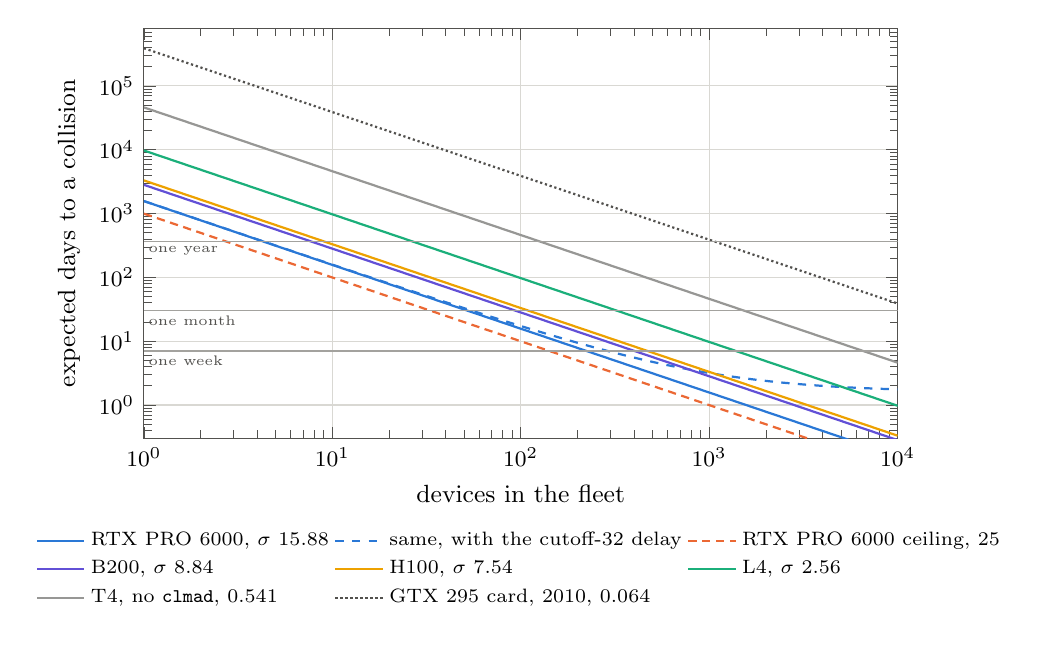
\begin{tikzpicture}
\begin{loglogaxis}[
  width=0.92\textwidth, height=0.56\textwidth,
  xmin=1, xmax=10000, ymin=0.3, ymax=8e5,
  xlabel={devices in the fleet},
  ylabel={expected days to a collision},
  xmajorgrids, ymajorgrids,
  legend style={at={(0.5,-0.2)},anchor=north,font=\scriptsize},
  legend columns=3, legend cell align=left,
  every axis plot/.append style={thick},
]
\addplot[cA,domain=0:4,samples=2] ({10^x},{24896/(15.884*10^x)});
\addlegendentry{RTX PRO 6000, $\sigma$ 15.88}
\addplot[cA,dashed,domain=0:4,samples=60] ({10^x},{24896/(15.884*10^x)+1.6});
\addlegendentry{same, with the cutoff-32 delay}
\addplot[cB,densely dashed,domain=0:4,samples=2] ({10^x},{24896/(25*10^x)});
\addlegendentry{RTX PRO 6000 ceiling, 25}
\addplot[cE,domain=0:4,samples=2] ({10^x},{24896/(8.840*10^x)});
\addlegendentry{B200, $\sigma$ 8.84}
\addplot[cD,domain=0:4,samples=2] ({10^x},{24896/(7.540*10^x)});
\addlegendentry{H100, $\sigma$ 7.54}
\addplot[cC,domain=0:4,samples=2] ({10^x},{24896/(2.561*10^x)});
\addlegendentry{L4, $\sigma$ 2.56}
\addplot[inkS!60,domain=0:4,samples=2] ({10^x},{24896/(0.541*10^x)});
\addlegendentry{T4, no \texttt{clmad}, 0.541}
\addplot[inkS,densely dotted,domain=0:4,samples=2] ({10^x},{24896/(0.064*10^x)});
\addlegendentry{GTX 295 card, 2010, 0.064}
% calendar references
\draw[gridc!60!inkS,line width=0.4pt] (axis cs:1,7) -- (axis cs:10000,7);
\node[anchor=north west,font=\tiny,text=inkS,inner sep=1.5pt] at (axis cs:1,7) {one week};
\draw[gridc!60!inkS,line width=0.4pt] (axis cs:1,30) -- (axis cs:10000,30);
\node[anchor=north west,font=\tiny,text=inkS,inner sep=1.5pt] at (axis cs:1,30) {one month};
\draw[gridc!60!inkS,line width=0.4pt] (axis cs:1,365) -- (axis cs:10000,365);
\node[anchor=north west,font=\tiny,text=inkS,inner sep=1.5pt] at (axis cs:1,365) {one year};
\end{loglogaxis}
\end{tikzpicture}
\caption{Expected calendar time to walk $2^{60.9}$ iterations of
  ECC2K-130 against fleet size, at measured one-device rates in billions
  of iterations per second (Table~\ref{tab:solvetime}), with the 2010
  GTX~295 for comparison. Solid lines count walking time only. The
  dashed line adds the RTX~PRO~6000's detection delay at cutoff 32
  (about $1.6$ days), which sets a floor that more cards cannot lower.
  The median solve is $0.94\times$ the plotted time and the $90\%$
  point $1.71\times$.}
\label{fig:solvetime}
\end{figure}


On the best card, a solve is about four device-years. A fleet of five
RTX~PRO~6000s finishes in about a year. With 56 the expected time is a
month, including the detection delay. With 290 it is a week. A thousand
cards bring the expected time down to about $3.2$ days, $1.6$ of
walking and $1.6$ of waiting for the last trail to reach a
distinguished point. Nine times in ten, a thousand cards finish within
$4.3$ days. Beyond a few hundred cards the delay dominates, which is
where Figure~\ref{fig:solvetime}'s dashed line bends away from the
solid one. A larger fleet buys little calendar time unless it also
lowers the cutoff.

The new GPUs moved this by more than two orders of magnitude. With the
2010 kernel on a GTX~295, a one-year solve needed about 1{,}066 cards
and a one-week solve more than $55{,}000$. Today the same one-year and
one-week targets need five cards and 290. If the RTX~PRO~6000 reached
its ceiling, the solve would be about $2.7$ device-years. Even the
campaign's own peak, about $83$~billion iterations/s from a mixed spot
fleet (Table~\ref{tab:state}), would finish the remaining expected
work in about $285$ days.

\paragraph{Cost.} The cost of the work does not depend on the size of
the fleet. At Modal list prices the cheapest per solve are the
RTX~PRO~6000 and the L40S, about \$114k--\$134k. The data-centre
Blackwell and Hopper parts cost two and a half to five times as much
for the same work, because this integer-bound walk does not use what
they are priced for (Section~\ref{sec:survey}). Spot capacity is
cheaper again. At the 2026-09-11 spot price of \$1.31 per RTX~PRO~6000
hour the expected work is about \$56k at the campaign's collection rate
of $14.11$. An AWS F2 at its spot price comes to about \$51k
(Section~\ref{sec:fpga-vs-gpu}). The best quote seen, an L4 in
\texttt{eu-north-1} on 2026-09-18, priced a full walk at about
\$38k~\evcite{\evref{ops}; \evref{quotes}}. Those spot figures hold only
while spot capacity lasts. The spot market reclaimed the campaign's
whole fleet on 2026-09-18 (Section~\ref{sec:campaign-state}), and a
solve on spot capacity has to plan for that.

\paragraph{Assumptions.} Every rate in
Table~\ref{tab:solvetime} is sustained for the whole solve. The survey
rows are single unpaired runs, and the campaign's own fleet measured
its RTX~PRO~6000 workers at a median of $14.66$
(Table~\ref{tab:cutoff}), so the survey rates are close to what a fleet
sees but are not guaranteed. The bridge map on the RTX~PRO~4500 walks a
different function, so its points do not merge with the
$\sigma$-walk corpus. Its frozen study measured $1.007\times$ the work
of the map it replaced (Section~\ref{sec:walk-bridge}). The FPGA row is
one card of an \texttt{f2.6xlarge}. The CPU row is one core and assumes
the per-core rate holds across a server. The costs exclude storage,
egress and the merge.

\subsection{NIST curves}
\label{sec:solvetime-nist}

The same model applies to the NIST walk of Section~\ref{sec:nist}, and
it shows why that section's rates say nothing about the security of
those curves. With the negation map, the expected work for a group of
prime order $n$ is about $\sqrt{\pi n/4}$ iterations. For P-256 that is
$2^{127.8}\approx3.0\cdot10^{38}$ iterations, and for P-384
$2^{191.8}\approx5.6\cdot10^{57}$ (our arithmetic from the standard group
orders; any walk constant above one only adds to it).
\begin{itemize}[nosep]
\item \textbf{P-256.} At the best measured $1.632$~billion
  iterations/s on one RTX~PRO~6000, the expected time is $1.9\cdot10^{29}$
  seconds, about $5.9\cdot10^{21}$ card-years. A billion cards would
  need $5.9\cdot10^{12}$ years, more than 400 times the age of the
  universe.
  At the multiplies-only bound of $12.2$ (Section~\ref{sec:bounds-nist})
  it is still $7.8\cdot10^{20}$ card-years.
\item \textbf{P-384.} At $0.548$ the expected time is $1.0\cdot10^{49}$
  seconds, about $3.2\cdot10^{41}$ card-years.
\end{itemize}
The engineering of Section~\ref{sec:nist} multiplied the P-256 rate by
$1.52$ and the P-384 rate by $2.61$, and divided these times by the
same factors. P-256 needs about $2^{67}$ times the work of ECC2K-130, so
a speedup of any engineering size leaves it where it was. The levers
that bring ECC2K-130 within a fleet's reach shorten a P-256 attack by a
factor that disappears against the exponent.

\section{Open problems}
\label{sec:open}

This section collects what we would try next, and what would settle
each question. Some items carry an estimate from the note that
proposed them; we quote those as estimates, not results. None of them
moves the exponent. What they could move is the constant, and on
Blackwell the constant is still being found.

\subsection{Table walk}
\label{sec:open-table}

The biggest open question is whether a correct table walk can be made
faster than the $\sigma$-walk again. The $20.08$~billion iterations/s
build ran cycle rule v2, whose exits from a fruitless cycle depended on
how a trail had entered it. That was found in review and fixed by rule
v3, which picks one exit for each detected cycle regardless of
history (Section~\ref{sec:walk-cycles}). The exact v3 kernel runs at
$8.24$~billion iterations/s in its latest screen ($5.10$ in its first
paired panel), against $15.88$ for the best
$\sigma$-walk~\evcite{\evref{client}, ``The earlier 20.078 B/s table result''; \evref{v3}; \evref{redesign}}.
Almost all of that gap is the cost of probing for cycles inside the
critical path, and several ideas attack it:
\begin{itemize}[leftmargin=1.2em,itemsep=0.2em]
\item \emph{Deferred cycle detection (a rule v4).} Detect cycles after
  the fact rather than on every hinted step. The note estimates this
  recovers ``most of the gap, 15--19'' billion iterations/s, but it is
  a new rule identity, so the reference model, the corpus header and
  the replay and walk-constant tools all have to move with
  it~\evcite{\evref{probelat}, §3.1}.
\item \emph{A cheaper probe step} in the polynomial basis (estimated at
  $30$--$45\%$ of the probe's critical path, implemented and passing the
  host probe, not yet re-measured on a device), and \emph{early
  termination} of the probe through the formal $\ZZ[\tau]$ sum
  (estimated $-35\%$ probe work)~\evcite{\evref{probelat}, §3.2--3.3}.
\item \emph{Moving the probe off the critical path} onto a concurrent
  resolver, at an estimated $4.5\%$ of ALU work with its latency
  hidden~\evcite{\evref{probelat}, §3.4--3.5}.
\item \emph{The paired cost-per-solve run.} Even a fast exact table
  walk only pays if its cost per solve beats the $\sigma$-walk's. The
  v2 projection was $0.81$--$0.86\times$, which held only while the table
  walk kept at least $0.932$--$0.943$ of the $\sigma$-walk's rate, and
  only for the first $15$--$22\%$ of a campaign. The paired run that would
  test it has never been executed; its job script is all that
  exists~\evcite{\evref{walkconst}, §11.1 and §11.5}.
\end{itemize}

\subsection{$\sigma$-walk}
\label{sec:open-sigma}

The $\sigma$-walk is at $15.88$~billion iterations/s on one RTX~PRO~6000,
and the repository's one-card goal of $26$ is unmet. The roofline says
where the slack is. The polynomial reduction is the largest single
item, $29\%$ of the integer work, and the path to $30$~billion
iterations/s needs integer work cut from about $1{,}320$ to $968$
lane-instructions per update with the carry-less unit fully busy,
which the note calls a two-card number~\evcite{\evref{roofline}, §2 and §5}.
Open items:
\begin{itemize}[leftmargin=1.2em,itemsep=0.2em]
\item A shared-memory square table for the $\sigma$-walk compiles and
  fits on \texttt{sm\_120}; its device occupancy and paired rate are
  pending~\evcite{\evref{sigmasq}}.
\item Toom-3 over $\FF_2$ is not implemented. A Karatsuba-family search
  found nothing below $8{,}859$ bitsliced instructions, but the packed
  kernel's product has never been tried in Toom form~\evcite{\evref{client}, ``What is not done''}.
\item On the RTX~PRO~4500, the bridge map's collection rate at cutoff 34
  is unmeasured, and a pre-registered rare-phase skip has not been
  run~\evcite{\evref{bridge}}.
\end{itemize}

\subsection{Blackwell pipes}
\label{sec:open-pipes}

Three questions about the hardware itself would sharpen every estimate
above.
\begin{itemize}[leftmargin=1.2em,itemsep=0.2em]
\item \emph{Is the integer-multiply pipe separate from the logic pipe?}
  If it is, moving shifts onto \texttt{IMAD.SHL} is the next integer
  lever; if the two share a datapath, the kernel is already at $96\%$.
  A small probe settles it: a $1{:}1$ \texttt{LOP3}/\texttt{IMAD} mix
  running at $1.5\times$ or more says separate, under $1.2\times$ says
  shared. It has not been run~\evcite{\evref{roofline}, §4.1 and §7}.
\item \emph{What does \texttt{CLMAD} sustain in the walk's own
  instruction mix?} The carry-less speed of light for the table walk
  lies between $22.7$ and $27.4$~billion iterations/s depending on
  whether paired \texttt{CLMAD}s beside a 40-\texttt{LOP3} chain reach
  $1.90$ lanes per SM-clock or stop at $1.70$. A screened three-limb
  Karatsuba arm implies at least $1.654$; a verified run would pin
  it~\evcite{\evref{roofline}, §3, §4.2 and §7}.
\item \emph{Hardware counters.} Nsight Compute last read counters on
  the $17.4$ build; it failed on the rented RTX~PRO~4500 and cannot read
  counters inside Modal containers, so the utilisation of the $20.08$
  build and later comes from instruction counts
  (Section~\ref{sec:profiling}). A host with working counters would
  replace those estimates with measurements~\evcite{\evref{goal28}, ``Nsight findings''}.
\end{itemize}

\subsection{Data-centre GPUs}
\label{sec:open-gpus}

Kernel tuning does not transfer between dies. The B200's three winning
knobs (fused pass, batch 32, three-limb Karatsuba) are among the RTX
PRO~6000's largest losses, so every new part needs its own
sweep~\evcite{\evref{autosweep}, §4}. On the B200 the logic pipe
binds hard, and $30$~billion iterations/s would need at most $618$ ALU
slots per update against $955$ after the sweep. The candidate offloads
all move work onto the carry-less unit: the reduction as products
against the modulus ($-290$ ALU, $+19$ \texttt{CLMAD}), the basis
conversions and Frobenius networks as carry-less linear maps (about
$300$ slots), and the branch selection as polynomial evaluation (about
$175$). None has been built~\evcite{\evref{twochains}, §6.2 and §6.5; \evref{autosweep}, §3.4}.
The B300 is an open case: NVIDIA cut its FP64 rate to $1/64$ of
FP32~\cite{aubrey2025blackwellultra}, and if \texttt{CLMAD} runs on the
FP64 pipe there as it does elsewhere, the B300 would price carry-less
work like the workstation die rather than like the B200. Its
$\sigma$-walk is already slower per SM than the B200's ($51.2$ against
$59.7$ million iterations per second), but the probe of
Table~\ref{tab:clmad-dies} has not been run on it. The H100 has been probed but never run the kernel. On the power-capped
RTX~PRO~4500, the fused build is predicted at $7.2$--$7.4$~billion
iterations/s on the shipping walk from an energy model calibrated on one
pair, and a single run would confirm or break the
model~\evcite{\evref{power}, §4--5}. Multi-GPU instances are not
implemented: one process drives one device.

\subsection{NIST curves}
\label{sec:open-nist}

The prime-field walk has had two rounds of tuning, so its open
questions are nearer the surface:
\begin{itemize}[leftmargin=1.2em,itemsep=0.2em]
\item \emph{$W=64$.} Both curves now sit at the 255-register ceiling at
  $W=32$, so $W=64$ will probably spill and lose; one cell would
  confirm it.
\item \emph{Separating the round-2 gain} between the larger batch and the
  by-reference inversion, with a $W=32$ cell built without the new
  inversion.
\item \emph{A Solinas-field walk.} The field benchmark favours Solinas
  for the P-384 multiplication; the walk has never been built on it.
\item \emph{Independent chains per thread, reseeding off the critical
  path, and a second walk per table read}, each named as a next rung
  in the results file but not yet priced~\evcite{\evref{nistres}; \evref{nist}, ``Measurement rule''}.
\item \emph{A larger jump table.} The walk uses $2^8$ entries, so a
  fruitless two-cycle starts about once every 512 steps. The secp256k1
  notes estimate that going to $2^{11}$ cuts the escape work eightfold;
  the same argument applies here, untested~\evcite{\evref{eccopt}, §4.1--4.3}.
\item \emph{Repeated, interleaved pairs} for the best cell against its
  control, which would turn the single-run ratios of
  Table~\ref{tab:nist-ladder} into intervals.
\end{itemize}

\subsection{CPUs}
\label{sec:open-cpu}

The CPU side has had the least attention and has the clearest
untested levers.
\begin{itemize}[leftmargin=1.2em,itemsep=0.2em]
\item \emph{A packed $\sigma$-walk on x86 with VPCLMULQDQ.} The packed
  client's carry-less path has no measurement on x86 and walks only the
  table walk. AVX-512's \texttt{vpclmulqdq} does four
  $64\times64$ products per instruction, and AMD's Zen~5 and Intel's
  current server cores run AVX-512 at full width; nobody has measured
  either~\evcite{\evref{cpupacked}}.
\item \emph{Arm's newer vector extensions.} SVE2's \texttt{PMULLB}/\texttt{PMULLT}
  and its three-input \texttt{EOR3}/\texttt{BCAX} would serve both the
  packed and the bitsliced client on Neoverse V-class cores; none of
  the code uses SVE today.
\item \emph{Prime fields with real carry chains.} A four-limb Montgomery
  multiply with \texttt{MULX}/\texttt{ADX}, or 52-bit limbs on AVX-512
  IFMA, would replace the big-integer reference solver; this is the CPU
  version of the GPU's PTX carry-chain step and has not been tried for
  rho~\evcite{\evref{nistcpu}}.
\item \emph{GFNI after a layout change.} GFNI wins on small-field basis
  changes but was priced as a loss for ECC2K-130's bitsliced conversions
  because it acts on bytes within a register; a byte-oriented layout
  could change that verdict~\evcite{\evref{gfni}}.
\end{itemize}

\subsection{Methodology}
\label{sec:open-method}

Two lessons from this work are worth keeping as rules. Static
instruction counts are not throughput: two candidates predicted from
their static counts at $0.887$ and $0.976$ measured $0.986$ and $0.905$ on
the device~\evcite{\evref{nativecand}; \evref{g7native}}.
And a rate is not a cost per solve: every engineering gain in this
paper is a same-walk scheduling result until a paired run on the walk
constant says otherwise. Tensor cores, finally, remain a negative
result for this walk: they need one operand shared across eight or
sixteen lanes, and no product in the walk has
one~\evcite{\evref{twochains}, §1}.

\section{Related work}
\label{sec:related}

\paragraph{The 2009 attempt.} Bailey et al.~\cite{bailey2009} fixed
the iteration function this campaign walks, $R\mapsto\sigma^j(R)+R$
with $j$ from the weight of $x$, the weight-34 distinguished-point
rule, and the $2^{60.9}$ budget, and reported per-platform rates on
Core~2 (533 cycles per iteration with 128-bit vectors), Cell, GPUs,
FPGAs~\cite{fan2010fpga} and ASIC estimates; their SHARCS
paper~\cite{bailey2009sharcs} priced the whole Certicom ECC2 list.
Bos, Kleinjung, Niederhagen and Schwabe's Cell
implementation~\cite{bos2010cell} is the bitsliced lineage this
client's CPU and first GPU backends belong to. The GPU line ends with
Bernstein et al.'s GTX~295 kernel~\cite{bernstein2010gpu}, which
reached $1{,}164$ cycles per iteration per multiprocessor and about $64$
million iterations per second per card; Niederhagen's
thesis~\cite{niederhagen2012thesis} collects the final Cell and GPU
figures. We found no later published ECC2K-130 rate for any GPU
generation between Fermi and Blackwell, which is part of why
Section~\ref{sec:history} compares directly against 2010. The type-II
optimal-polynomial-basis multiplication of Bernstein and
Lange~\cite{bernsteinlange2010onb} is used verbatim; the conversion
networks generated here match their hand-designed chains to within a
few instructions (Section~\ref{sec:arith-bitsliced}). Bernstein's bit
operation counts for binary multiplication~\cite{bernstein2009batch}
are the reference the three-input-logic finding is measured against.
Bernstein et al.'s later FPGA designs~\cite{bernstein2016fpga}, which
set the current size record for a completed binary-curve computation
by solving a $2^{117.35}$-order instance on sect113r2 and were
extrapolated to a 127-bit field, are the calibration for the pre-board
estimate of Section~\ref{sec:fpga}, which the measurement then met. Between those two, Wenger and Wolfger solved
a 113-bit Koblitz-curve logarithm on a Virtex-6 cluster at one
iteration per clock~\cite{wenger2014sac} and then a 113-bit binary
curve on Kintex-7 parts~\cite{wenger2016jce}.
Harley's group solved ECC2K-95 in 1998 and ECC2K-108 in April 2000,
the latter with about $1{,}300$ volunteers' machines over four
months~\cite{harley1998,harley2000}; those two are the only Koblitz
challenges completed, and their walks are the ancestors of the one in
Section~\ref{sec:walk-sigma}.

\paragraph{Rho on automorphism classes.} The $\sqrt{2m}$ saving from
Frobenius and negation on Koblitz curves is due to Wiener and
Zuccherato~\cite{wienerzuccherato1998} and Gallant, Lambert and
Vanstone~\cite{glv2000}, generalised by Duursma, Gaudry and
Morain~\cite{duursma1999}. Teske's $r$-adding walks~\cite{teske2001}
and the Bernstein--Lange--Schwabe treatment of fruitless cycles under
the negation map~\cite{bls2011} are the background to
Section~\ref{sec:walk-table}; the cycle classes measured there are the
$\tau$-relation analogue, and the measured walk constants of
Table~\ref{tab:walkconst} are, to our knowledge, the first reported
for this branch distribution on this family. The distinguished-point
method is van Oorschot and Wiener's~\cite{vanoorschot1999}. The 112-bit
prime-field record of Bos et al.~\cite{bos2012ps3} is the nearest
completed computation in scale.

\paragraph{Measurement discipline.} The companion
paper~\cite{ecdlppaper} states the boundary-unit-table-class rule and
applies it across rho, baby-step giant-step and kangaroo; this paper is, in effect, its ECC2K-130 chapter at
full length.

\paragraph{Prime-field rho on GPUs.} Bos et al.'s 112-bit record on
PlayStation~3 consoles~\cite{bos2012ps3} is the nearest completed
prime-field computation in scale. Our NIST walk (Section~\ref{sec:nist})
reuses the standard ingredients, an $r$-adding walk~\cite{teske2001},
the negation map with fruitless-cycle handling~\cite{bls2011} and
Montgomery's simultaneous inversion~\cite{montgomery1987}; what it adds
is a measured account of which GPU optimisations from the binary
campaign carry over to it.

\section{Conclusion}
\label{sec:conclusion}

We summarise the state of Pollard rho on current NVIDIA hardware as
measured in this work.

\paragraph{Per-card throughput.} In 2010 the
best GTX~295 kernel ran ECC2K-130 at $0.064$ billion iterations per
second. On one RTX~PRO~6000 Blackwell the same walk runs at $14.64$ in
the audited campaign build and $15.88$ in the best later build, and the
whole $2^{60.9}$ budget is about five GPU-years. Roughly a sixth of that
factor is a bigger, faster chip; the rest is arithmetic. Sixteen paired
steps took the client from a $0.85$ bitsliced control to $14.64$, and
three representation changes did most of the work: Frobenius
permutation networks, the native carry-less product, and the smaller
batch that the native product made possible.

\paragraph{Time to solution.} At $15.88$ billion
iterations per second, five RTX~PRO~6000s expect to find the collision
in about a year, 56 in a month, 290 in a week, and a thousand in about
three days, half of them spent waiting for the last trail to reach a
distinguished point at cutoff 32. The work costs about \$114k at list
price and \$38k--\$56k on the spot quotes we saw, whatever the fleet
size. The same rates leave P-256 about $6\cdot10^{21}$ card-years away
(Section~\ref{sec:solvetime}).

\paragraph{Carry-less multiplication across dies.}
PTX~9.3 gives every part from \texttt{sm\_80} onward a carry-less
multiply, but not at the same rate. On the RTX~PRO~6000 it issues at
about $1.7$ lanes per SM-clock, the cost of $38$ logic instructions; on
the B200 and H100 it is ten to eighteen times faster. The workstation
part still wins on this walk, per card, per SM and per dollar, because
the walk is bound by integer logic and the RTX~PRO~6000 has the most
SMs at the highest clock for the money. On the data-centre parts the
logic pipe binds instead, the right kernel moves work onto the
carry-less unit, and kernel tuning does not travel between them. For
any walk with one affine addition per step, $28$ billion iterations per
second on one RTX~PRO~6000 is out of reach on both pipes.

\paragraph{Choice of iteration function.} The table walk
does the arithmetic of a step more cheaply, and reached $20.08$ under
cycle rule v2. But v2's exits from fruitless cycles depended on how a
trail arrived, and the exact v3 rule that fixes this runs at $8.24$
today, about half the $\sigma$-walk's rate. Closing that gap, with a deferred or off-critical-path cycle
check, is the largest open optimisation in this paper, and even then a
table walk must win on cost per solve, which nobody has measured.

\paragraph{Transfer to prime fields.} On NIST P-256 and P-384 on the same card, explicit carry
chains, a wider shared inversion and the same refusal of register-cap
trades gave $1.52\times$ and $2.61\times$, to $1.632$ and $0.548$ billion
iterations per second. The batch width, a modest knob on the binary
walk, was the biggest lever on the prime one, because a Fermat
inversion costs some forty times as many multiplications as a
normal-basis one. A P-256 step remains about nine times as expensive
as an ECC2K-130 step on the same card, which is the carry-less unit's
advantage in one number.

\paragraph{Remaining headroom.} None of the speedup
came from changing the algorithm: every step kept Bailey et al.'s walk
and its distinguished points bit for bit, and the gains split into
representation and arithmetic ($6.3\times$), batch and geometry
($1.5\times$), memory layout ($1.3\times$) and the new instruction
($1.2\times$). The same pipe measurements bound what is left. Any walk with
one affine addition per step tops out at about $24$--$26$ billion
iterations per second on one RTX~PRO~6000, so the best $\sigma$-walk has
roughly $1.5\times$ to go, all of it in integer work; a B200 would need a
$1.55\times$ cut in logic instructions to reach $30$; the F2 FPGA stops near
$9.3$. On CPUs the instruction sets matter as much as on GPUs: three-input
logic and wider words give $2.4$--$3\times$ to the bitsliced client.

\paragraph{Asymptotic cost and the campaign.} The campaign's walk needs $2^{60.91}$--$2^{60.92}$ iterations,
which agrees with the 2009 estimate. The campaign stored $486$ million
points and $2^{56.68}$ iterations, $5.4\%$ of the expected work, with no
collision, every record re-walkable from its seed; its fleet was
reclaimed on 2026-09-18 and collection is paused. Whether the remaining
$94.6\%$ is walked is a question of money, not mathematics, and at five
GPU-years it is a much smaller question than it was in 2009.

\appendix
\section{Reproduction}
\label{app:repro}

The companion repository~\cite{rhoblackwell}, \url{https://github.com/aburan28/rho-blackwell}, carries the
ECC2K-130 client (CUDA and CPU), the NIST P-256/P-384 rho kernel, the
paper source, the benchmark data behind every figure, the evidence
records of Appendix~\ref{app:evidence}, and a Dockerfile.

\paragraph{Status.} The CPU client, its validation suite, a
planted-logarithm solve and every mode of the image's entry point have
been run from the repository's copy of the source; the Docker image
itself has not yet been built, and its GPU modes have not been run. The
commands below describe the intended workflow.

\paragraph{Docker.} The image compiles the client with CUDA~13.3 for
Ampere, Ada, Hopper and both Blackwell families, with the audited
RTX~PRO~6000 preset (the $\sigma$-walk, batch 16, 256-thread blocks,
native \texttt{clmad}, compact tiled state and shared Frobenius masks),
and runs the client's validation suite during the build. By default a
container walks ECC2K-130 with the campaign's parameters (cutoff 32, a
$2^{32}$ iteration guard, checkpoints every ten minutes) on the GPU if one
is visible and on the CPU otherwise, writing 32-byte distinguished-point
records and a resumable checkpoint to its data volume:
{\small\begin{verbatim}
docker build -t rho-blackwell -f docker/Dockerfile .
docker run --gpus all -v rho-data:/data rho-blackwell   # walk ECC2K-130
docker run --gpus all rho-blackwell bench                # throughput only
docker run rho-blackwell test                             # validation suite
docker run rho-blackwell planted                          # small planted logs
docker run --gpus all rho-blackwell ecc2k95               # ECC2K-95, answer known
docker run --gpus all rho-blackwell nist                  # P-256/P-384 rho bench
\end{verbatim}}
A container without \texttt{RUN\_ID} picks a random run identifier from
a range the campaign never used (20000--65535), keeps it with its data
and warns that it did so. Two containers with the same identifier walk
the same trails, and with random choices that happens with probability
about $0.1\%$ for 10 containers, $10\%$ for 100 and $63\%$ for 300, so any
run of more than one container must assign each a distinct
\texttt{RUN\_ID}. A collision is
found by merging the corpora of all containers that walked with the
same cutoff; a single container is unlikely to find one alone.

\paragraph{Building without Docker.} The client needs a C++17 compiler
and, for the GPU build, CUDA~13.3 or newer (the native carry-less product
requires PTX~9.3). Its make targets build the CPU client, the GPU client
with any preset of this paper, and the test suites; the repository's
README lists the targets for each measured build, including the fused
and nibble-table $\sigma$-walks and the B200 and RTX~PRO~4500 presets.

\paragraph{Checking a number.} Every measured number cites an evidence
record [E$n$]. The repository's \texttt{evidence/} directory holds each
record under its number, with the notes, data or source that report the
measurement, so a reader can check a number without the development
history; \texttt{evidence/map.json} names the original file of each.

\section{Evidence records}
\label{app:evidence}

Every measured number in this paper cites one of the records below as
[E$n$], optionally with a section of that record. Each record is a
measurement report, dataset, protocol or source file kept in a public
repository named after its title. The companion repository being
prepared for this paper (Appendix~\ref{app:repro}) will hold a copy of
every record under its number.

{\small
\begin{description}[leftmargin=2.6em,labelwidth=2.2em,itemsep=0.1em,font=\normalfont]
\item[\evlabel{client}{E1}] ECC2K-130 client reference: field, walk, validation and throughput. \emph{design and measurement notes}; crypto.
\item[\evlabel{cmodel}{E2}] Independent C golden model of $\FF_{2^{131}}$ and the curve. \emph{source and tests}; cryptanalysis.
\item[\evlabel{codegen}{E3}] Field model and code generator for $\FF_{2^{131}}$. \emph{source}; crypto.
\item[\evlabel{hdl}{E4}] FPGA engine: VHDL design, reference model and test vectors. \emph{design and source}; crypto.
\item[\evlabel{ecc2k95}{E5}] ECC2K-95 GPU kernel and Koblitz pair table. \emph{design notes and source}; crypto.
\item[\evlabel{walkconst}{E6}] Walk constants and fruitless-cycle analysis on toy Koblitz curves. \emph{measurement report}; crypto.
\item[\evlabel{witness}{E7}] Witness counters and their cost. \emph{measurement report}; crypto.
\item[\evlabel{ops}{E8}] Campaign operations, configuration and planning numbers. \emph{operations notes}; crypto.
\item[\evlabel{sigmafused}{E9}] Fused single-pass $\sigma$-walk. \emph{paired benchmark}; crypto.
\item[\evlabel{iterfn}{E10}] Iteration functions compared: $\sigma$-walk, table walk and their cost model. \emph{measurement report}; crypto.
\item[\evlabel{bridge}{E11}] $x$-only doubling-and-bridge map on the RTX PRO 4500. \emph{paired benchmark}; crypto.
\item[\evlabel{maxiters}{E12}] Iteration-guard study. \emph{analysis}; crypto.
\item[\evlabel{v3}{E13}] Table-walk cycle escape, rule v3. \emph{design and measurement notes}; crypto.
\item[\evlabel{packedsrc}{E14}] Packed $\FF_{2^{131}}$ arithmetic for CUDA. \emph{source}; crypto.
\item[\evlabel{ceiling}{E15}] Instruction-issue rates and the throughput ceiling. \emph{measurement report}; crypto.
\item[\evlabel{packed}{E16}] Ledger: packed normal-basis backend and its audit. \emph{paired benchmark}; crypto.
\item[\evlabel{frobnet}{E17}] Ledger: Frobenius permutation networks. \emph{paired benchmark}; crypto.
\item[\evlabel{clmad}{E18}] Ledger: native carry-less multiplication (\texttt{clmad}). \emph{paired benchmark}; crypto.
\item[\evlabel{roofline}{E19}] Roofline of the table-walk build on the RTX PRO 6000. \emph{measurement report}; crypto.
\item[\evlabel{refsrc}{E20}] Host reference implementation of the step. \emph{source}; crypto.
\item[\evlabel{ecc2k95clmad}{E21}] ECC2K-95 kernel: \texttt{clmad} port. \emph{measurement report}; crypto.
\item[\evlabel{ada}{E22}] Ada L4 and L40S with and without \texttt{clmad}. \emph{measurement report}; crypto.
\item[\evlabel{t4}{E23}] Turing T4 without \texttt{clmad}. \emph{measurement report}; crypto.
\item[\evlabel{twochains}{E24}] Two-chain kernel and \texttt{CLMAD} rates on three dies. \emph{measurement report}; crypto.
\item[\evlabel{topclmad}{E25}] Declined: top-bit correction on \texttt{CLMAD}. \emph{paired benchmark}; crypto.
\item[\evlabel{autosweep}{E26}] Automatic single-knob sweep on the B200 and RTX PRO 6000. \emph{measurement report}; crypto.
\item[\evlabel{nativecand}{E27}] Native-instruction candidates and the acceptance rule. \emph{protocol}; crypto.
\item[\evlabel{sigmatable}{E28}] $\sigma$ step through shared-memory nibble tables. \emph{paired benchmark}; crypto.
\item[\evlabel{singleprod}{E29}] Ledger: single polynomial product. \emph{paired benchmark}; crypto.
\item[\evlabel{dencache}{E30}] Ledger: denominator cache. \emph{paired benchmark}; crypto.
\item[\evlabel{polychain}{E31}] Ledger: polynomial-basis batch chain. \emph{paired benchmark}; crypto.
\item[\evlabel{pairedprod}{E32}] Ledger: paired products. \emph{paired benchmark}; crypto.
\item[\evlabel{polystate}{E33}] Ledger: polynomial-basis state. \emph{paired benchmark}; crypto.
\item[\evlabel{directred}{E34}] Ledger: direct reduction. \emph{paired benchmark}; crypto.
\item[\evlabel{genprod}{E35}] Ledger: generated straight-line product. \emph{paired benchmark}; crypto.
\item[\evlabel{tiles}{E36}] Ledger: 256-worker tiles. \emph{paired benchmark}; crypto.
\item[\evlabel{batch}{E37}] Ledger: batch 16 with 385{,}024 workers. \emph{paired benchmark}; crypto.
\item[\evlabel{wprefix}{E38}] Ledger: weighted prefixes and paired Frobenius. \emph{paired benchmark}; crypto.
\item[\evlabel{compact}{E39}] Ledger: compact 17-byte state and batch screens. \emph{paired benchmark}; crypto.
\item[\evlabel{sharedsigma}{E40}] Ledger: shared-memory mask table. \emph{paired benchmark}; crypto.
\item[\evlabel{tablecmp}{E41}] Table walk against $\sigma$-walk: paired comparison data. \emph{dataset}; crypto.
\item[\evlabel{oneblock}{E42}] One-block table-walk geometry (the 20.08 build). \emph{paired benchmark}; crypto.
\item[\evlabel{survey}{E43}] Eleven-GPU survey on Modal. \emph{measurement report}; crypto.
\item[\evlabel{tuning}{E44}] Declined: stream-Karatsuba compile option. \emph{benchmark}; crypto.
\item[\evlabel{addcombine}{E45}] Declined: integer add in the carry-less product. \emph{paired benchmark}; crypto.
\item[\evlabel{lambda}{E46}] Declined: $\lambda$-projective coordinates, priced. \emph{analysis}; crypto.
\item[\evlabel{hostsched}{E47}] AVX-512 host scheduling pass. \emph{measurement report}; crypto.
\item[\evlabel{dpint}{E48}] Distinguished-point interval calibration at cutoff 32. \emph{measurement report and raw counters}; crypto.
\item[\evlabel{nistres}{E49}] NIST P-256/P-384 rho on the RTX PRO 6000: device results, rounds 1 and 2 (round 2: the $W=32$ and register-cap cells, merged in pull request 1778). \emph{measurement report}; crypto.
\item[\evlabel{nist}{E50}] NIST P-256/P-384 GPU library: field, walk and tests. \emph{design notes and source}; crypto.
\item[\evlabel{nistproto}{E51}] Pre-registered NIST GPU arithmetic protocol. \emph{protocol}; crypto.
\item[\evlabel{nistcpu}{E52}] Fifteen-curve NIST ECDLP solver and audit. \emph{design and measurement notes}; crypto.
\item[\evlabel{ecc}{E53}] secp256k1 GPU library: field, walk, folds and baby-step giant-step. \emph{design notes and source}; crypto.
\item[\evlabel{kangaroo}{E54}] GPU kangaroo interval solver. \emph{design and measurement notes}; crypto.
\item[\evlabel{nistattempt}{E55}] First NIST GPU attempt (infrastructure non-result). \emph{record}; crypto.
\item[\evlabel{prho64}{E56}] 64-bit prime-field GPU rho. \emph{design and measurement notes}; cryptanalysis.
\item[\evlabel{eccopt}{E57}] secp256k1 GPU arithmetic: Blackwell optimisation notes. \emph{analysis}; crypto.
\item[\evlabel{gpueff}{E58}] GPU efficiency scorer and the packed-walk profile. \emph{tool and profile}; cryptanalysis.
\item[\evlabel{fpgaest}{E59}] FPGA pre-board estimate. \emph{analysis}; crypto.
\item[\evlabel{f2}{E60}] FPGA engine on AWS F2: builds and measurements. \emph{measurement report}; crypto.
\item[\evlabel{audit}{E61}] Campaign audit and live snapshot, 2026-09-25. \emph{audit report and dataset}; crypto.
\item[\evlabel{quotes}{E62}] Fleet price quotes, 2026-09-18. \emph{operations record}; crypto.
\item[\evlabel{pro4500}{E63}] RTX PRO 4500: rates and per-dollar break-even. \emph{measurement report}; crypto.
\item[\evlabel{goal28}{E64}] The 28-billion goal: grid and occupancy screens. \emph{measurement report}; crypto.
\item[\evlabel{power}{E65}] Power-bound model and updates per joule. \emph{measurement report}; crypto.
\item[\evlabel{cert}{E66}] Storage, seeds and certification protocol. \emph{protocol}; crypto.
\item[\evlabel{status}{E67}] Public campaign dashboard. \emph{documentation}; crypto.
\item[\evlabel{hold}{E68}] Cloud account hold, 2026-09-18. \emph{operations record}; crypto.
\item[\evlabel{feed}{E69}] Published campaign feed, 2026-10-10. \emph{dataset}; crypto.
\item[\evlabel{probelat}{E70}] Cycle-probe latency and the routes to a faster exact rule. \emph{analysis}; crypto.
\item[\evlabel{sigmasq}{E71}] $\sigma$-walk shared-memory square table: compile and resource gate. \emph{gate record}; crypto.
\item[\evlabel{g7native}{E72}] Native-instruction candidates on the RTX PRO 4500. \emph{paired benchmark}; crypto.
\item[\evlabel{sparse}{E73}] Sparse-basis and compound $\sigma$ maps: modelled ceilings. \emph{analysis}; crypto.
\item[\evlabel{cpupacked}{E74}] Packed CPU client on PMULL/PCLMULQDQ. \emph{design and measurement notes}; cryptanalysis.
\item[\evlabel{gfni}{E75}] GFNI for basis changes: measured on small fields, priced for ECC2K-130. \emph{measurement report and analysis}; crypto.
\item[\evlabel{smallclmul}{E76}] Carry-less reduction in small binary fields (PCLMULQDQ). \emph{measurement report}; crypto.
\item[\evlabel{redesign}{E77}] Iteration-function redesign screens, 2026-10-12: the tuned v3 table walk and a two-card $\sigma$-walk aggregate. \emph{screen reports}; crypto.
\item[\evlabel{tp29}{E78}] Throughput rounds toward 29 billion iterations/s on the RTX PRO 6000, with Nsight Compute counters. \emph{design and measurement notes}; crypto.
\item[\evlabel{probes}{E79}] Instruction-rate probes and static SASS cost tools. \emph{microbenchmarks and tools}; crypto.
\item[\evlabel{rhoopt}{E80}] Strong-rho canonicalisation on small Koblitz curves: instruction-count result (unmerged branch). \emph{measurement report}; crypto.
\end{description}
}


\bibliographystyle{plainnat}
\bibliography{rho-blackwell}

\end{document}
